\documentclass{book}
\usepackage[a4paper,top=2.5cm,bottom=2.5cm,left=2.5cm,right=2.5cm]{geometry}
\usepackage{makeidx}
\usepackage{natbib}
\usepackage{graphicx}
\usepackage{multicol}
\usepackage{float}
\usepackage{listings}
\usepackage{color}
\usepackage{ifthen}
\usepackage[table]{xcolor}
\usepackage{textcomp}
\usepackage{alltt}
\usepackage{ifpdf}
\ifpdf
\usepackage[pdftex,
            pagebackref=true,
            colorlinks=true,
            linkcolor=blue,
            unicode
           ]{hyperref}
\else
\usepackage[ps2pdf,
            pagebackref=true,
            colorlinks=true,
            linkcolor=blue,
            unicode
           ]{hyperref}
\usepackage{pspicture}
\fi
\usepackage[utf8]{inputenc}
\usepackage[italian]{babel}

\usepackage{mathptmx}
\usepackage[scaled=.90]{helvet}
\usepackage{courier}
\usepackage{sectsty}
\usepackage{amssymb}
\usepackage[titles]{tocloft}
\usepackage{doxygen}
\lstset{language=C++,inputencoding=utf8,basicstyle=\footnotesize,breaklines=true,breakatwhitespace=true,tabsize=4,numbers=left }
\makeindex
\setcounter{tocdepth}{3}
\renewcommand{\footrulewidth}{0.4pt}
\renewcommand{\familydefault}{\sfdefault}
\hfuzz=15pt
\setlength{\emergencystretch}{15pt}
\hbadness=750
\tolerance=750
\begin{document}
\hypersetup{pageanchor=false,citecolor=blue}
\begin{titlepage}
\vspace*{7cm}
\begin{center}
{\Large Service Oriented Architecture \\[1ex]\large 1.\-0 }\\
\vspace*{1cm}
{\large Generato da Doxygen 1.8.3.1}\\
\vspace*{0.5cm}
{\small Ven 17 Mag 2013 23:38:31}\\
\end{center}
\end{titlepage}
\clearemptydoublepage
\pagenumbering{roman}
\tableofcontents
\clearemptydoublepage
\pagenumbering{arabic}
\hypersetup{pageanchor=true,citecolor=blue}
\chapter{Progetto di \textbackslash{}e Sistemi \textbackslash{}e Operativi \textbackslash{}e e \textbackslash{}e Programmazione \textbackslash{}e Distribuita.}
\label{index}\hypertarget{index}{}\hypertarget{index_SOA}{}\section{Service Oriented Architecture -\/ Realizzare un architettura Service Oriented.}\label{index_SOA}
{\bfseries Autore\-:} Tamburini Matteo \href{mailto:mattetambu@gmail.com}{\tt mattetambu@gmail.\-com} \par
 {\bfseries Data\-:} 15/05/2013 \par
 {\bfseries Versione\-:} 1.\-0 \par
 \par
\hypertarget{index_Descrizione}{}\subsection{Descrizione dettagliata dell'applicazione}\label{index_Descrizione}
Il progetto consite nella realizzazione di una architettura \hyperlink{class_service}{Service} Oriented. E' presente un server che implementa il registro dei servizi a cui i vari service provider registrano i servizi offerti, un insieme di due servers che offrono servizi e dei clients che richiedono tali servizi.

Il registro dei servizi si occupa di registrare i servizi offerti dai vari service provider della rete identificando in modo univoco ogni servizio tramite il suo nome e l'endpoint (indirizzo I\-P e porta) del service provider che lo fornisce.

Il server di manipolazioni delle immagini fornisce i seguenti servizi\-:
\begin{DoxyItemize}
\item rotazione\-: prende in ingresso un'immagine J\-P\-G e la ruota
\item riflessione\-: prende in ingresso un'immagine J\-P\-G e la specchia sull'asse X \par
 Una volta iscritti nel registro, tali servizi possono essere ottenuti dai client che ne fanno richiesta. \par

\end{DoxyItemize}

Il server di memorizzazione delle immagini fornisce i seguenti servizi\-:
\begin{DoxyItemize}
\item memorizza immagine\-: memorizza l'immagine fornita dal client
\item fornisci immagine\-: restituisce l’immagine richiesta al client
\item fornisci lista\-: restituisce al client la lista delle immagini memorizzate sul server \par
 Una volta iscritti nel registro, tali servizi possono essere ottenuti dai client che ne fanno richiesta. \par

\end{DoxyItemize}

Ogni client esegue ciclicamente le seguenti operazioni\-:
\begin{DoxyItemize}
\item sceglie a caso un'immagine da disco o la richiede al service provider
\item sceglie a caso un servizio di manipolazione da applicare all'immagine (rotazione o riflessione) e lo richiede al server
\item invia il risultato della manipolazione al service provider per il salvataggio. \par
 Per ottenere i servizi che gli necessitano per prima cosa richiede al server registro l'indirizzo I\-P e la porta dove è possibile trovare i servizi e successivamente contatta i service providers. \par
 \par

\end{DoxyItemize}\hypertarget{index_Compilazione}{}\subsection{Compilazione dell'applicazione}\label{index_Compilazione}
Per la compilazione è presente un makefile quindi è sufficiente eseguire il comando \char`\"{}make\char`\"{}. \par
 \par
\hypertarget{index_Esecuzione}{}\subsection{Esecuzione dell'applicazione}\label{index_Esecuzione}
Per lanciare l'applicazione Service\-\_\-\-Oriented\-\_\-\-Architecture è necessario eseguire i seguenti quattro file\-: \hypertarget{index_Service_register}{}\subsubsection{Service\-\_\-register}\label{index_Service_register}
Server che fornisce il registro dei servizi. \par
 {\itshape Comando} {\itshape di} {\itshape esecuzione\-:} Service\-\_\-register\-\_\-server \mbox{[}Service\-\_\-register\-\_\-server\-\_\-port\mbox{]} \par
 {\itshape Parametri\-:} 
\begin{DoxyItemize}
\item Service\-\_\-register\-\_\-server\-\_\-port\-: porta su cui si mette in ascolto il server registro dei servizi
\end{DoxyItemize}\hypertarget{index_Image_manipulation_server}{}\subsubsection{Image\-\_\-manipulation\-\_\-server}\label{index_Image_manipulation_server}
Server per la manipolazione delle immagini. \par
 {\itshape Comando} {\itshape di} {\itshape esecuzione\-:} Image\-\_\-manipulation\-\_\-server \mbox{[}Image\-\_\-manipulation\-\_\-server\-\_\-port\mbox{]} \mbox{[}Service\-\_\-register\-\_\-server\-\_\-address\mbox{]} \mbox{[}Service\-\_\-register\-\_\-server\-\_\-port\mbox{]} \par
 {\itshape Parametri\-:} 
\begin{DoxyItemize}
\item Image\-\_\-manipulation\-\_\-server\-\_\-port\-: porta su cui si mette in ascolto il server di manipolazione delle immagini
\item Service\-\_\-register\-\_\-server\-\_\-address\-: indirizzo I\-P del Service\-\_\-register\-\_\-server
\item Service\-\_\-register\-\_\-server\-\_\-port\-: porta di ascolto del Service\-\_\-register\-\_\-server
\end{DoxyItemize}\hypertarget{index_Image_storing_server}{}\subsubsection{Image\-\_\-storing\-\_\-server}\label{index_Image_storing_server}
Server per la memorizzazione delle immagini. \par
 {\itshape Comando} {\itshape di} {\itshape esecuzione\-:} Image\-\_\-storage\-\_\-server \mbox{[}Image\-\_\-storage\-\_\-server\-\_\-port\mbox{]} \mbox{[}Service\-\_\-register\-\_\-server\-\_\-address\mbox{]} \mbox{[}Service\-\_\-register\-\_\-server\-\_\-port\mbox{]} \par
 {\itshape Parametri\-:} 
\begin{DoxyItemize}
\item Image\-\_\-storage\-\_\-server\-\_\-port\-: porta su cui si mette in ascolto il server di memorizzazione delle immagini
\item Service\-\_\-register\-\_\-server\-\_\-address\-: indirizzo I\-P del Service\-\_\-register\-\_\-server
\item Service\-\_\-register\-\_\-server\-\_\-port\-: porta di ascolto del Service\-\_\-register\-\_\-server
\end{DoxyItemize}\hypertarget{index_Client}{}\subsubsection{Client}\label{index_Client}
Client generico che usufruisce dei servizi. \par
 {\itshape Comando} {\itshape di} {\itshape esecuzione\-:} Client \mbox{[}Client\-\_\-iteretions\mbox{]} \mbox{[}Service\-\_\-register\-\_\-server\-\_\-address\mbox{]} \mbox{[}Service\-\_\-register\-\_\-server\-\_\-port\mbox{]} \par
 {\itshape Parametri\-:} 
\begin{DoxyItemize}
\item Client\-\_\-iteretions\-: numero di iterazioni che il Client effettua prima di terminare
\item Service\-\_\-register\-\_\-server\-\_\-address\-: indirizzo I\-P del Service\-\_\-register\-\_\-server
\item Service\-\_\-register\-\_\-server\-\_\-port\-: porta di ascolto del Service\-\_\-register\-\_\-server 
\end{DoxyItemize}
\chapter{L\-I\-C\-E\-N\-S\-E}
\label{md_LICENSE}
\hypertarget{md_LICENSE}{}
/$\ast$$\ast$ 
\chapter{R\-E\-A\-D\-M\-E}
\label{md_README}
\hypertarget{md_README}{}
============================= \section*{\hyperlink{class_service}{Service} oriented architecture}

Progetto\-: \hyperlink{class_service}{Service} Oriented Architecture

Autore\-: Tamburini Matteo \href{mailto:mattetambu@gmail.com}{\tt mattetambu@gmail.\-com}

Descrizione\-: Realizzare un architettura \hyperlink{class_service}{Service} Oriented.

Descrizione dettagliata\-: Il progetto consite nella realizzazione di una architettura \hyperlink{class_service}{Service} Oriented. E' presente un server che implementa il registro dei servizi a cui i vari service provider registrano i servizi offerti, un insieme di due servers che offrono servizi e dei clients che richiedono tali servizi.

Il registro dei servizi si occupa di registrare i servizi offerti dai vari service provider della rete identificando in modo univoco ogni servizio tramite il suo nome e l'endpoint (indirizzo I\-P e porta) del service provider che lo fornisce.

Il server di manipolazioni delle immagini fornisce i seguenti servizi\-:
\begin{DoxyItemize}
\item rotazione\-: prende in ingresso un'immagine J\-P\-G e la ruota
\item riflessione\-: prende in ingresso un'immagine J\-P\-G e la specchia sull'asse X Una volta iscritti nel registro, tali servizi possono essere ottenuti dai client che ne fanno richiesta.
\end{DoxyItemize}

Il server di memorizzazione delle immagini fornisce i seguenti servizi\-:
\begin{DoxyItemize}
\item memorizza immagine\-: memorizza l'immagine fornita dal client
\item fornisci immagine\-: restituisce l’immagine richiesta al client
\item fornisci lista\-: restituisce al client la lista delle immagini memorizzate sul server Una volta iscritti nel registro, tali servizi possono essere ottenuti dai client che ne fanno richiesta.
\end{DoxyItemize}

Ogni client esegue ciclicamente le seguenti operazioni\-:
\begin{DoxyItemize}
\item sceglie a caso un'immagine da disco o la richiede al service provider
\item sceglie a caso un servizio di manipolazione da applicare all'immagine (rotazione o riflessione) e lo richiede al server
\item invia il risultato della manipolazione al service provider per il salvataggio. Per ottenere i servizi che gli necessitano per prima cosa richiede al server registro l'indirizzo I\-P e la porta dove è possibile trovare i servizi e successivamente contatta i service providers.
\end{DoxyItemize}

Compilazione dell'applicazione\-: Per la compilazione è presente un makefile quindi è sufficiente eseguire il comando \char`\"{}make\char`\"{}.

Esecuzione dell'applicazione\-: Per lanciare l'applicazione Service\-\_\-\-Oriented\-\_\-\-Architecture è necessario eseguire i seguenti quattro file\-: \hyperlink{class_service__register}{Service\-\_\-register}\-: Server che fornisce il registro dei servizi Comando di esecuzione\-: Service\-\_\-register\-\_\-server \mbox{[}Service\-\_\-register\-\_\-server\-\_\-port\mbox{]} Parametri Service\-\_\-register\-\_\-server\-\_\-port\-: porta su cui si mette in ascolto il server registro dei servizi

Image\-\_\-manipulation\-\_\-server\-: Server per la manipolazione delle immagini. Comando di esecuzione\-: Image\-\_\-manipulation\-\_\-server \mbox{[}Image\-\_\-manipulation\-\_\-server\-\_\-port\mbox{]} \mbox{[}Service\-\_\-register\-\_\-server\-\_\-address\mbox{]} \mbox{[}Service\-\_\-register\-\_\-server\-\_\-port\mbox{]} Parametri Image\-\_\-manipulation\-\_\-server\-\_\-port\-: porta su cui si mette in ascolto il server di manipolazione delle immagini Service\-\_\-register\-\_\-server\-\_\-address\-: indirizzo I\-P del Service\-\_\-register\-\_\-server Service\-\_\-register\-\_\-server\-\_\-port\-: porta di ascolto del Service\-\_\-register\-\_\-server

Image\-\_\-storing\-\_\-server\-: Server per la memorizzazione delle immagini. Comando di esecuzione\-: Image\-\_\-storage\-\_\-server \mbox{[}Image\-\_\-storage\-\_\-server\-\_\-port\mbox{]} \mbox{[}Service\-\_\-register\-\_\-server\-\_\-address\mbox{]} \mbox{[}Service\-\_\-register\-\_\-server\-\_\-port\mbox{]} Parametri Image\-\_\-storage\-\_\-server\-\_\-port\-: porta su cui si mette in ascolto il server di memorizzazione delle immagini Service\-\_\-register\-\_\-server\-\_\-address\-: indirizzo I\-P del Service\-\_\-register\-\_\-server Service\-\_\-register\-\_\-server\-\_\-port\-: porta di ascolto del Service\-\_\-register\-\_\-server

Client\-: Client generico che usufruisce dei servizi. Comando di esecuzione\-: Client \mbox{[}Client\-\_\-iteretions\mbox{]} \mbox{[}Service\-\_\-register\-\_\-server\-\_\-address\mbox{]} \mbox{[}Service\-\_\-register\-\_\-server\-\_\-port\mbox{]} Parametri Client\-\_\-iteretions\-: numero di iterazioni che il Client effettua prima di terminare Service\-\_\-register\-\_\-server\-\_\-address\-: indirizzo I\-P del Service\-\_\-register\-\_\-server Service\-\_\-register\-\_\-server\-\_\-port\-: porta di ascolto del Service\-\_\-register\-\_\-server 
\chapter{Indice della gerarchia}
\section{Gerarchia delle classi}
Questo elenco di ereditarietà è ordinato approssimativamente, ma non completamente, in ordine alfabetico\-:\begin{DoxyCompactList}
\item \contentsline{section}{buffer}{\pageref{structbuffer}}{}
\item \contentsline{section}{Parameter}{\pageref{struct_parameter}}{}
\item \contentsline{section}{Parameter\-\_\-description}{\pageref{struct_parameter__description}}{}
\item \contentsline{section}{Responce}{\pageref{class_responce}}{}
\item \contentsline{section}{Service}{\pageref{class_service}}{}
\begin{DoxyCompactList}
\item \contentsline{section}{Get\-\_\-image}{\pageref{class_get__image}}{}
\item \contentsline{section}{Get\-\_\-list}{\pageref{class_get__list}}{}
\item \contentsline{section}{Horizontal\-\_\-flip\-\_\-image}{\pageref{class_horizontal__flip__image}}{}
\item \contentsline{section}{Rotate\-\_\-image}{\pageref{class_rotate__image}}{}
\item \contentsline{section}{Store\-\_\-image}{\pageref{class_store__image}}{}
\end{DoxyCompactList}
\item \contentsline{section}{Service\-\_\-description}{\pageref{struct_service__description}}{}
\item \contentsline{section}{Service\-\_\-register}{\pageref{class_service__register}}{}
\item \contentsline{section}{Threads}{\pageref{class_threads}}{}
\end{DoxyCompactList}

\chapter{Indice dei tipi composti}
\section{Elenco dei tipi composti}
Queste sono le classi, le struct, le union e le interfacce con una loro breve descrizione\-:\begin{DoxyCompactList}
\item\contentsline{section}{\hyperlink{structbuffer}{buffer} \\*Definizione del tipo buffer }{\pageref{structbuffer}}{}
\item\contentsline{section}{\hyperlink{class_get__image}{Get\-\_\-image} \\*Classe che fornisce al richiedente un'immagine presente sul server remoto. E' una classe derivate di {\ttfamily \hyperlink{class_service}{Service}} }{\pageref{class_get__image}}{}
\item\contentsline{section}{\hyperlink{class_get__list}{Get\-\_\-list} \\*Classe che fornisce la lista dei files presenti sul server remoto. E' una classe derivate di {\ttfamily \hyperlink{class_service}{Service}} }{\pageref{class_get__list}}{}
\item\contentsline{section}{\hyperlink{class_horizontal__flip__image}{Horizontal\-\_\-flip\-\_\-image} \\*Classe che fornisce il servizio di riflessione di un immagine. E' una classe derivate di {\ttfamily \hyperlink{class_service}{Service}} }{\pageref{class_horizontal__flip__image}}{}
\item\contentsline{section}{\hyperlink{struct_parameter}{Parameter} \\*Valore di un parametro di un servizio }{\pageref{struct_parameter}}{}
\item\contentsline{section}{\hyperlink{struct_parameter__description}{Parameter\-\_\-description} \\*Descrizione di un parametro di un servizio }{\pageref{struct_parameter__description}}{}
\item\contentsline{section}{\hyperlink{class_responce}{Responce} \\*Classe che contiene i parametri di risposta di un servizio (se presenti) }{\pageref{class_responce}}{}
\item\contentsline{section}{\hyperlink{class_rotate__image}{Rotate\-\_\-image} \\*Classe che fornisce il servizio di rotazione di un immagine. E' una classe derivate di {\ttfamily \hyperlink{class_service}{Service}} }{\pageref{class_rotate__image}}{}
\item\contentsline{section}{\hyperlink{class_service}{Service} \\*Classe che contiene la descrizione del servizio, l'elenco dei parametri di ingresso e un'istanza della classe {\ttfamily \hyperlink{class_responce}{Responce}} }{\pageref{class_service}}{}
\item\contentsline{section}{\hyperlink{struct_service__description}{Service\-\_\-description} \\*Descrizione di un servizio }{\pageref{struct_service__description}}{}
\item\contentsline{section}{\hyperlink{class_service__register}{Service\-\_\-register} \\*Classe che implementa il registro dei servizi. Qui vengono registrati i servizi forniti dai vari service provider }{\pageref{class_service__register}}{}
\item\contentsline{section}{\hyperlink{class_store__image}{Store\-\_\-image} \\*Classe che fornisce il servizio di memorizzazione di un immagine sul server remoto. E' una classe derivate di {\ttfamily \hyperlink{class_service}{Service}} }{\pageref{class_store__image}}{}
\item\contentsline{section}{\hyperlink{class_threads}{Threads} \\*Classe per la gestione dei threads di servizio e di controllo dei vari {\itshape Servers} }{\pageref{class_threads}}{}
\end{DoxyCompactList}

\chapter{Indice dei file}
\section{Elenco dei file}
Questo è un elenco dei file documentati con una loro breve descrizione\-:\begin{DoxyCompactList}
\item\contentsline{section}{C\-:/\-Users/\-Matteo/\-Dropbox/\-Universita/\-Sistemi Operativi e Programmazione Distribuita/\-Progetto/\-Service\-\_\-\-Oriented\-\_\-\-Architecture/\-Sources/\hyperlink{_client_8cpp}{Client.\-cpp} }{\pageref{_client_8cpp}}{}
\item\contentsline{section}{C\-:/\-Users/\-Matteo/\-Dropbox/\-Universita/\-Sistemi Operativi e Programmazione Distribuita/\-Progetto/\-Service\-\_\-\-Oriented\-\_\-\-Architecture/\-Sources/\hyperlink{_image__manipulation__server_8cpp}{Image\-\_\-manipulation\-\_\-server.\-cpp} }{\pageref{_image__manipulation__server_8cpp}}{}
\item\contentsline{section}{C\-:/\-Users/\-Matteo/\-Dropbox/\-Universita/\-Sistemi Operativi e Programmazione Distribuita/\-Progetto/\-Service\-\_\-\-Oriented\-\_\-\-Architecture/\-Sources/\hyperlink{_image__storage__server_8cpp}{Image\-\_\-storage\-\_\-server.\-cpp} }{\pageref{_image__storage__server_8cpp}}{}
\item\contentsline{section}{C\-:/\-Users/\-Matteo/\-Dropbox/\-Universita/\-Sistemi Operativi e Programmazione Distribuita/\-Progetto/\-Service\-\_\-\-Oriented\-\_\-\-Architecture/\-Sources/\hyperlink{_service__register__server_8cpp}{Service\-\_\-register\-\_\-server.\-cpp} }{\pageref{_service__register__server_8cpp}}{}
\item\contentsline{section}{C\-:/\-Users/\-Matteo/\-Dropbox/\-Universita/\-Sistemi Operativi e Programmazione Distribuita/\-Progetto/\-Service\-\_\-\-Oriented\-\_\-\-Architecture/\-Sources/\-Application/\-Clients/{\bfseries Clients\-\_\-functions.\-h} }{\pageref{_clients__functions_8h}}{}
\item\contentsline{section}{C\-:/\-Users/\-Matteo/\-Dropbox/\-Universita/\-Sistemi Operativi e Programmazione Distribuita/\-Progetto/\-Service\-\_\-\-Oriented\-\_\-\-Architecture/\-Sources/\-Application/\-Image\-\_\-manipulation\-\_\-server/{\bfseries Horizontal\-\_\-flip\-\_\-image.\-cpp} }{\pageref{_horizontal__flip__image_8cpp}}{}
\item\contentsline{section}{C\-:/\-Users/\-Matteo/\-Dropbox/\-Universita/\-Sistemi Operativi e Programmazione Distribuita/\-Progetto/\-Service\-\_\-\-Oriented\-\_\-\-Architecture/\-Sources/\-Application/\-Image\-\_\-manipulation\-\_\-server/\hyperlink{_horizontal__flip__image_8h}{Horizontal\-\_\-flip\-\_\-image.\-h} }{\pageref{_horizontal__flip__image_8h}}{}
\item\contentsline{section}{C\-:/\-Users/\-Matteo/\-Dropbox/\-Universita/\-Sistemi Operativi e Programmazione Distribuita/\-Progetto/\-Service\-\_\-\-Oriented\-\_\-\-Architecture/\-Sources/\-Application/\-Image\-\_\-manipulation\-\_\-server/\hyperlink{_image__manipulation__server__functions_8h}{Image\-\_\-manipulation\-\_\-server\-\_\-functions.\-h} }{\pageref{_image__manipulation__server__functions_8h}}{}
\item\contentsline{section}{C\-:/\-Users/\-Matteo/\-Dropbox/\-Universita/\-Sistemi Operativi e Programmazione Distribuita/\-Progetto/\-Service\-\_\-\-Oriented\-\_\-\-Architecture/\-Sources/\-Application/\-Image\-\_\-manipulation\-\_\-server/{\bfseries Rotate\-\_\-image.\-cpp} }{\pageref{_rotate__image_8cpp}}{}
\item\contentsline{section}{C\-:/\-Users/\-Matteo/\-Dropbox/\-Universita/\-Sistemi Operativi e Programmazione Distribuita/\-Progetto/\-Service\-\_\-\-Oriented\-\_\-\-Architecture/\-Sources/\-Application/\-Image\-\_\-manipulation\-\_\-server/\hyperlink{_rotate__image_8h}{Rotate\-\_\-image.\-h} }{\pageref{_rotate__image_8h}}{}
\item\contentsline{section}{C\-:/\-Users/\-Matteo/\-Dropbox/\-Universita/\-Sistemi Operativi e Programmazione Distribuita/\-Progetto/\-Service\-\_\-\-Oriented\-\_\-\-Architecture/\-Sources/\-Application/\-Image\-\_\-storage\-\_\-server/{\bfseries Get\-\_\-image.\-cpp} }{\pageref{_get__image_8cpp}}{}
\item\contentsline{section}{C\-:/\-Users/\-Matteo/\-Dropbox/\-Universita/\-Sistemi Operativi e Programmazione Distribuita/\-Progetto/\-Service\-\_\-\-Oriented\-\_\-\-Architecture/\-Sources/\-Application/\-Image\-\_\-storage\-\_\-server/\hyperlink{_get__image_8h}{Get\-\_\-image.\-h} }{\pageref{_get__image_8h}}{}
\item\contentsline{section}{C\-:/\-Users/\-Matteo/\-Dropbox/\-Universita/\-Sistemi Operativi e Programmazione Distribuita/\-Progetto/\-Service\-\_\-\-Oriented\-\_\-\-Architecture/\-Sources/\-Application/\-Image\-\_\-storage\-\_\-server/{\bfseries Get\-\_\-list.\-cpp} }{\pageref{_get__list_8cpp}}{}
\item\contentsline{section}{C\-:/\-Users/\-Matteo/\-Dropbox/\-Universita/\-Sistemi Operativi e Programmazione Distribuita/\-Progetto/\-Service\-\_\-\-Oriented\-\_\-\-Architecture/\-Sources/\-Application/\-Image\-\_\-storage\-\_\-server/\hyperlink{_get__list_8h}{Get\-\_\-list.\-h} }{\pageref{_get__list_8h}}{}
\item\contentsline{section}{C\-:/\-Users/\-Matteo/\-Dropbox/\-Universita/\-Sistemi Operativi e Programmazione Distribuita/\-Progetto/\-Service\-\_\-\-Oriented\-\_\-\-Architecture/\-Sources/\-Application/\-Image\-\_\-storage\-\_\-server/\hyperlink{_image__storage__server__functions_8h}{Image\-\_\-storage\-\_\-server\-\_\-functions.\-h} }{\pageref{_image__storage__server__functions_8h}}{}
\item\contentsline{section}{C\-:/\-Users/\-Matteo/\-Dropbox/\-Universita/\-Sistemi Operativi e Programmazione Distribuita/\-Progetto/\-Service\-\_\-\-Oriented\-\_\-\-Architecture/\-Sources/\-Application/\-Image\-\_\-storage\-\_\-server/{\bfseries Store\-\_\-image.\-cpp} }{\pageref{_store__image_8cpp}}{}
\item\contentsline{section}{C\-:/\-Users/\-Matteo/\-Dropbox/\-Universita/\-Sistemi Operativi e Programmazione Distribuita/\-Progetto/\-Service\-\_\-\-Oriented\-\_\-\-Architecture/\-Sources/\-Application/\-Image\-\_\-storage\-\_\-server/\hyperlink{_store__image_8h}{Store\-\_\-image.\-h} }{\pageref{_store__image_8h}}{}
\item\contentsline{section}{C\-:/\-Users/\-Matteo/\-Dropbox/\-Universita/\-Sistemi Operativi e Programmazione Distribuita/\-Progetto/\-Service\-\_\-\-Oriented\-\_\-\-Architecture/\-Sources/\-Application/\-Service\-\_\-register\-\_\-server/{\bfseries Service\-\_\-register.\-cpp} }{\pageref{_service__register_8cpp}}{}
\item\contentsline{section}{C\-:/\-Users/\-Matteo/\-Dropbox/\-Universita/\-Sistemi Operativi e Programmazione Distribuita/\-Progetto/\-Service\-\_\-\-Oriented\-\_\-\-Architecture/\-Sources/\-Application/\-Service\-\_\-register\-\_\-server/\hyperlink{_service__register_8h}{Service\-\_\-register.\-h} }{\pageref{_service__register_8h}}{}
\item\contentsline{section}{C\-:/\-Users/\-Matteo/\-Dropbox/\-Universita/\-Sistemi Operativi e Programmazione Distribuita/\-Progetto/\-Service\-\_\-\-Oriented\-\_\-\-Architecture/\-Sources/\-Application/\-Service\-\_\-register\-\_\-server/\hyperlink{_service__register__server__functions_8h}{Service\-\_\-register\-\_\-server\-\_\-functions.\-h} }{\pageref{_service__register__server__functions_8h}}{}
\item\contentsline{section}{C\-:/\-Users/\-Matteo/\-Dropbox/\-Universita/\-Sistemi Operativi e Programmazione Distribuita/\-Progetto/\-Service\-\_\-\-Oriented\-\_\-\-Architecture/\-Sources/\-S\-O\-A\-\_\-\-Library/{\bfseries Files\-\_\-manager.\-cpp} }{\pageref{_files__manager_8cpp}}{}
\item\contentsline{section}{C\-:/\-Users/\-Matteo/\-Dropbox/\-Universita/\-Sistemi Operativi e Programmazione Distribuita/\-Progetto/\-Service\-\_\-\-Oriented\-\_\-\-Architecture/\-Sources/\-S\-O\-A\-\_\-\-Library/\hyperlink{_files__manager_8h}{Files\-\_\-manager.\-h} }{\pageref{_files__manager_8h}}{}
\item\contentsline{section}{C\-:/\-Users/\-Matteo/\-Dropbox/\-Universita/\-Sistemi Operativi e Programmazione Distribuita/\-Progetto/\-Service\-\_\-\-Oriented\-\_\-\-Architecture/\-Sources/\-S\-O\-A\-\_\-\-Library/{\bfseries Interface.\-cpp} }{\pageref{_interface_8cpp}}{}
\item\contentsline{section}{C\-:/\-Users/\-Matteo/\-Dropbox/\-Universita/\-Sistemi Operativi e Programmazione Distribuita/\-Progetto/\-Service\-\_\-\-Oriented\-\_\-\-Architecture/\-Sources/\-S\-O\-A\-\_\-\-Library/\hyperlink{_interface_8h}{Interface.\-h} }{\pageref{_interface_8h}}{}
\item\contentsline{section}{C\-:/\-Users/\-Matteo/\-Dropbox/\-Universita/\-Sistemi Operativi e Programmazione Distribuita/\-Progetto/\-Service\-\_\-\-Oriented\-\_\-\-Architecture/\-Sources/\-S\-O\-A\-\_\-\-Library/{\bfseries Responce.\-cpp} }{\pageref{_responce_8cpp}}{}
\item\contentsline{section}{C\-:/\-Users/\-Matteo/\-Dropbox/\-Universita/\-Sistemi Operativi e Programmazione Distribuita/\-Progetto/\-Service\-\_\-\-Oriented\-\_\-\-Architecture/\-Sources/\-S\-O\-A\-\_\-\-Library/\hyperlink{_responce_8h}{Responce.\-h} }{\pageref{_responce_8h}}{}
\item\contentsline{section}{C\-:/\-Users/\-Matteo/\-Dropbox/\-Universita/\-Sistemi Operativi e Programmazione Distribuita/\-Progetto/\-Service\-\_\-\-Oriented\-\_\-\-Architecture/\-Sources/\-S\-O\-A\-\_\-\-Library/{\bfseries Service.\-cpp} }{\pageref{_service_8cpp}}{}
\item\contentsline{section}{C\-:/\-Users/\-Matteo/\-Dropbox/\-Universita/\-Sistemi Operativi e Programmazione Distribuita/\-Progetto/\-Service\-\_\-\-Oriented\-\_\-\-Architecture/\-Sources/\-S\-O\-A\-\_\-\-Library/\hyperlink{_service_8h}{Service.\-h} }{\pageref{_service_8h}}{}
\item\contentsline{section}{C\-:/\-Users/\-Matteo/\-Dropbox/\-Universita/\-Sistemi Operativi e Programmazione Distribuita/\-Progetto/\-Service\-\_\-\-Oriented\-\_\-\-Architecture/\-Sources/\-S\-O\-A\-\_\-\-Library/{\bfseries Socket\-\_\-io.\-cpp} }{\pageref{_socket__io_8cpp}}{}
\item\contentsline{section}{C\-:/\-Users/\-Matteo/\-Dropbox/\-Universita/\-Sistemi Operativi e Programmazione Distribuita/\-Progetto/\-Service\-\_\-\-Oriented\-\_\-\-Architecture/\-Sources/\-S\-O\-A\-\_\-\-Library/\hyperlink{_socket__io_8h}{Socket\-\_\-io.\-h} }{\pageref{_socket__io_8h}}{}
\item\contentsline{section}{C\-:/\-Users/\-Matteo/\-Dropbox/\-Universita/\-Sistemi Operativi e Programmazione Distribuita/\-Progetto/\-Service\-\_\-\-Oriented\-\_\-\-Architecture/\-Sources/\-S\-O\-A\-\_\-\-Library/{\bfseries Threads.\-cpp} }{\pageref{_threads_8cpp}}{}
\item\contentsline{section}{C\-:/\-Users/\-Matteo/\-Dropbox/\-Universita/\-Sistemi Operativi e Programmazione Distribuita/\-Progetto/\-Service\-\_\-\-Oriented\-\_\-\-Architecture/\-Sources/\-S\-O\-A\-\_\-\-Library/\hyperlink{_threads_8h}{Threads.\-h} }{\pageref{_threads_8h}}{}
\item\contentsline{section}{C\-:/\-Users/\-Matteo/\-Dropbox/\-Universita/\-Sistemi Operativi e Programmazione Distribuita/\-Progetto/\-Service\-\_\-\-Oriented\-\_\-\-Architecture/\-Sources/\-S\-O\-A\-\_\-\-Library/\hyperlink{_types_8h}{Types.\-h} }{\pageref{_types_8h}}{}
\end{DoxyCompactList}

\chapter{Documentazione delle classi}
\hypertarget{structbuffer}{\section{Riferimenti per la struct buffer}
\label{structbuffer}\index{buffer@{buffer}}
}


Definizione del tipo buffer.  




{\ttfamily \#include $<$Types.\-h$>$}

\subsection*{Attributi pubblici}
\begin{DoxyCompactItemize}
\item 
\hypertarget{structbuffer_a38c20bf547bea96fef5b8eb2b935c587}{void $\ast$ {\bfseries pointer}}\label{structbuffer_a38c20bf547bea96fef5b8eb2b935c587}

\item 
\hypertarget{structbuffer_af3f397315f9d1257c0b271d6692c9e14}{int {\bfseries size}}\label{structbuffer_af3f397315f9d1257c0b271d6692c9e14}

\end{DoxyCompactItemize}


\subsection{Descrizione dettagliata}
Definizione del tipo buffer. 

Definizione del tipo buffer che contiene il puntatore all'area di memoria (l'effettivo buffer) e la sua dimensione. 

Definizione alla linea 142 del file Types.\-h.



La documentazione per questa struct è stata generata a partire dal seguente file\-:\begin{DoxyCompactItemize}
\item 
C\-:/\-Users/\-Matteo/\-Dropbox/\-Universita/\-Sistemi Operativi e Programmazione Distribuita/\-Progetto/\-Service\-\_\-\-Oriented\-\_\-\-Architecture/\-Sources/\-S\-O\-A\-\_\-\-Library/\hyperlink{_types_8h}{Types.\-h}\end{DoxyCompactItemize}

\hypertarget{class_get__image}{\section{Riferimenti per la classe Get\-\_\-image}
\label{class_get__image}\index{Get\-\_\-image@{Get\-\_\-image}}
}


Classe che fornisce al richiedente un'immagine presente sul server remoto. E' una classe derivate di {\ttfamily \hyperlink{class_service}{Service}}.  




{\ttfamily \#include $<$Get\-\_\-image.\-h$>$}

Diagramma delle classi per Get\-\_\-image\begin{figure}[H]
\begin{center}
\leavevmode
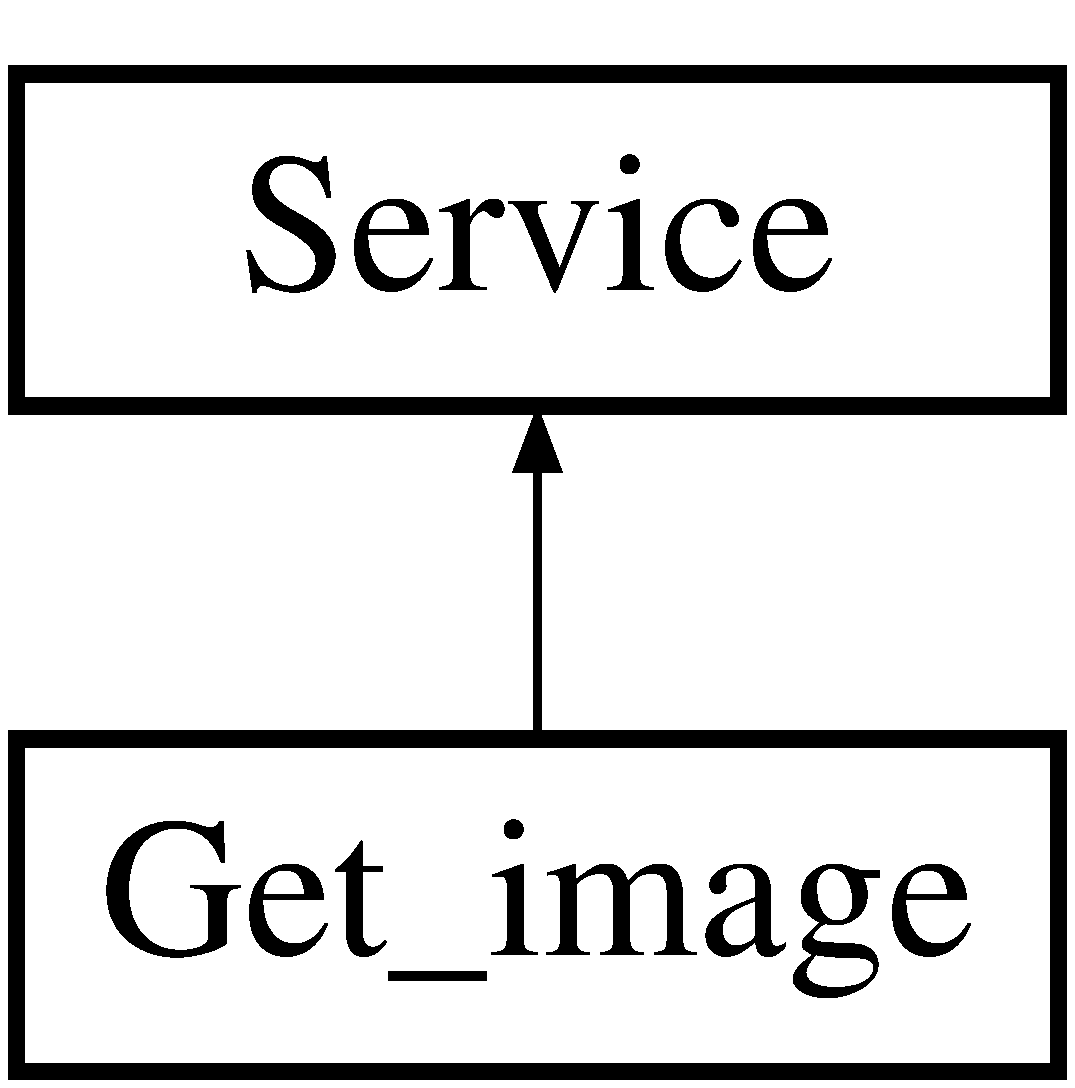
\includegraphics[height=2.000000cm]{class_get__image}
\end{center}
\end{figure}
\subsection*{Membri pubblici}
\begin{DoxyCompactItemize}
\item 
\hyperlink{class_get__image_a5517f5f85b538ebb63431448140a788a}{Get\-\_\-image} ()
\begin{DoxyCompactList}\small\item\em Costruttore di default della classe \hyperlink{class_get__image}{Get\-\_\-image}. \end{DoxyCompactList}\item 
\hyperlink{class_get__image_a1baaf0f15469480c90ed2c90a6a8b0dc}{Get\-\_\-image} (string name, string address, string port)
\begin{DoxyCompactList}\small\item\em Costruttore che inizializza l'istanza della classe \hyperlink{class_get__image}{Get\-\_\-image} con i parametri forniti. \end{DoxyCompactList}\item 
\hyperlink{class_get__image_a1e55c68de9f17dce123cb5bf1f6a9c6b}{Get\-\_\-image} (string name, string address, string port, string \hyperlink{class_get__image_a5a2f7a3384d879568383e61151f2bf11}{path})
\begin{DoxyCompactList}\small\item\em Costruttore che inizializza l'istanza della classe \hyperlink{class_get__image}{Get\-\_\-image} con i parametri forniti. \end{DoxyCompactList}\item 
\hyperlink{class_get__image_af742c8d21028f545c2d03afe3a468501}{Get\-\_\-image} (\hyperlink{struct_service__description}{Service\-\_\-description} $\ast$\hyperlink{class_service_a55e991ff18c0dceca202388a771283dc}{s\-\_\-description})
\begin{DoxyCompactList}\small\item\em Costruttore che inizializza la classe \hyperlink{class_get__image}{Get\-\_\-image} con le informazioni ottenute dalla descrizione del servizio. \end{DoxyCompactList}\item 
\hyperlink{class_get__image_ae1ca342b78c3df79faef72321c5728fa}{Get\-\_\-image} (\hyperlink{struct_service__description}{Service\-\_\-description} $\ast$\hyperlink{class_service_a55e991ff18c0dceca202388a771283dc}{s\-\_\-description}, string \hyperlink{class_get__image_a5a2f7a3384d879568383e61151f2bf11}{path})
\begin{DoxyCompactList}\small\item\em Costruttore che inizializza la classe \hyperlink{class_get__image}{Get\-\_\-image} con le informazioni ottenute dalla descrizione del servizio e imposta la directory di lavoro con il path fornito in ingresso. \end{DoxyCompactList}\item 
\hypertarget{class_get__image_a51a6a5acc16df05b182da40729e90cde}{virtual \hyperlink{class_get__image_a51a6a5acc16df05b182da40729e90cde}{$\sim$\-Get\-\_\-image} ()}\label{class_get__image_a51a6a5acc16df05b182da40729e90cde}

\begin{DoxyCompactList}\small\item\em Distruttore della classe \hyperlink{class_get__image}{Get\-\_\-image}. \end{DoxyCompactList}\item 
bool \hyperlink{class_get__image_ab133500614b9a2e7a1215a55f8729a6b}{execute} ()
\begin{DoxyCompactList}\small\item\em Compila il parametro di uscita del servizio con l'immagine richiesta dal chiamante (se presente). \end{DoxyCompactList}\end{DoxyCompactItemize}
\subsection*{Membri privati}
\begin{DoxyCompactItemize}
\item 
void \hyperlink{class_get__image_a01517b99c0d3c7ac9a7daaf3fa7fe4fd}{inizialize\-\_\-parameters} (string \hyperlink{class_get__image_a5a2f7a3384d879568383e61151f2bf11}{path})
\begin{DoxyCompactList}\small\item\em Inizializza l'istanza della classe \hyperlink{class_get__image}{Get\-\_\-image} (è chiamata da ogni costruttore). \end{DoxyCompactList}\end{DoxyCompactItemize}
\subsection*{Attributi privati}
\begin{DoxyCompactItemize}
\item 
\hypertarget{class_get__image_a5a2f7a3384d879568383e61151f2bf11}{string \hyperlink{class_get__image_a5a2f7a3384d879568383e61151f2bf11}{path}}\label{class_get__image_a5a2f7a3384d879568383e61151f2bf11}

\begin{DoxyCompactList}\small\item\em Directory di lavoro dello {\itshape Storage\-\_\-server} dove ricercare le immagini da fornire ai {\itshape Clients}. \end{DoxyCompactList}\end{DoxyCompactItemize}
\subsection*{Altri membri ereditati}


\subsection{Descrizione dettagliata}
Classe che fornisce al richiedente un'immagine presente sul server remoto. E' una classe derivate di {\ttfamily \hyperlink{class_service}{Service}}. 

Definizione alla linea 97 del file Get\-\_\-image.\-h.



\subsection{Documentazione dei costruttori e dei distruttori}
\hypertarget{class_get__image_a5517f5f85b538ebb63431448140a788a}{\index{Get\-\_\-image@{Get\-\_\-image}!Get\-\_\-image@{Get\-\_\-image}}
\index{Get\-\_\-image@{Get\-\_\-image}!Get_image@{Get\-\_\-image}}
\subsubsection[{Get\-\_\-image}]{\setlength{\rightskip}{0pt plus 5cm}Get\-\_\-image\-::\-Get\-\_\-image (
\begin{DoxyParamCaption}
{}
\end{DoxyParamCaption}
)}}\label{class_get__image_a5517f5f85b538ebb63431448140a788a}


Costruttore di default della classe \hyperlink{class_get__image}{Get\-\_\-image}. 

Costruttore di default della classe \hyperlink{class_get__image}{Get\-\_\-image}. Provoca l'inizializzazione dei parametri di ingresso e uscita del servizio e setta la directory di lavoro sulla directory default. 

Definizione alla linea 5 del file Get\-\_\-image.\-cpp.

\hypertarget{class_get__image_a1baaf0f15469480c90ed2c90a6a8b0dc}{\index{Get\-\_\-image@{Get\-\_\-image}!Get\-\_\-image@{Get\-\_\-image}}
\index{Get\-\_\-image@{Get\-\_\-image}!Get_image@{Get\-\_\-image}}
\subsubsection[{Get\-\_\-image}]{\setlength{\rightskip}{0pt plus 5cm}Get\-\_\-image\-::\-Get\-\_\-image (
\begin{DoxyParamCaption}
\item[{string}]{name, }
\item[{string}]{address, }
\item[{string}]{port}
\end{DoxyParamCaption}
)}}\label{class_get__image_a1baaf0f15469480c90ed2c90a6a8b0dc}


Costruttore che inizializza l'istanza della classe \hyperlink{class_get__image}{Get\-\_\-image} con i parametri forniti. 


\begin{DoxyParams}[1]{Parametri}
\mbox{\tt in}  & {\em name} & Nome da assegnare al servizio. \\
\hline
\mbox{\tt in}  & {\em address} & Indirizzo I\-P del service provider che fornisce il servizio. \\
\hline
\mbox{\tt in}  & {\em port} & Porta di ascolto del service provider che fornisce il servizio. Costruttore che inizializza l'istanza della classe \hyperlink{class_get__image}{Get\-\_\-image} con nome, indirizzo e porta forniti in ingresso, inizializza i parametri di ingresso e uscita del servizio e setta la directory di lavoro sulla directory default. \\
\hline
\end{DoxyParams}


Definizione alla linea 9 del file Get\-\_\-image.\-cpp.

\hypertarget{class_get__image_a1e55c68de9f17dce123cb5bf1f6a9c6b}{\index{Get\-\_\-image@{Get\-\_\-image}!Get\-\_\-image@{Get\-\_\-image}}
\index{Get\-\_\-image@{Get\-\_\-image}!Get_image@{Get\-\_\-image}}
\subsubsection[{Get\-\_\-image}]{\setlength{\rightskip}{0pt plus 5cm}Get\-\_\-image\-::\-Get\-\_\-image (
\begin{DoxyParamCaption}
\item[{string}]{name, }
\item[{string}]{address, }
\item[{string}]{port, }
\item[{string}]{path}
\end{DoxyParamCaption}
)}}\label{class_get__image_a1e55c68de9f17dce123cb5bf1f6a9c6b}


Costruttore che inizializza l'istanza della classe \hyperlink{class_get__image}{Get\-\_\-image} con i parametri forniti. 


\begin{DoxyParams}[1]{Parametri}
\mbox{\tt in}  & {\em name} & Nome da assegnare al servizio. \\
\hline
\mbox{\tt in}  & {\em address} & Indirizzo I\-P del service provider che fornisce il servizio. \\
\hline
\mbox{\tt in}  & {\em port} & Porta di ascolto del service provider che fornisce il servizio. \\
\hline
\mbox{\tt in}  & {\em path} & Directory di lavoro dove ricercare i files per creare la lista. Costruttore che inizializza l'istanza della classe \hyperlink{class_get__image}{Get\-\_\-image} con nome, indirizzo e porta forniti in ingresso, inizializza i parametri di ingresso e uscita del servizio e imposta la directory di lavoro con il path fornito in ingresso. \\
\hline
\end{DoxyParams}


Definizione alla linea 12 del file Get\-\_\-image.\-cpp.

\hypertarget{class_get__image_af742c8d21028f545c2d03afe3a468501}{\index{Get\-\_\-image@{Get\-\_\-image}!Get\-\_\-image@{Get\-\_\-image}}
\index{Get\-\_\-image@{Get\-\_\-image}!Get_image@{Get\-\_\-image}}
\subsubsection[{Get\-\_\-image}]{\setlength{\rightskip}{0pt plus 5cm}Get\-\_\-image\-::\-Get\-\_\-image (
\begin{DoxyParamCaption}
\item[{{\bf Service\-\_\-description} $\ast$}]{s\-\_\-description}
\end{DoxyParamCaption}
)}}\label{class_get__image_af742c8d21028f545c2d03afe3a468501}


Costruttore che inizializza la classe \hyperlink{class_get__image}{Get\-\_\-image} con le informazioni ottenute dalla descrizione del servizio. 


\begin{DoxyParams}[1]{Parametri}
\mbox{\tt in}  & {\em s\-\_\-description} & Descrizione del servizio. \\
\hline
\end{DoxyParams}


Definizione alla linea 15 del file Get\-\_\-image.\-cpp.

\hypertarget{class_get__image_ae1ca342b78c3df79faef72321c5728fa}{\index{Get\-\_\-image@{Get\-\_\-image}!Get\-\_\-image@{Get\-\_\-image}}
\index{Get\-\_\-image@{Get\-\_\-image}!Get_image@{Get\-\_\-image}}
\subsubsection[{Get\-\_\-image}]{\setlength{\rightskip}{0pt plus 5cm}Get\-\_\-image\-::\-Get\-\_\-image (
\begin{DoxyParamCaption}
\item[{{\bf Service\-\_\-description} $\ast$}]{s\-\_\-description, }
\item[{string}]{path}
\end{DoxyParamCaption}
)}}\label{class_get__image_ae1ca342b78c3df79faef72321c5728fa}


Costruttore che inizializza la classe \hyperlink{class_get__image}{Get\-\_\-image} con le informazioni ottenute dalla descrizione del servizio e imposta la directory di lavoro con il path fornito in ingresso. 


\begin{DoxyParams}[1]{Parametri}
\mbox{\tt in}  & {\em s\-\_\-description} & Descrizione del servizio. \\
\hline
\mbox{\tt in}  & {\em path} & Directory di lavoro dove ricercare i files per creare la lista. \\
\hline
\end{DoxyParams}


Definizione alla linea 21 del file Get\-\_\-image.\-cpp.



\subsection{Documentazione delle funzioni membro}
\hypertarget{class_get__image_ab133500614b9a2e7a1215a55f8729a6b}{\index{Get\-\_\-image@{Get\-\_\-image}!execute@{execute}}
\index{execute@{execute}!Get_image@{Get\-\_\-image}}
\subsubsection[{execute}]{\setlength{\rightskip}{0pt plus 5cm}bool Get\-\_\-image\-::execute (
\begin{DoxyParamCaption}
{}
\end{DoxyParamCaption}
)\hspace{0.3cm}{\ttfamily [virtual]}}}\label{class_get__image_ab133500614b9a2e7a1215a55f8729a6b}


Compila il parametro di uscita del servizio con l'immagine richiesta dal chiamante (se presente). 

\begin{DoxyReturn}{Restituisce}
Risultato dell'esecuzione, {\ttfamily true} in caso di successo e {\ttfamily false} altrimenti. 
\end{DoxyReturn}


Reimplementa \hyperlink{class_service}{Service}.



Definizione alla linea 39 del file Get\-\_\-image.\-cpp.

\hypertarget{class_get__image_a01517b99c0d3c7ac9a7daaf3fa7fe4fd}{\index{Get\-\_\-image@{Get\-\_\-image}!inizialize\-\_\-parameters@{inizialize\-\_\-parameters}}
\index{inizialize\-\_\-parameters@{inizialize\-\_\-parameters}!Get_image@{Get\-\_\-image}}
\subsubsection[{inizialize\-\_\-parameters}]{\setlength{\rightskip}{0pt plus 5cm}Get\-\_\-image\-::inizialize\-\_\-parameters (
\begin{DoxyParamCaption}
\item[{string}]{path}
\end{DoxyParamCaption}
)\hspace{0.3cm}{\ttfamily [private]}}}\label{class_get__image_a01517b99c0d3c7ac9a7daaf3fa7fe4fd}


Inizializza l'istanza della classe \hyperlink{class_get__image}{Get\-\_\-image} (è chiamata da ogni costruttore). 


\begin{DoxyParams}[1]{Parametri}
\mbox{\tt in}  & {\em path} & Directory di lavoro dove ricercare i files per creare la lista. Inizializza l'istanza della classe \hyperlink{class_get__image}{Get\-\_\-image} come segue\-: \begin{DoxyItemize}
\item genera un parametro in ingresso di tipo {\ttfamily string} che conterrà il nome dell'immagine da richiedere al server remoto \item genera un parametro in uscita di tipo {\itshape buffer} per l'immagine da inviare al {\itshape Client} \item crea la directory di lavoro del servizio se questa non esiste \end{DoxyItemize}
\\
\hline
\end{DoxyParams}


Definizione alla linea 30 del file Get\-\_\-image.\-cpp.



La documentazione per questa classe è stata generata a partire dai seguenti file\-:\begin{DoxyCompactItemize}
\item 
C\-:/\-Users/\-Matteo/\-Dropbox/\-Universita/\-Sistemi Operativi e Programmazione Distribuita/\-Progetto/\-Service\-\_\-\-Oriented\-\_\-\-Architecture/\-Sources/\-Application/\-Image\-\_\-storage\-\_\-server/\hyperlink{_get__image_8h}{Get\-\_\-image.\-h}\item 
C\-:/\-Users/\-Matteo/\-Dropbox/\-Universita/\-Sistemi Operativi e Programmazione Distribuita/\-Progetto/\-Service\-\_\-\-Oriented\-\_\-\-Architecture/\-Sources/\-Application/\-Image\-\_\-storage\-\_\-server/Get\-\_\-image.\-cpp\end{DoxyCompactItemize}

\hypertarget{class_get__list}{\section{Riferimenti per la classe Get\-\_\-list}
\label{class_get__list}\index{Get\-\_\-list@{Get\-\_\-list}}
}


Classe che fornisce la lista dei files presenti sul server remoto. E' una classe derivate di {\ttfamily \hyperlink{class_service}{Service}}.  




{\ttfamily \#include $<$Get\-\_\-list.\-h$>$}

Diagramma delle classi per Get\-\_\-list\begin{figure}[H]
\begin{center}
\leavevmode
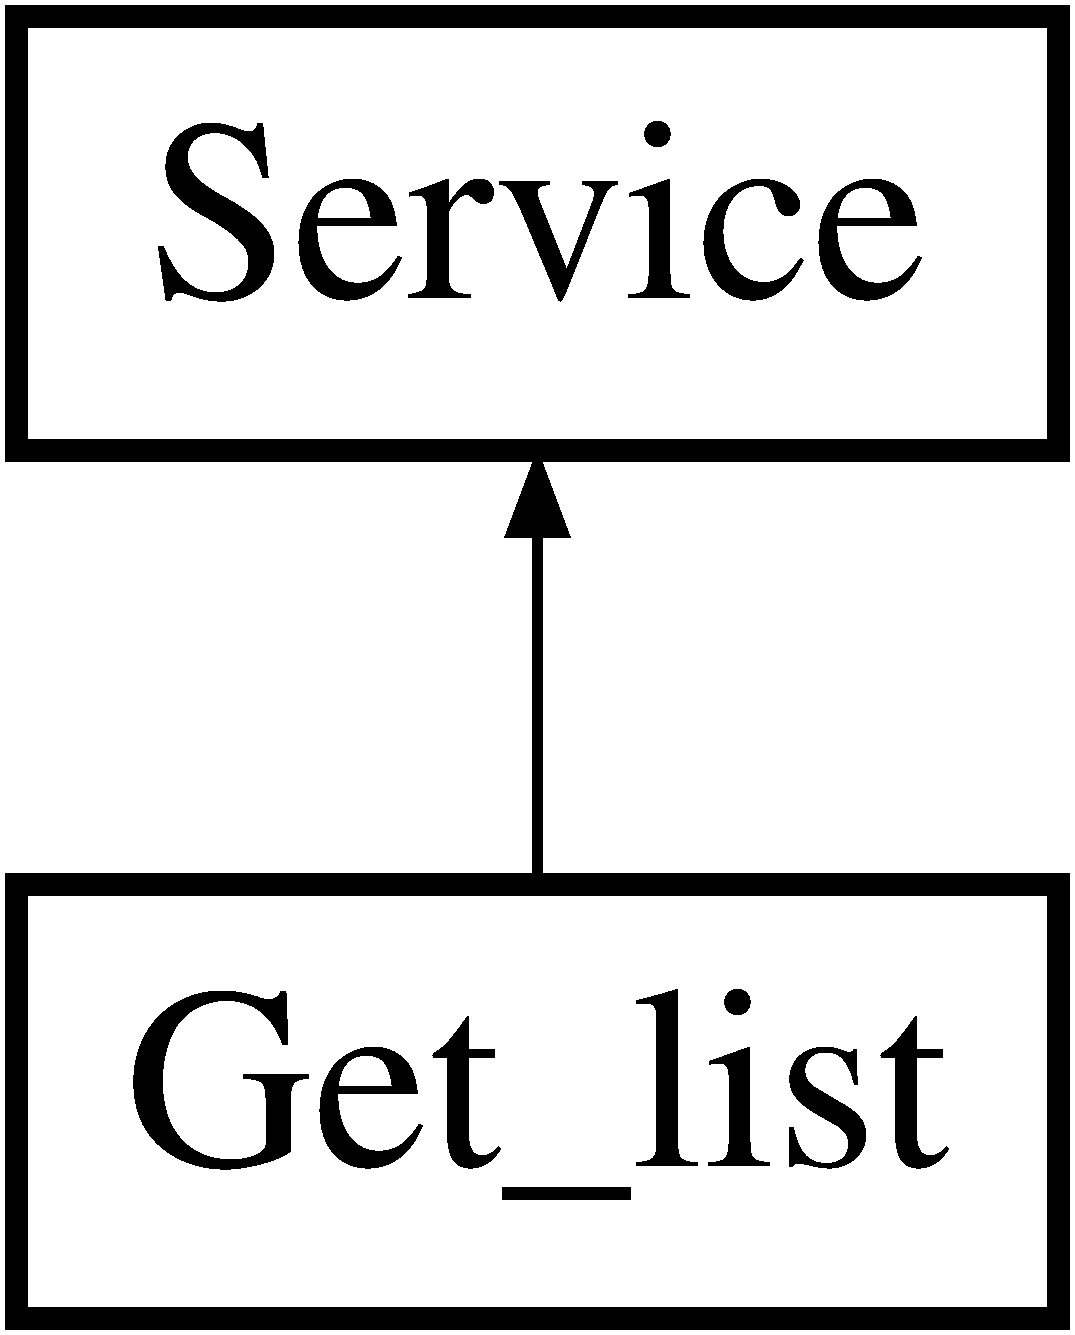
\includegraphics[height=2.000000cm]{class_get__list}
\end{center}
\end{figure}
\subsection*{Membri pubblici}
\begin{DoxyCompactItemize}
\item 
\hyperlink{class_get__list_ab76ae414df34e6cb71e0f5b52ca39c92}{Get\-\_\-list} ()
\begin{DoxyCompactList}\small\item\em Costruttore di default della classe \hyperlink{class_get__list}{Get\-\_\-list}. \end{DoxyCompactList}\item 
\hyperlink{class_get__list_a5eb8a30fb6f1a4c3190f889a3f87129b}{Get\-\_\-list} (string name, string address, string port)
\begin{DoxyCompactList}\small\item\em Costruttore che inizializza l'istanza della classe \hyperlink{class_get__list}{Get\-\_\-list} con i parametri forniti. \end{DoxyCompactList}\item 
\hyperlink{class_get__list_a252524419d25158e1115bec0d023c494}{Get\-\_\-list} (string name, string address, string port, string \hyperlink{class_get__list_a7880b35d31e6171ae53378d9d1d4afca}{path})
\begin{DoxyCompactList}\small\item\em Costruttore che inizializza l'istanza della classe \hyperlink{class_get__list}{Get\-\_\-list} con i parametri forniti. \end{DoxyCompactList}\item 
\hyperlink{class_get__list_a51bc5354d5a3ee2fd6598495725df152}{Get\-\_\-list} (\hyperlink{struct_service__description}{Service\-\_\-description} $\ast$\hyperlink{class_service_a55e991ff18c0dceca202388a771283dc}{s\-\_\-description})
\begin{DoxyCompactList}\small\item\em Costruttore che inizializza la classe \hyperlink{class_get__list}{Get\-\_\-list} con le informazioni ottenute dalla descrizione del servizio. \end{DoxyCompactList}\item 
\hyperlink{class_get__list_ab81f316f9deccbc40f1811cf1c06d718}{Get\-\_\-list} (\hyperlink{struct_service__description}{Service\-\_\-description} $\ast$\hyperlink{class_service_a55e991ff18c0dceca202388a771283dc}{s\-\_\-description}, string \hyperlink{class_get__list_a7880b35d31e6171ae53378d9d1d4afca}{path})
\begin{DoxyCompactList}\small\item\em Costruttore che inizializza la classe \hyperlink{class_get__list}{Get\-\_\-list} con le informazioni ottenute dalla descrizione del servizio e imposta la directory di lavoro con il path fornito in ingresso. \end{DoxyCompactList}\item 
\hypertarget{class_get__list_ad4b5aab752d75ec562db1b8ced98eb76}{virtual \hyperlink{class_get__list_ad4b5aab752d75ec562db1b8ced98eb76}{$\sim$\-Get\-\_\-list} ()}\label{class_get__list_ad4b5aab752d75ec562db1b8ced98eb76}

\begin{DoxyCompactList}\small\item\em Distruttore della classe \hyperlink{class_get__list}{Get\-\_\-list}. \end{DoxyCompactList}\item 
bool \hyperlink{class_get__list_aa7304342c475406fdc5f6fc36540c309}{execute} ()
\begin{DoxyCompactList}\small\item\em Genera la lista dei files presenti nella directory di lavoro del {\itshape Server} e con questa compila il parametro di uscita del servizio. \end{DoxyCompactList}\end{DoxyCompactItemize}
\subsection*{Membri privati}
\begin{DoxyCompactItemize}
\item 
void \hyperlink{class_get__list_ac69fa4b93dbc29ee9ef48f6ad7042daa}{inizialize\-\_\-parameters} (string \hyperlink{class_get__list_a7880b35d31e6171ae53378d9d1d4afca}{path})
\begin{DoxyCompactList}\small\item\em Inizializza l'istanza della classe \hyperlink{class_get__list}{Get\-\_\-list} (è chiamata da ogni costruttore). \end{DoxyCompactList}\end{DoxyCompactItemize}
\subsection*{Attributi privati}
\begin{DoxyCompactItemize}
\item 
\hypertarget{class_get__list_a7880b35d31e6171ae53378d9d1d4afca}{string \hyperlink{class_get__list_a7880b35d31e6171ae53378d9d1d4afca}{path}}\label{class_get__list_a7880b35d31e6171ae53378d9d1d4afca}

\begin{DoxyCompactList}\small\item\em Directory di lavoro dello {\itshape Storage\-\_\-server} dove ricercare le immagini con cui creare la lista. \end{DoxyCompactList}\end{DoxyCompactItemize}
\subsection*{Altri membri ereditati}


\subsection{Descrizione dettagliata}
Classe che fornisce la lista dei files presenti sul server remoto. E' una classe derivate di {\ttfamily \hyperlink{class_service}{Service}}. 

Definizione alla linea 96 del file Get\-\_\-list.\-h.



\subsection{Documentazione dei costruttori e dei distruttori}
\hypertarget{class_get__list_ab76ae414df34e6cb71e0f5b52ca39c92}{\index{Get\-\_\-list@{Get\-\_\-list}!Get\-\_\-list@{Get\-\_\-list}}
\index{Get\-\_\-list@{Get\-\_\-list}!Get_list@{Get\-\_\-list}}
\subsubsection[{Get\-\_\-list}]{\setlength{\rightskip}{0pt plus 5cm}Get\-\_\-list\-::\-Get\-\_\-list (
\begin{DoxyParamCaption}
{}
\end{DoxyParamCaption}
)}}\label{class_get__list_ab76ae414df34e6cb71e0f5b52ca39c92}


Costruttore di default della classe \hyperlink{class_get__list}{Get\-\_\-list}. 

Costruttore di default della classe \hyperlink{class_get__list}{Get\-\_\-list}. Provoca l'inizializzazione dei parametri di ingresso e uscita del servizio e setta la directory di lavoro sulla directory default. 

Definizione alla linea 5 del file Get\-\_\-list.\-cpp.

\hypertarget{class_get__list_a5eb8a30fb6f1a4c3190f889a3f87129b}{\index{Get\-\_\-list@{Get\-\_\-list}!Get\-\_\-list@{Get\-\_\-list}}
\index{Get\-\_\-list@{Get\-\_\-list}!Get_list@{Get\-\_\-list}}
\subsubsection[{Get\-\_\-list}]{\setlength{\rightskip}{0pt plus 5cm}Get\-\_\-list\-::\-Get\-\_\-list (
\begin{DoxyParamCaption}
\item[{string}]{name, }
\item[{string}]{address, }
\item[{string}]{port}
\end{DoxyParamCaption}
)}}\label{class_get__list_a5eb8a30fb6f1a4c3190f889a3f87129b}


Costruttore che inizializza l'istanza della classe \hyperlink{class_get__list}{Get\-\_\-list} con i parametri forniti. 


\begin{DoxyParams}[1]{Parametri}
\mbox{\tt in}  & {\em name} & Nome da assegnare al servizio. \\
\hline
\mbox{\tt in}  & {\em address} & Indirizzo I\-P del service provider che fornisce il servizio. \\
\hline
\mbox{\tt in}  & {\em port} & Porta di ascolto del service provider che fornisce il servizio. Costruttore che inizializza l'istanza della classe \hyperlink{class_get__list}{Get\-\_\-list} con nome, indirizzo e porta forniti in ingresso, inizializza i parametri di ingresso e uscita del servizio e setta la directory di lavoro sulla directory default. \\
\hline
\end{DoxyParams}


Definizione alla linea 9 del file Get\-\_\-list.\-cpp.

\hypertarget{class_get__list_a252524419d25158e1115bec0d023c494}{\index{Get\-\_\-list@{Get\-\_\-list}!Get\-\_\-list@{Get\-\_\-list}}
\index{Get\-\_\-list@{Get\-\_\-list}!Get_list@{Get\-\_\-list}}
\subsubsection[{Get\-\_\-list}]{\setlength{\rightskip}{0pt plus 5cm}Get\-\_\-list\-::\-Get\-\_\-list (
\begin{DoxyParamCaption}
\item[{string}]{name, }
\item[{string}]{address, }
\item[{string}]{port, }
\item[{string}]{path}
\end{DoxyParamCaption}
)}}\label{class_get__list_a252524419d25158e1115bec0d023c494}


Costruttore che inizializza l'istanza della classe \hyperlink{class_get__list}{Get\-\_\-list} con i parametri forniti. 


\begin{DoxyParams}[1]{Parametri}
\mbox{\tt in}  & {\em name} & Nome da assegnare al servizio. \\
\hline
\mbox{\tt in}  & {\em address} & Indirizzo I\-P del service provider che fornisce il servizio. \\
\hline
\mbox{\tt in}  & {\em port} & Porta di ascolto del service provider che fornisce il servizio. \\
\hline
\mbox{\tt in}  & {\em path} & Directory di lavoro dove ricercare i files per creare la lista. Costruttore che inizializza l'istanza della classe \hyperlink{class_get__list}{Get\-\_\-list} con nome, indirizzo e porta forniti in ingresso, inizializza i parametri di ingresso e uscita del servizio e imposta la directory di lavoro con il path fornito in ingresso. \\
\hline
\end{DoxyParams}


Definizione alla linea 12 del file Get\-\_\-list.\-cpp.

\hypertarget{class_get__list_a51bc5354d5a3ee2fd6598495725df152}{\index{Get\-\_\-list@{Get\-\_\-list}!Get\-\_\-list@{Get\-\_\-list}}
\index{Get\-\_\-list@{Get\-\_\-list}!Get_list@{Get\-\_\-list}}
\subsubsection[{Get\-\_\-list}]{\setlength{\rightskip}{0pt plus 5cm}Get\-\_\-list\-::\-Get\-\_\-list (
\begin{DoxyParamCaption}
\item[{{\bf Service\-\_\-description} $\ast$}]{s\-\_\-description}
\end{DoxyParamCaption}
)}}\label{class_get__list_a51bc5354d5a3ee2fd6598495725df152}


Costruttore che inizializza la classe \hyperlink{class_get__list}{Get\-\_\-list} con le informazioni ottenute dalla descrizione del servizio. 


\begin{DoxyParams}[1]{Parametri}
\mbox{\tt in}  & {\em s\-\_\-description} & Descrizione del servizio. \\
\hline
\end{DoxyParams}


Definizione alla linea 15 del file Get\-\_\-list.\-cpp.

\hypertarget{class_get__list_ab81f316f9deccbc40f1811cf1c06d718}{\index{Get\-\_\-list@{Get\-\_\-list}!Get\-\_\-list@{Get\-\_\-list}}
\index{Get\-\_\-list@{Get\-\_\-list}!Get_list@{Get\-\_\-list}}
\subsubsection[{Get\-\_\-list}]{\setlength{\rightskip}{0pt plus 5cm}Get\-\_\-list\-::\-Get\-\_\-list (
\begin{DoxyParamCaption}
\item[{{\bf Service\-\_\-description} $\ast$}]{s\-\_\-description, }
\item[{string}]{path}
\end{DoxyParamCaption}
)}}\label{class_get__list_ab81f316f9deccbc40f1811cf1c06d718}


Costruttore che inizializza la classe \hyperlink{class_get__list}{Get\-\_\-list} con le informazioni ottenute dalla descrizione del servizio e imposta la directory di lavoro con il path fornito in ingresso. 


\begin{DoxyParams}[1]{Parametri}
\mbox{\tt in}  & {\em s\-\_\-description} & Descrizione del servizio. \\
\hline
\mbox{\tt in}  & {\em path} & Directory di lavoro dove ricercare i files per creare la lista. \\
\hline
\end{DoxyParams}


Definizione alla linea 21 del file Get\-\_\-list.\-cpp.



\subsection{Documentazione delle funzioni membro}
\hypertarget{class_get__list_aa7304342c475406fdc5f6fc36540c309}{\index{Get\-\_\-list@{Get\-\_\-list}!execute@{execute}}
\index{execute@{execute}!Get_list@{Get\-\_\-list}}
\subsubsection[{execute}]{\setlength{\rightskip}{0pt plus 5cm}bool Get\-\_\-list\-::execute (
\begin{DoxyParamCaption}
{}
\end{DoxyParamCaption}
)\hspace{0.3cm}{\ttfamily [virtual]}}}\label{class_get__list_aa7304342c475406fdc5f6fc36540c309}


Genera la lista dei files presenti nella directory di lavoro del {\itshape Server} e con questa compila il parametro di uscita del servizio. 

\begin{DoxyReturn}{Restituisce}
Risultato dell'esecuzione, {\ttfamily true} in caso di successo e {\ttfamily false} altrimenti. 
\end{DoxyReturn}


Reimplementa \hyperlink{class_service}{Service}.



Definizione alla linea 38 del file Get\-\_\-list.\-cpp.

\hypertarget{class_get__list_ac69fa4b93dbc29ee9ef48f6ad7042daa}{\index{Get\-\_\-list@{Get\-\_\-list}!inizialize\-\_\-parameters@{inizialize\-\_\-parameters}}
\index{inizialize\-\_\-parameters@{inizialize\-\_\-parameters}!Get_list@{Get\-\_\-list}}
\subsubsection[{inizialize\-\_\-parameters}]{\setlength{\rightskip}{0pt plus 5cm}Get\-\_\-list\-::inizialize\-\_\-parameters (
\begin{DoxyParamCaption}
\item[{string}]{path}
\end{DoxyParamCaption}
)\hspace{0.3cm}{\ttfamily [private]}}}\label{class_get__list_ac69fa4b93dbc29ee9ef48f6ad7042daa}


Inizializza l'istanza della classe \hyperlink{class_get__list}{Get\-\_\-list} (è chiamata da ogni costruttore). 


\begin{DoxyParams}[1]{Parametri}
\mbox{\tt in}  & {\em path} & Directory di lavoro dove ricercare i files per creare la lista. Inizializza l'istanza della classe \hyperlink{class_get__list}{Get\-\_\-list} come segue\-: \begin{DoxyItemize}
\item genera un parametro in uscita di tipo {\ttfamily string} che conterrà la lista dei files presenti sul server remoto \item crea la directory di lavoro del servizio se questa non esiste \end{DoxyItemize}
\\
\hline
\end{DoxyParams}


Definizione alla linea 30 del file Get\-\_\-list.\-cpp.



La documentazione per questa classe è stata generata a partire dai seguenti file\-:\begin{DoxyCompactItemize}
\item 
C\-:/\-Users/\-Matteo/\-Dropbox/\-Universita/\-Sistemi Operativi e Programmazione Distribuita/\-Progetto/\-Service\-\_\-\-Oriented\-\_\-\-Architecture/\-Sources/\-Application/\-Image\-\_\-storage\-\_\-server/\hyperlink{_get__list_8h}{Get\-\_\-list.\-h}\item 
C\-:/\-Users/\-Matteo/\-Dropbox/\-Universita/\-Sistemi Operativi e Programmazione Distribuita/\-Progetto/\-Service\-\_\-\-Oriented\-\_\-\-Architecture/\-Sources/\-Application/\-Image\-\_\-storage\-\_\-server/Get\-\_\-list.\-cpp\end{DoxyCompactItemize}

\hypertarget{class_horizontal__flip__image}{\section{Riferimenti per la classe Horizontal\-\_\-flip\-\_\-image}
\label{class_horizontal__flip__image}\index{Horizontal\-\_\-flip\-\_\-image@{Horizontal\-\_\-flip\-\_\-image}}
}


Classe che fornisce il servizio di riflessione di un immagine. E' una classe derivate di {\ttfamily \hyperlink{class_service}{Service}}.  




{\ttfamily \#include $<$Horizontal\-\_\-flip\-\_\-image.\-h$>$}

Diagramma delle classi per Horizontal\-\_\-flip\-\_\-image\begin{figure}[H]
\begin{center}
\leavevmode
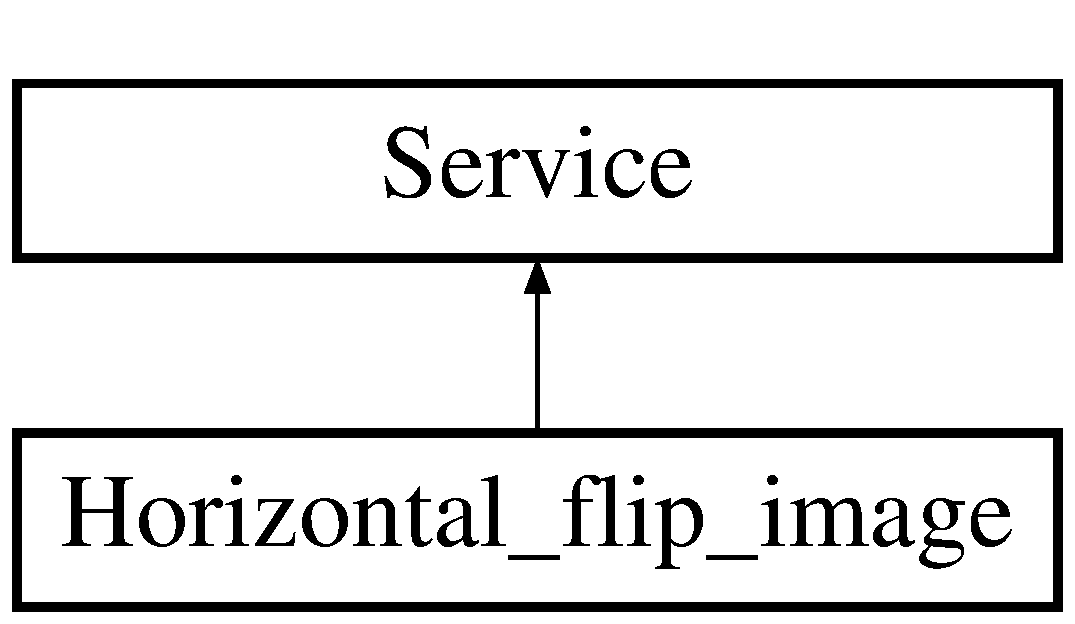
\includegraphics[height=2.000000cm]{class_horizontal__flip__image}
\end{center}
\end{figure}
\subsection*{Membri pubblici}
\begin{DoxyCompactItemize}
\item 
\hyperlink{class_horizontal__flip__image_a948547064eeea73d824b899a99d98803}{Horizontal\-\_\-flip\-\_\-image} ()
\begin{DoxyCompactList}\small\item\em Costruttore di default della classe \hyperlink{class_horizontal__flip__image}{Horizontal\-\_\-flip\-\_\-image}. \end{DoxyCompactList}\item 
\hyperlink{class_horizontal__flip__image_a168239ec414f64df44d857dc58179851}{Horizontal\-\_\-flip\-\_\-image} (string name, string address, string port)
\begin{DoxyCompactList}\small\item\em Costruttore che inizializza l'istanza della classe \hyperlink{class_horizontal__flip__image}{Horizontal\-\_\-flip\-\_\-image} con i parametri forniti. \end{DoxyCompactList}\item 
\hyperlink{class_horizontal__flip__image_a17276cff85b5be92f368e39d7289be4b}{Horizontal\-\_\-flip\-\_\-image} (string name, string address, string port, string \hyperlink{class_horizontal__flip__image_a56deaa91c8efad258a778d4fece9c81b}{path})
\begin{DoxyCompactList}\small\item\em Costruttore che inizializza l'istanza della classe \hyperlink{class_horizontal__flip__image}{Horizontal\-\_\-flip\-\_\-image} con i parametri forniti. \end{DoxyCompactList}\item 
\hyperlink{class_horizontal__flip__image_a659aa882c8eb312880807c6cda07bf06}{Horizontal\-\_\-flip\-\_\-image} (\hyperlink{struct_service__description}{Service\-\_\-description} $\ast$\hyperlink{class_service_a55e991ff18c0dceca202388a771283dc}{s\-\_\-description})
\begin{DoxyCompactList}\small\item\em Costruttore che inizializza la classe \hyperlink{class_horizontal__flip__image}{Horizontal\-\_\-flip\-\_\-image} con le informazioni ottenute dalla descrizione del servizio. \end{DoxyCompactList}\item 
\hyperlink{class_horizontal__flip__image_a3421937ee79069dd965b01e21c0191b4}{Horizontal\-\_\-flip\-\_\-image} (\hyperlink{struct_service__description}{Service\-\_\-description} $\ast$\hyperlink{class_service_a55e991ff18c0dceca202388a771283dc}{s\-\_\-description}, string \hyperlink{class_horizontal__flip__image_a56deaa91c8efad258a778d4fece9c81b}{path})
\begin{DoxyCompactList}\small\item\em Costruttore che inizializza la classe \hyperlink{class_horizontal__flip__image}{Horizontal\-\_\-flip\-\_\-image} con le informazioni ottenute dalla descrizione del servizio e imposta la directory di lavoro con il path fornito in ingresso. \end{DoxyCompactList}\item 
\hypertarget{class_horizontal__flip__image_ab584c001738909be6f95c4b40295b924}{virtual \hyperlink{class_horizontal__flip__image_ab584c001738909be6f95c4b40295b924}{$\sim$\-Horizontal\-\_\-flip\-\_\-image} ()}\label{class_horizontal__flip__image_ab584c001738909be6f95c4b40295b924}

\begin{DoxyCompactList}\small\item\em Distruttore della classe \hyperlink{class_horizontal__flip__image}{Horizontal\-\_\-flip\-\_\-image}. \end{DoxyCompactList}\item 
bool \hyperlink{class_horizontal__flip__image_a938221e0bcaa7331d01444c77366339d}{execute} ()
\begin{DoxyCompactList}\small\item\em Funzione che espleta il servizio di riflessione dell'immagine. \end{DoxyCompactList}\end{DoxyCompactItemize}
\subsection*{Membri privati}
\begin{DoxyCompactItemize}
\item 
void \hyperlink{class_horizontal__flip__image_a19887934b05b36f2b3603535e5cac691}{inizialize\-\_\-parameters} (string \hyperlink{class_horizontal__flip__image_a56deaa91c8efad258a778d4fece9c81b}{path})
\begin{DoxyCompactList}\small\item\em Inizializza l'istanza della classe \hyperlink{class_horizontal__flip__image}{Horizontal\-\_\-flip\-\_\-image} (è chiamata da ogni costruttore). \end{DoxyCompactList}\end{DoxyCompactItemize}
\subsection*{Attributi privati}
\begin{DoxyCompactItemize}
\item 
\hypertarget{class_horizontal__flip__image_a56deaa91c8efad258a778d4fece9c81b}{string \hyperlink{class_horizontal__flip__image_a56deaa91c8efad258a778d4fece9c81b}{path}}\label{class_horizontal__flip__image_a56deaa91c8efad258a778d4fece9c81b}

\begin{DoxyCompactList}\small\item\em Directory di lavoro dove salvare i risultati temporanei (immagini sorgente e risultato della riflessione). \end{DoxyCompactList}\end{DoxyCompactItemize}
\subsection*{Altri membri ereditati}


\subsection{Descrizione dettagliata}
Classe che fornisce il servizio di riflessione di un immagine. E' una classe derivate di {\ttfamily \hyperlink{class_service}{Service}}. 

Definizione alla linea 113 del file Horizontal\-\_\-flip\-\_\-image.\-h.



\subsection{Documentazione dei costruttori e dei distruttori}
\hypertarget{class_horizontal__flip__image_a948547064eeea73d824b899a99d98803}{\index{Horizontal\-\_\-flip\-\_\-image@{Horizontal\-\_\-flip\-\_\-image}!Horizontal\-\_\-flip\-\_\-image@{Horizontal\-\_\-flip\-\_\-image}}
\index{Horizontal\-\_\-flip\-\_\-image@{Horizontal\-\_\-flip\-\_\-image}!Horizontal_flip_image@{Horizontal\-\_\-flip\-\_\-image}}
\subsubsection[{Horizontal\-\_\-flip\-\_\-image}]{\setlength{\rightskip}{0pt plus 5cm}Horizontal\-\_\-flip\-\_\-image\-::\-Horizontal\-\_\-flip\-\_\-image (
\begin{DoxyParamCaption}
{}
\end{DoxyParamCaption}
)}}\label{class_horizontal__flip__image_a948547064eeea73d824b899a99d98803}


Costruttore di default della classe \hyperlink{class_horizontal__flip__image}{Horizontal\-\_\-flip\-\_\-image}. 

Costruttore di default della classe \hyperlink{class_horizontal__flip__image}{Horizontal\-\_\-flip\-\_\-image}. Provoca l'inizializzazione dei parametri di ingresso e uscita del servizio e setta la directory di lavoro sulla directory default. 

Definizione alla linea 5 del file Horizontal\-\_\-flip\-\_\-image.\-cpp.

\hypertarget{class_horizontal__flip__image_a168239ec414f64df44d857dc58179851}{\index{Horizontal\-\_\-flip\-\_\-image@{Horizontal\-\_\-flip\-\_\-image}!Horizontal\-\_\-flip\-\_\-image@{Horizontal\-\_\-flip\-\_\-image}}
\index{Horizontal\-\_\-flip\-\_\-image@{Horizontal\-\_\-flip\-\_\-image}!Horizontal_flip_image@{Horizontal\-\_\-flip\-\_\-image}}
\subsubsection[{Horizontal\-\_\-flip\-\_\-image}]{\setlength{\rightskip}{0pt plus 5cm}Horizontal\-\_\-flip\-\_\-image\-::\-Horizontal\-\_\-flip\-\_\-image (
\begin{DoxyParamCaption}
\item[{string}]{name, }
\item[{string}]{address, }
\item[{string}]{port}
\end{DoxyParamCaption}
)}}\label{class_horizontal__flip__image_a168239ec414f64df44d857dc58179851}


Costruttore che inizializza l'istanza della classe \hyperlink{class_horizontal__flip__image}{Horizontal\-\_\-flip\-\_\-image} con i parametri forniti. 


\begin{DoxyParams}[1]{Parametri}
\mbox{\tt in}  & {\em name} & Nome da assegnare al servizio. \\
\hline
\mbox{\tt in}  & {\em address} & Indirizzo I\-P del service provider che fornisce il servizio. \\
\hline
\mbox{\tt in}  & {\em port} & Porta di ascolto del service provider che fornisce il servizio. Costruttore che inizializza l'istanza della classe \hyperlink{class_horizontal__flip__image}{Horizontal\-\_\-flip\-\_\-image} con nome, indirizzo e porta forniti in ingresso, inizializza i parametri di ingresso e uscita del servizio e setta la directory di lavoro sulla directory default. \\
\hline
\end{DoxyParams}


Definizione alla linea 9 del file Horizontal\-\_\-flip\-\_\-image.\-cpp.

\hypertarget{class_horizontal__flip__image_a17276cff85b5be92f368e39d7289be4b}{\index{Horizontal\-\_\-flip\-\_\-image@{Horizontal\-\_\-flip\-\_\-image}!Horizontal\-\_\-flip\-\_\-image@{Horizontal\-\_\-flip\-\_\-image}}
\index{Horizontal\-\_\-flip\-\_\-image@{Horizontal\-\_\-flip\-\_\-image}!Horizontal_flip_image@{Horizontal\-\_\-flip\-\_\-image}}
\subsubsection[{Horizontal\-\_\-flip\-\_\-image}]{\setlength{\rightskip}{0pt plus 5cm}Horizontal\-\_\-flip\-\_\-image\-::\-Horizontal\-\_\-flip\-\_\-image (
\begin{DoxyParamCaption}
\item[{string}]{name, }
\item[{string}]{address, }
\item[{string}]{port, }
\item[{string}]{path}
\end{DoxyParamCaption}
)}}\label{class_horizontal__flip__image_a17276cff85b5be92f368e39d7289be4b}


Costruttore che inizializza l'istanza della classe \hyperlink{class_horizontal__flip__image}{Horizontal\-\_\-flip\-\_\-image} con i parametri forniti. 


\begin{DoxyParams}[1]{Parametri}
\mbox{\tt in}  & {\em name} & Nome da assegnare al servizio. \\
\hline
\mbox{\tt in}  & {\em address} & Indirizzo I\-P del service provider che fornisce il servizio. \\
\hline
\mbox{\tt in}  & {\em port} & Porta di ascolto del service provider che fornisce il servizio. \\
\hline
\mbox{\tt in}  & {\em path} & Directory di lavoro da assegnare al servizio dove salvare i files temporanei. Costruttore che inizializza l'istanza della classe \hyperlink{class_horizontal__flip__image}{Horizontal\-\_\-flip\-\_\-image} con nome, indirizzo e porta forniti in ingresso, inizializza i parametri di ingresso e uscita del servizio e imposta la directory di lavoro con il path fornito in ingresso. \\
\hline
\end{DoxyParams}


Definizione alla linea 12 del file Horizontal\-\_\-flip\-\_\-image.\-cpp.

\hypertarget{class_horizontal__flip__image_a659aa882c8eb312880807c6cda07bf06}{\index{Horizontal\-\_\-flip\-\_\-image@{Horizontal\-\_\-flip\-\_\-image}!Horizontal\-\_\-flip\-\_\-image@{Horizontal\-\_\-flip\-\_\-image}}
\index{Horizontal\-\_\-flip\-\_\-image@{Horizontal\-\_\-flip\-\_\-image}!Horizontal_flip_image@{Horizontal\-\_\-flip\-\_\-image}}
\subsubsection[{Horizontal\-\_\-flip\-\_\-image}]{\setlength{\rightskip}{0pt plus 5cm}Horizontal\-\_\-flip\-\_\-image\-::\-Horizontal\-\_\-flip\-\_\-image (
\begin{DoxyParamCaption}
\item[{{\bf Service\-\_\-description} $\ast$}]{s\-\_\-description}
\end{DoxyParamCaption}
)}}\label{class_horizontal__flip__image_a659aa882c8eb312880807c6cda07bf06}


Costruttore che inizializza la classe \hyperlink{class_horizontal__flip__image}{Horizontal\-\_\-flip\-\_\-image} con le informazioni ottenute dalla descrizione del servizio. 


\begin{DoxyParams}[1]{Parametri}
\mbox{\tt in}  & {\em s\-\_\-description} & Descrizione del servizio. \\
\hline
\end{DoxyParams}


Definizione alla linea 15 del file Horizontal\-\_\-flip\-\_\-image.\-cpp.

\hypertarget{class_horizontal__flip__image_a3421937ee79069dd965b01e21c0191b4}{\index{Horizontal\-\_\-flip\-\_\-image@{Horizontal\-\_\-flip\-\_\-image}!Horizontal\-\_\-flip\-\_\-image@{Horizontal\-\_\-flip\-\_\-image}}
\index{Horizontal\-\_\-flip\-\_\-image@{Horizontal\-\_\-flip\-\_\-image}!Horizontal_flip_image@{Horizontal\-\_\-flip\-\_\-image}}
\subsubsection[{Horizontal\-\_\-flip\-\_\-image}]{\setlength{\rightskip}{0pt plus 5cm}Horizontal\-\_\-flip\-\_\-image\-::\-Horizontal\-\_\-flip\-\_\-image (
\begin{DoxyParamCaption}
\item[{{\bf Service\-\_\-description} $\ast$}]{s\-\_\-description, }
\item[{string}]{path}
\end{DoxyParamCaption}
)}}\label{class_horizontal__flip__image_a3421937ee79069dd965b01e21c0191b4}


Costruttore che inizializza la classe \hyperlink{class_horizontal__flip__image}{Horizontal\-\_\-flip\-\_\-image} con le informazioni ottenute dalla descrizione del servizio e imposta la directory di lavoro con il path fornito in ingresso. 


\begin{DoxyParams}[1]{Parametri}
\mbox{\tt in}  & {\em s\-\_\-description} & Descrizione del servizio. \\
\hline
\mbox{\tt in}  & {\em path} & Directory di lavoro da assegnare al servizio dove salvare i files temporanei. \\
\hline
\end{DoxyParams}


Definizione alla linea 21 del file Horizontal\-\_\-flip\-\_\-image.\-cpp.



\subsection{Documentazione delle funzioni membro}
\hypertarget{class_horizontal__flip__image_a938221e0bcaa7331d01444c77366339d}{\index{Horizontal\-\_\-flip\-\_\-image@{Horizontal\-\_\-flip\-\_\-image}!execute@{execute}}
\index{execute@{execute}!Horizontal_flip_image@{Horizontal\-\_\-flip\-\_\-image}}
\subsubsection[{execute}]{\setlength{\rightskip}{0pt plus 5cm}bool Horizontal\-\_\-flip\-\_\-image\-::execute (
\begin{DoxyParamCaption}
{}
\end{DoxyParamCaption}
)\hspace{0.3cm}{\ttfamily [virtual]}}}\label{class_horizontal__flip__image_a938221e0bcaa7331d01444c77366339d}


Funzione che espleta il servizio di riflessione dell'immagine. 

\begin{DoxyReturn}{Restituisce}
Risultato dell'esecuzione, {\ttfamily true} in caso di successo e {\ttfamily false} altrimenti. Il servizio di riflessione viene effettuato come segue\-: \begin{DoxyItemize}
\item genera nella directory di lavoro l'immagine da elaborare a partire dal parametro {\ttfamily buffer} in ingresso al servizio \item vi applica l'operatore di riflessione ottenendo una nuova immagine (da ritornare al chiamante) \item compila il parametro di uscita del servizio (di tipo {\itshape buffer}) con i dati dell'immagine riflessa \item se {\itshape R\-E\-M\-O\-V\-E\-\_\-\-I\-M\-A\-G\-E\-S} è impostato a {\ttfamily true}, rimuove le due immagini appena create (ormai inutili) dalla directory di lavoro \end{DoxyItemize}

\end{DoxyReturn}


Reimplementa \hyperlink{class_service}{Service}.



Definizione alla linea 39 del file Horizontal\-\_\-flip\-\_\-image.\-cpp.

\hypertarget{class_horizontal__flip__image_a19887934b05b36f2b3603535e5cac691}{\index{Horizontal\-\_\-flip\-\_\-image@{Horizontal\-\_\-flip\-\_\-image}!inizialize\-\_\-parameters@{inizialize\-\_\-parameters}}
\index{inizialize\-\_\-parameters@{inizialize\-\_\-parameters}!Horizontal_flip_image@{Horizontal\-\_\-flip\-\_\-image}}
\subsubsection[{inizialize\-\_\-parameters}]{\setlength{\rightskip}{0pt plus 5cm}Horizontal\-\_\-flip\-\_\-image\-::inizialize\-\_\-parameters (
\begin{DoxyParamCaption}
\item[{string}]{path}
\end{DoxyParamCaption}
)\hspace{0.3cm}{\ttfamily [private]}}}\label{class_horizontal__flip__image_a19887934b05b36f2b3603535e5cac691}


Inizializza l'istanza della classe \hyperlink{class_horizontal__flip__image}{Horizontal\-\_\-flip\-\_\-image} (è chiamata da ogni costruttore). 


\begin{DoxyParams}[1]{Parametri}
\mbox{\tt in}  & {\em path} & Directory di lavoro da assegnare al servizio dove salvare i files temporanei. Inizializza l'istanza della classe \hyperlink{class_horizontal__flip__image}{Horizontal\-\_\-flip\-\_\-image} come segue\-: \begin{DoxyItemize}
\item genera un parametro in ingresso di tipo {\ttfamily buffer} atto a mantenere le informazioni relative all'immagine da elaborare \item genera un parametro in uscita di tipo {\itshape buffer} per l'immagine riflessa \item crea la directory di lavoro del servizio se questa non esiste \end{DoxyItemize}
\\
\hline
\end{DoxyParams}


Definizione alla linea 30 del file Horizontal\-\_\-flip\-\_\-image.\-cpp.



La documentazione per questa classe è stata generata a partire dai seguenti file\-:\begin{DoxyCompactItemize}
\item 
C\-:/\-Users/\-Matteo/\-Dropbox/\-Universita/\-Sistemi Operativi e Programmazione Distribuita/\-Progetto/\-Service\-\_\-\-Oriented\-\_\-\-Architecture/\-Sources/\-Application/\-Image\-\_\-manipulation\-\_\-server/\hyperlink{_horizontal__flip__image_8h}{Horizontal\-\_\-flip\-\_\-image.\-h}\item 
C\-:/\-Users/\-Matteo/\-Dropbox/\-Universita/\-Sistemi Operativi e Programmazione Distribuita/\-Progetto/\-Service\-\_\-\-Oriented\-\_\-\-Architecture/\-Sources/\-Application/\-Image\-\_\-manipulation\-\_\-server/Horizontal\-\_\-flip\-\_\-image.\-cpp\end{DoxyCompactItemize}

\hypertarget{struct_parameter}{\section{Riferimenti per la struct Parameter}
\label{struct_parameter}\index{Parameter@{Parameter}}
}


Valore di un parametro di un servizio.  




{\ttfamily \#include $<$Types.\-h$>$}

\subsection*{Attributi pubblici}
\begin{DoxyCompactItemize}
\item 
\hypertarget{struct_parameter_a9216e13c6d6eb4cb1b82c92600a60561}{\hyperlink{_types_8h_a1d1cfd8ffb84e947f82999c682b666a7}{Type} {\bfseries type}}\label{struct_parameter_a9216e13c6d6eb4cb1b82c92600a60561}

\item 
\hypertarget{struct_parameter_a4d69250abd183a669fa09c55bc7a03ba}{\begin{tabbing}
xx\=xx\=xx\=xx\=xx\=xx\=xx\=xx\=xx\=\kill
struct \{\\
\>int {\bfseries Integer}\\
\>double {\bfseries Double}\\
\>string {\bfseries String}\\
\>\hyperlink{structbuffer}{buffer} {\bfseries Buffer}\\
\} {\bfseries data}}\label{struct_parameter_a4d69250abd183a669fa09c55bc7a03ba}
\\

\end{tabbing}\end{DoxyCompactItemize}


\subsection{Descrizione dettagliata}
Valore di un parametro di un servizio. 

Valore di un parametro di un servizio in cui l'attributo {\ttfamily type} definisce il tipo del parametro e di conseguenza il campo utile della struttura {\ttfamily data} che ne contiene il valore. 

Definizione alla linea 147 del file Types.\-h.



La documentazione per questa struct è stata generata a partire dal seguente file\-:\begin{DoxyCompactItemize}
\item 
C\-:/\-Users/\-Matteo/\-Dropbox/\-Universita/\-Sistemi Operativi e Programmazione Distribuita/\-Progetto/\-Service\-\_\-\-Oriented\-\_\-\-Architecture/\-Sources/\-S\-O\-A\-\_\-\-Library/\hyperlink{_types_8h}{Types.\-h}\end{DoxyCompactItemize}

\hypertarget{struct_parameter__description}{\section{Riferimenti per la struct Parameter\-\_\-description}
\label{struct_parameter__description}\index{Parameter\-\_\-description@{Parameter\-\_\-description}}
}


Descrizione di un parametro di un servizio.  




{\ttfamily \#include $<$Types.\-h$>$}

\subsection*{Attributi pubblici}
\begin{DoxyCompactItemize}
\item 
\hypertarget{struct_parameter__description_a81564ed3fad335270200a54f10643dbe}{\hyperlink{_types_8h_a224b9163917ac32fc95a60d8c1eec3aa}{Direction} {\bfseries direction}}\label{struct_parameter__description_a81564ed3fad335270200a54f10643dbe}

\item 
\hypertarget{struct_parameter__description_ab3014a4cce5525dc69dc1e40aef334d1}{\hyperlink{_types_8h_a1d1cfd8ffb84e947f82999c682b666a7}{Type} {\bfseries type}}\label{struct_parameter__description_ab3014a4cce5525dc69dc1e40aef334d1}

\end{DoxyCompactItemize}


\subsection{Descrizione dettagliata}
Descrizione di un parametro di un servizio. 

Descrizione di un parametro di un servizio in cui l'attributo {\ttfamily type} definisce il tipo del parametro e {\ttfamily direction} la sua direzione. 

Definizione alla linea 157 del file Types.\-h.



La documentazione per questa struct è stata generata a partire dal seguente file\-:\begin{DoxyCompactItemize}
\item 
C\-:/\-Users/\-Matteo/\-Dropbox/\-Universita/\-Sistemi Operativi e Programmazione Distribuita/\-Progetto/\-Service\-\_\-\-Oriented\-\_\-\-Architecture/\-Sources/\-S\-O\-A\-\_\-\-Library/\hyperlink{_types_8h}{Types.\-h}\end{DoxyCompactItemize}

\hypertarget{class_responce}{\section{Riferimenti per la classe Responce}
\label{class_responce}\index{Responce@{Responce}}
}


Classe che contiene i parametri di risposta di un servizio (se presenti).  




{\ttfamily \#include $<$Responce.\-h$>$}

\subsection*{Membri pubblici}
\begin{DoxyCompactItemize}
\item 
\hypertarget{class_responce_aede5b4767eab4d3902b1986165bbc21a}{\hyperlink{class_responce_aede5b4767eab4d3902b1986165bbc21a}{Responce} ()}\label{class_responce_aede5b4767eab4d3902b1986165bbc21a}

\begin{DoxyCompactList}\small\item\em Costruttore di default della classe {\ttfamily \hyperlink{class_responce}{Responce}}. \end{DoxyCompactList}\item 
\hyperlink{class_responce_ad9b379c74a0a348bba1de5f57ea5bec4}{Responce} (\hyperlink{struct_service__description}{Service\-\_\-description} $\ast$s\-\_\-description)
\begin{DoxyCompactList}\small\item\em Costruttore che inizializza la classe {\ttfamily \hyperlink{class_responce}{Responce}} con le informazioni ottenute dalla descrizione del servizio. \end{DoxyCompactList}\item 
\hypertarget{class_responce_a1397a92089fe6cd640ff85f4c3f02e71}{virtual \hyperlink{class_responce_a1397a92089fe6cd640ff85f4c3f02e71}{$\sim$\-Responce} ()}\label{class_responce_a1397a92089fe6cd640ff85f4c3f02e71}

\begin{DoxyCompactList}\small\item\em Distruttore della classe {\ttfamily \hyperlink{class_responce}{Responce}}. \end{DoxyCompactList}\item 
void \hyperlink{class_responce_a3e017879279c806c8464ce5b80fbc2bb}{add\-\_\-parameter} (\hyperlink{_types_8h_a1d1cfd8ffb84e947f82999c682b666a7}{Type} type)
\begin{DoxyCompactList}\small\item\em Aggiunge un parametro di tipo {\itshape type} alla lista dei parametri di risposta del servizio. \end{DoxyCompactList}\item 
bool \hyperlink{class_responce_a4aae649830ede3a72a3a51b80127e0a7}{set\-\_\-parameter} (int index, \hyperlink{struct_parameter}{Parameter} $\ast$parameter)
\begin{DoxyCompactList}\small\item\em Setta il parametro di indice {\ttfamily index} al valore del parametro {\ttfamily parameter}. \end{DoxyCompactList}\item 
bool \hyperlink{class_responce_a194e896972517e27a18c5177e553612d}{get\-\_\-parameter} (int index, \hyperlink{struct_parameter}{Parameter} $\ast$parameter)
\begin{DoxyCompactList}\small\item\em Ritorna al chiamante il parametro di risposta del servizio di indice {\ttfamily index}. \end{DoxyCompactList}\item 
bool \hyperlink{class_responce_a9c9b1966b01d4bbb57ec2cd4973e9d03}{send\-\_\-service\-\_\-responce} (int socket)
\begin{DoxyCompactList}\small\item\em Invia sul {\itshape Socket} i parametri di risposta di un servizio. \end{DoxyCompactList}\item 
bool \hyperlink{class_responce_aafc0e0434609dc7a030315b7a7acfa81}{receive\-\_\-service\-\_\-responce} (int socket)
\begin{DoxyCompactList}\small\item\em Riceve sul {\itshape Socket} i parametri di risposta di un servizio. \end{DoxyCompactList}\end{DoxyCompactItemize}
\subsection*{Attributi privati}
\begin{DoxyCompactItemize}
\item 
\hypertarget{class_responce_a88a6551a0ad7e26e18621e4f25f5ffb2}{vector$<$ \hyperlink{struct_parameter}{Parameter} $>$ \hyperlink{class_responce_a88a6551a0ad7e26e18621e4f25f5ffb2}{parameters}}\label{class_responce_a88a6551a0ad7e26e18621e4f25f5ffb2}

\begin{DoxyCompactList}\small\item\em Vettore di tipo {\ttfamily \hyperlink{struct_parameter}{Parameter}} che contiene i parametri di risposta del servizio. \end{DoxyCompactList}\end{DoxyCompactItemize}


\subsection{Descrizione dettagliata}
Classe che contiene i parametri di risposta di un servizio (se presenti). 

Definizione alla linea 85 del file Responce.\-h.



\subsection{Documentazione dei costruttori e dei distruttori}
\hypertarget{class_responce_ad9b379c74a0a348bba1de5f57ea5bec4}{\index{Responce@{Responce}!Responce@{Responce}}
\index{Responce@{Responce}!Responce@{Responce}}
\subsubsection[{Responce}]{\setlength{\rightskip}{0pt plus 5cm}Responce\-::\-Responce (
\begin{DoxyParamCaption}
\item[{{\bf Service\-\_\-description} $\ast$}]{s\-\_\-description}
\end{DoxyParamCaption}
)}}\label{class_responce_ad9b379c74a0a348bba1de5f57ea5bec4}


Costruttore che inizializza la classe {\ttfamily \hyperlink{class_responce}{Responce}} con le informazioni ottenute dalla descrizione del servizio. 


\begin{DoxyParams}[1]{Parametri}
\mbox{\tt in}  & {\em s\-\_\-description} & Descrizione del servizio. \\
\hline
\end{DoxyParams}


Definizione alla linea 5 del file Responce.\-cpp.



\subsection{Documentazione delle funzioni membro}
\hypertarget{class_responce_a3e017879279c806c8464ce5b80fbc2bb}{\index{Responce@{Responce}!add\-\_\-parameter@{add\-\_\-parameter}}
\index{add\-\_\-parameter@{add\-\_\-parameter}!Responce@{Responce}}
\subsubsection[{add\-\_\-parameter}]{\setlength{\rightskip}{0pt plus 5cm}void Responce\-::add\-\_\-parameter (
\begin{DoxyParamCaption}
\item[{{\bf Type}}]{type}
\end{DoxyParamCaption}
)}}\label{class_responce_a3e017879279c806c8464ce5b80fbc2bb}


Aggiunge un parametro di tipo {\itshape type} alla lista dei parametri di risposta del servizio. 


\begin{DoxyParams}[1]{Parametri}
\mbox{\tt in}  & {\em type} & Tipo del parametro di risposta da aggiungere al servizio. \\
\hline
\end{DoxyParams}


Definizione alla linea 18 del file Responce.\-cpp.

\hypertarget{class_responce_a194e896972517e27a18c5177e553612d}{\index{Responce@{Responce}!get\-\_\-parameter@{get\-\_\-parameter}}
\index{get\-\_\-parameter@{get\-\_\-parameter}!Responce@{Responce}}
\subsubsection[{get\-\_\-parameter}]{\setlength{\rightskip}{0pt plus 5cm}bool Responce\-::get\-\_\-parameter (
\begin{DoxyParamCaption}
\item[{int}]{index, }
\item[{{\bf Parameter} $\ast$}]{parameter}
\end{DoxyParamCaption}
)}}\label{class_responce_a194e896972517e27a18c5177e553612d}


Ritorna al chiamante il parametro di risposta del servizio di indice {\ttfamily index}. 


\begin{DoxyParams}[1]{Parametri}
\mbox{\tt in}  & {\em index} & Indice del parametro di risposta da ritornare al chiamante. \\
\hline
\mbox{\tt out}  & {\em parameter} & Parametro da ritornare al chiamante. \\
\hline
\end{DoxyParams}
\begin{DoxyReturn}{Restituisce}
Risultato dell'esecuzione, {\ttfamily true} in caso di successo e {\ttfamily false} altrimenti. 
\end{DoxyReturn}


Definizione alla linea 32 del file Responce.\-cpp.

\hypertarget{class_responce_aafc0e0434609dc7a030315b7a7acfa81}{\index{Responce@{Responce}!receive\-\_\-service\-\_\-responce@{receive\-\_\-service\-\_\-responce}}
\index{receive\-\_\-service\-\_\-responce@{receive\-\_\-service\-\_\-responce}!Responce@{Responce}}
\subsubsection[{receive\-\_\-service\-\_\-responce}]{\setlength{\rightskip}{0pt plus 5cm}bool Responce\-::receive\-\_\-service\-\_\-responce (
\begin{DoxyParamCaption}
\item[{int}]{socket}
\end{DoxyParamCaption}
)}}\label{class_responce_aafc0e0434609dc7a030315b7a7acfa81}


Riceve sul {\itshape Socket} i parametri di risposta di un servizio. 


\begin{DoxyParams}[1]{Parametri}
\mbox{\tt in}  & {\em socket} & {\itshape Socket} sul quale ricevere i parametri di risposta del servizio. \\
\hline
\end{DoxyParams}
\begin{DoxyReturn}{Restituisce}
Risultato della ricezione della risposta, {\ttfamily true} in caso di successo e {\ttfamily false} altrimenti. La ricezione dei parametri di risposta del servizio avviene nel seguente modo\-: \begin{DoxyItemize}
\item riceve il numero di parametri di risposta del servizio e se corrispondono con quelli attesi invia la conferma \item per ogni parametro riceve il tipo e lo confronta con quello atteso (e invia il risultato del confronto) \item per ogni parametro riceve il valore effettivo del parametro \end{DoxyItemize}

\end{DoxyReturn}


Definizione alla linea 62 del file Responce.\-cpp.

\hypertarget{class_responce_a9c9b1966b01d4bbb57ec2cd4973e9d03}{\index{Responce@{Responce}!send\-\_\-service\-\_\-responce@{send\-\_\-service\-\_\-responce}}
\index{send\-\_\-service\-\_\-responce@{send\-\_\-service\-\_\-responce}!Responce@{Responce}}
\subsubsection[{send\-\_\-service\-\_\-responce}]{\setlength{\rightskip}{0pt plus 5cm}bool Responce\-::send\-\_\-service\-\_\-responce (
\begin{DoxyParamCaption}
\item[{int}]{socket}
\end{DoxyParamCaption}
)}}\label{class_responce_a9c9b1966b01d4bbb57ec2cd4973e9d03}


Invia sul {\itshape Socket} i parametri di risposta di un servizio. 


\begin{DoxyParams}[1]{Parametri}
\mbox{\tt in}  & {\em socket} & {\itshape Socket} sul quale inviare i parametri di risposta del servizio. \\
\hline
\end{DoxyParams}
\begin{DoxyReturn}{Restituisce}
Risultato dell'invio della risposta, {\ttfamily true} in caso di successo e {\ttfamily false} altrimenti. L'invio dei parametri di risposta del servizio avviene nel seguente modo\-: \begin{DoxyItemize}
\item invia il numero di parametri di risposta del servizio e si pone in attesa della conferma \item per ogni parametro invia il tipo e si pone in attesa della conferma \item per ogni parametro invia il valore effettivo del parametro \end{DoxyItemize}

\end{DoxyReturn}


Definizione alla linea 39 del file Responce.\-cpp.

\hypertarget{class_responce_a4aae649830ede3a72a3a51b80127e0a7}{\index{Responce@{Responce}!set\-\_\-parameter@{set\-\_\-parameter}}
\index{set\-\_\-parameter@{set\-\_\-parameter}!Responce@{Responce}}
\subsubsection[{set\-\_\-parameter}]{\setlength{\rightskip}{0pt plus 5cm}bool Responce\-::set\-\_\-parameter (
\begin{DoxyParamCaption}
\item[{int}]{index, }
\item[{{\bf Parameter} $\ast$}]{parameter}
\end{DoxyParamCaption}
)}}\label{class_responce_a4aae649830ede3a72a3a51b80127e0a7}


Setta il parametro di indice {\ttfamily index} al valore del parametro {\ttfamily parameter}. 


\begin{DoxyParams}[1]{Parametri}
\mbox{\tt in}  & {\em index} & Indice del parametro di risposta da settare. \\
\hline
\mbox{\tt in}  & {\em parameter} & Parametro con cui settare il parametro della risposta. \\
\hline
\end{DoxyParams}
\begin{DoxyReturn}{Restituisce}
Risultato dell'esecuzione, {\ttfamily true} in caso di successo e {\ttfamily false} altrimenti. 
\end{DoxyReturn}


Definizione alla linea 25 del file Responce.\-cpp.



La documentazione per questa classe è stata generata a partire dai seguenti file\-:\begin{DoxyCompactItemize}
\item 
C\-:/\-Users/\-Matteo/\-Dropbox/\-Universita/\-Sistemi Operativi e Programmazione Distribuita/\-Progetto/\-Service\-\_\-\-Oriented\-\_\-\-Architecture/\-Sources/\-S\-O\-A\-\_\-\-Library/\hyperlink{_responce_8h}{Responce.\-h}\item 
C\-:/\-Users/\-Matteo/\-Dropbox/\-Universita/\-Sistemi Operativi e Programmazione Distribuita/\-Progetto/\-Service\-\_\-\-Oriented\-\_\-\-Architecture/\-Sources/\-S\-O\-A\-\_\-\-Library/Responce.\-cpp\end{DoxyCompactItemize}

\hypertarget{class_rotate__image}{\section{Riferimenti per la classe Rotate\-\_\-image}
\label{class_rotate__image}\index{Rotate\-\_\-image@{Rotate\-\_\-image}}
}


Classe che fornisce il servizio di rotazione di un immagine. E' una classe derivate di {\ttfamily \hyperlink{class_service}{Service}}.  




{\ttfamily \#include $<$Rotate\-\_\-image.\-h$>$}

Diagramma delle classi per Rotate\-\_\-image\begin{figure}[H]
\begin{center}
\leavevmode
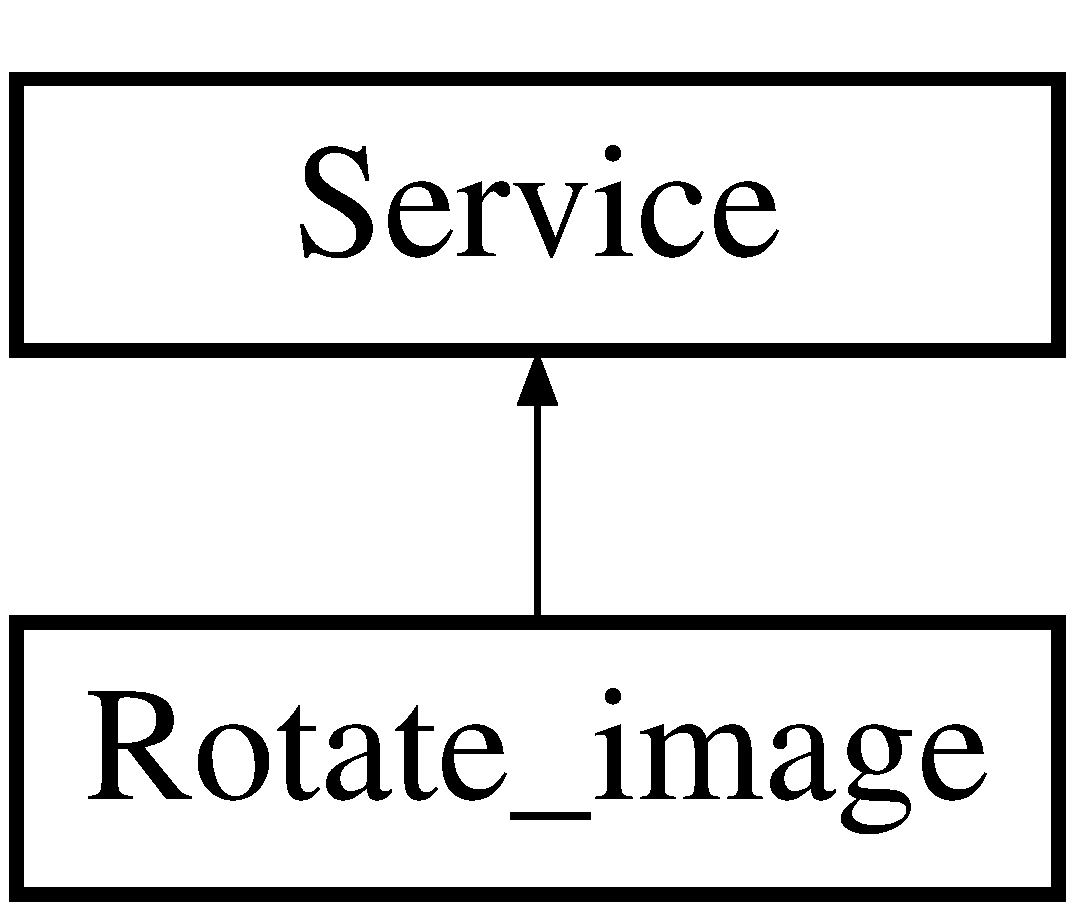
\includegraphics[height=2.000000cm]{class_rotate__image}
\end{center}
\end{figure}
\subsection*{Membri pubblici}
\begin{DoxyCompactItemize}
\item 
\hyperlink{class_rotate__image_a3bc89728401a10db11d79ea841f5c1e3}{Rotate\-\_\-image} ()
\begin{DoxyCompactList}\small\item\em Costruttore di default della classe \hyperlink{class_rotate__image}{Rotate\-\_\-image}. \end{DoxyCompactList}\item 
\hyperlink{class_rotate__image_a429fab26a1695b3b904a3f20eca28784}{Rotate\-\_\-image} (string name, string address, string port)
\begin{DoxyCompactList}\small\item\em Costruttore che inizializza l'istanza della classe \hyperlink{class_rotate__image}{Rotate\-\_\-image} con i parametri forniti. \end{DoxyCompactList}\item 
\hyperlink{class_rotate__image_a087945bc368560697a8dcb3728d045b7}{Rotate\-\_\-image} (string name, string address, string port, string \hyperlink{class_rotate__image_a30a932131de7296fef03f8c47d65594e}{path})
\begin{DoxyCompactList}\small\item\em Costruttore che inizializza l'istanza della classe \hyperlink{class_rotate__image}{Rotate\-\_\-image} con i parametri forniti. \end{DoxyCompactList}\item 
\hyperlink{class_rotate__image_a04bc5f8be9d04ddde1268ec7a8c086d7}{Rotate\-\_\-image} (\hyperlink{struct_service__description}{Service\-\_\-description} $\ast$\hyperlink{class_service_a55e991ff18c0dceca202388a771283dc}{s\-\_\-description})
\begin{DoxyCompactList}\small\item\em Costruttore che inizializza la classe \hyperlink{class_rotate__image}{Rotate\-\_\-image} con le informazioni ottenute dalla descrizione del servizio. \end{DoxyCompactList}\item 
\hyperlink{class_rotate__image_afbc9a78fd11c1181a516f31fa2341d8b}{Rotate\-\_\-image} (\hyperlink{struct_service__description}{Service\-\_\-description} $\ast$\hyperlink{class_service_a55e991ff18c0dceca202388a771283dc}{s\-\_\-description}, string \hyperlink{class_rotate__image_a30a932131de7296fef03f8c47d65594e}{path})
\begin{DoxyCompactList}\small\item\em Costruttore che inizializza la classe \hyperlink{class_rotate__image}{Rotate\-\_\-image} con le informazioni ottenute dalla descrizione del servizio e imposta la directory di lavoro con il path fornito in ingresso. \end{DoxyCompactList}\item 
\hypertarget{class_rotate__image_a81aa40308590dff5f6df897bc96329f4}{virtual \hyperlink{class_rotate__image_a81aa40308590dff5f6df897bc96329f4}{$\sim$\-Rotate\-\_\-image} ()}\label{class_rotate__image_a81aa40308590dff5f6df897bc96329f4}

\begin{DoxyCompactList}\small\item\em Distruttore della classe \hyperlink{class_rotate__image}{Rotate\-\_\-image}. \end{DoxyCompactList}\item 
bool \hyperlink{class_rotate__image_a58d6614345b8c9a70c7b052be314b5d7}{execute} ()
\begin{DoxyCompactList}\small\item\em Funzione che espleta il servizio di rotazione dell'immagine. \end{DoxyCompactList}\end{DoxyCompactItemize}
\subsection*{Membri privati}
\begin{DoxyCompactItemize}
\item 
void \hyperlink{class_rotate__image_a347de309e790cea7c72b5ff47c1591ce}{inizialize\-\_\-parameters} (string \hyperlink{class_rotate__image_a30a932131de7296fef03f8c47d65594e}{path})
\begin{DoxyCompactList}\small\item\em Inizializza l'istanza della classe \hyperlink{class_rotate__image}{Rotate\-\_\-image} (è chiamata da ogni costruttore). \end{DoxyCompactList}\end{DoxyCompactItemize}
\subsection*{Attributi privati}
\begin{DoxyCompactItemize}
\item 
\hypertarget{class_rotate__image_a30a932131de7296fef03f8c47d65594e}{string \hyperlink{class_rotate__image_a30a932131de7296fef03f8c47d65594e}{path}}\label{class_rotate__image_a30a932131de7296fef03f8c47d65594e}

\begin{DoxyCompactList}\small\item\em Directory di lavoro dove salvare i risultati temporanei (immagini sorgente e risultato della rotazione). \end{DoxyCompactList}\end{DoxyCompactItemize}
\subsection*{Altri membri ereditati}


\subsection{Descrizione dettagliata}
Classe che fornisce il servizio di rotazione di un immagine. E' una classe derivate di {\ttfamily \hyperlink{class_service}{Service}}. 

Definizione alla linea 114 del file Rotate\-\_\-image.\-h.



\subsection{Documentazione dei costruttori e dei distruttori}
\hypertarget{class_rotate__image_a3bc89728401a10db11d79ea841f5c1e3}{\index{Rotate\-\_\-image@{Rotate\-\_\-image}!Rotate\-\_\-image@{Rotate\-\_\-image}}
\index{Rotate\-\_\-image@{Rotate\-\_\-image}!Rotate_image@{Rotate\-\_\-image}}
\subsubsection[{Rotate\-\_\-image}]{\setlength{\rightskip}{0pt plus 5cm}Rotate\-\_\-image\-::\-Rotate\-\_\-image (
\begin{DoxyParamCaption}
{}
\end{DoxyParamCaption}
)}}\label{class_rotate__image_a3bc89728401a10db11d79ea841f5c1e3}


Costruttore di default della classe \hyperlink{class_rotate__image}{Rotate\-\_\-image}. 

Costruttore di default della classe \hyperlink{class_rotate__image}{Rotate\-\_\-image}. Provoca l'inizializzazione dei parametri di ingresso e uscita del servizio e setta la directory di lavoro sulla directory default. 

Definizione alla linea 5 del file Rotate\-\_\-image.\-cpp.

\hypertarget{class_rotate__image_a429fab26a1695b3b904a3f20eca28784}{\index{Rotate\-\_\-image@{Rotate\-\_\-image}!Rotate\-\_\-image@{Rotate\-\_\-image}}
\index{Rotate\-\_\-image@{Rotate\-\_\-image}!Rotate_image@{Rotate\-\_\-image}}
\subsubsection[{Rotate\-\_\-image}]{\setlength{\rightskip}{0pt plus 5cm}Rotate\-\_\-image\-::\-Rotate\-\_\-image (
\begin{DoxyParamCaption}
\item[{string}]{name, }
\item[{string}]{address, }
\item[{string}]{port}
\end{DoxyParamCaption}
)}}\label{class_rotate__image_a429fab26a1695b3b904a3f20eca28784}


Costruttore che inizializza l'istanza della classe \hyperlink{class_rotate__image}{Rotate\-\_\-image} con i parametri forniti. 


\begin{DoxyParams}[1]{Parametri}
\mbox{\tt in}  & {\em name} & Nome da assegnare al servizio. \\
\hline
\mbox{\tt in}  & {\em address} & Indirizzo I\-P del service provider che fornisce il servizio. \\
\hline
\mbox{\tt in}  & {\em port} & Porta di ascolto del service provider che fornisce il servizio. Costruttore che inizializza l'istanza della classe \hyperlink{class_rotate__image}{Rotate\-\_\-image} con nome, indirizzo e porta forniti in ingresso, inizializza i parametri di ingresso e uscita del servizio e setta la directory di lavoro sulla directory default. \\
\hline
\end{DoxyParams}


Definizione alla linea 9 del file Rotate\-\_\-image.\-cpp.

\hypertarget{class_rotate__image_a087945bc368560697a8dcb3728d045b7}{\index{Rotate\-\_\-image@{Rotate\-\_\-image}!Rotate\-\_\-image@{Rotate\-\_\-image}}
\index{Rotate\-\_\-image@{Rotate\-\_\-image}!Rotate_image@{Rotate\-\_\-image}}
\subsubsection[{Rotate\-\_\-image}]{\setlength{\rightskip}{0pt plus 5cm}Rotate\-\_\-image\-::\-Rotate\-\_\-image (
\begin{DoxyParamCaption}
\item[{string}]{name, }
\item[{string}]{address, }
\item[{string}]{port, }
\item[{string}]{path}
\end{DoxyParamCaption}
)}}\label{class_rotate__image_a087945bc368560697a8dcb3728d045b7}


Costruttore che inizializza l'istanza della classe \hyperlink{class_rotate__image}{Rotate\-\_\-image} con i parametri forniti. 


\begin{DoxyParams}[1]{Parametri}
\mbox{\tt in}  & {\em name} & Nome da assegnare al servizio. \\
\hline
\mbox{\tt in}  & {\em address} & Indirizzo I\-P del service provider che fornisce il servizio. \\
\hline
\mbox{\tt in}  & {\em port} & Porta di ascolto del service provider che fornisce il servizio. \\
\hline
\mbox{\tt in}  & {\em path} & Directory di lavoro da assegnare al servizio dove salvare i files temporanei. Costruttore che inizializza l'istanza della classe \hyperlink{class_rotate__image}{Rotate\-\_\-image} con nome, indirizzo e porta forniti in ingresso, inizializza i parametri di ingresso e uscita del servizio e imposta la directory di lavoro con il path fornito in ingresso. \\
\hline
\end{DoxyParams}


Definizione alla linea 12 del file Rotate\-\_\-image.\-cpp.

\hypertarget{class_rotate__image_a04bc5f8be9d04ddde1268ec7a8c086d7}{\index{Rotate\-\_\-image@{Rotate\-\_\-image}!Rotate\-\_\-image@{Rotate\-\_\-image}}
\index{Rotate\-\_\-image@{Rotate\-\_\-image}!Rotate_image@{Rotate\-\_\-image}}
\subsubsection[{Rotate\-\_\-image}]{\setlength{\rightskip}{0pt plus 5cm}Rotate\-\_\-image\-::\-Rotate\-\_\-image (
\begin{DoxyParamCaption}
\item[{{\bf Service\-\_\-description} $\ast$}]{s\-\_\-description}
\end{DoxyParamCaption}
)}}\label{class_rotate__image_a04bc5f8be9d04ddde1268ec7a8c086d7}


Costruttore che inizializza la classe \hyperlink{class_rotate__image}{Rotate\-\_\-image} con le informazioni ottenute dalla descrizione del servizio. 


\begin{DoxyParams}[1]{Parametri}
\mbox{\tt in}  & {\em s\-\_\-description} & Descrizione del servizio. \\
\hline
\end{DoxyParams}


Definizione alla linea 15 del file Rotate\-\_\-image.\-cpp.

\hypertarget{class_rotate__image_afbc9a78fd11c1181a516f31fa2341d8b}{\index{Rotate\-\_\-image@{Rotate\-\_\-image}!Rotate\-\_\-image@{Rotate\-\_\-image}}
\index{Rotate\-\_\-image@{Rotate\-\_\-image}!Rotate_image@{Rotate\-\_\-image}}
\subsubsection[{Rotate\-\_\-image}]{\setlength{\rightskip}{0pt plus 5cm}Rotate\-\_\-image\-::\-Rotate\-\_\-image (
\begin{DoxyParamCaption}
\item[{{\bf Service\-\_\-description} $\ast$}]{s\-\_\-description, }
\item[{string}]{path}
\end{DoxyParamCaption}
)}}\label{class_rotate__image_afbc9a78fd11c1181a516f31fa2341d8b}


Costruttore che inizializza la classe \hyperlink{class_rotate__image}{Rotate\-\_\-image} con le informazioni ottenute dalla descrizione del servizio e imposta la directory di lavoro con il path fornito in ingresso. 


\begin{DoxyParams}[1]{Parametri}
\mbox{\tt in}  & {\em s\-\_\-description} & Descrizione del servizio. \\
\hline
\mbox{\tt in}  & {\em path} & Directory di lavoro da assegnare al servizio dove salvare i files temporanei. \\
\hline
\end{DoxyParams}


Definizione alla linea 21 del file Rotate\-\_\-image.\-cpp.



\subsection{Documentazione delle funzioni membro}
\hypertarget{class_rotate__image_a58d6614345b8c9a70c7b052be314b5d7}{\index{Rotate\-\_\-image@{Rotate\-\_\-image}!execute@{execute}}
\index{execute@{execute}!Rotate_image@{Rotate\-\_\-image}}
\subsubsection[{execute}]{\setlength{\rightskip}{0pt plus 5cm}bool Rotate\-\_\-image\-::execute (
\begin{DoxyParamCaption}
{}
\end{DoxyParamCaption}
)\hspace{0.3cm}{\ttfamily [virtual]}}}\label{class_rotate__image_a58d6614345b8c9a70c7b052be314b5d7}


Funzione che espleta il servizio di rotazione dell'immagine. 

\begin{DoxyReturn}{Restituisce}
Risultato dell'esecuzione, {\ttfamily true} in caso di successo e {\ttfamily false} altrimenti. Il servizio di rotazione viene effettuato come segue\-: \begin{DoxyItemize}
\item genera nella directory di lavoro l'immagine da elaborare a partire dal parametro {\ttfamily buffer} in ingresso al servizio \item vi applica l'operatore di rotazione ottenendo una nuova immagine (da ritornare al chiamante) \item compila il parametro di uscita del servizio (di tipo {\itshape buffer}) con i dati dell'immagine ruotata \item se {\itshape R\-E\-M\-O\-V\-E\-\_\-\-I\-M\-A\-G\-E\-S} è impostato a {\ttfamily true}, rimuove le due immagini appena create (ormai inutili) dalla directory di lavoro \end{DoxyItemize}

\end{DoxyReturn}


Reimplementa \hyperlink{class_service}{Service}.



Definizione alla linea 40 del file Rotate\-\_\-image.\-cpp.

\hypertarget{class_rotate__image_a347de309e790cea7c72b5ff47c1591ce}{\index{Rotate\-\_\-image@{Rotate\-\_\-image}!inizialize\-\_\-parameters@{inizialize\-\_\-parameters}}
\index{inizialize\-\_\-parameters@{inizialize\-\_\-parameters}!Rotate_image@{Rotate\-\_\-image}}
\subsubsection[{inizialize\-\_\-parameters}]{\setlength{\rightskip}{0pt plus 5cm}Rotate\-\_\-image\-::inizialize\-\_\-parameters (
\begin{DoxyParamCaption}
\item[{string}]{path}
\end{DoxyParamCaption}
)\hspace{0.3cm}{\ttfamily [private]}}}\label{class_rotate__image_a347de309e790cea7c72b5ff47c1591ce}


Inizializza l'istanza della classe \hyperlink{class_rotate__image}{Rotate\-\_\-image} (è chiamata da ogni costruttore). 


\begin{DoxyParams}[1]{Parametri}
\mbox{\tt in}  & {\em path} & Directory di lavoro da assegnare al servizio dove salvare i files temporanei. Inizializza l'istanza della classe \hyperlink{class_rotate__image}{Rotate\-\_\-image} come segue\-: \begin{DoxyItemize}
\item genera un parametro in ingresso di tipo {\ttfamily buffer} atto a mantenere le informazioni relative all'immagine da elaborare \item genera un parametro in ingresso di tipo {\ttfamily integer} che conterrà l'informazione di rotazione dell'immagine (di quanti gradi ruotare l'immagine) \item genera un parametro in uscita di tipo {\itshape buffer} per l'immagine ruotata \item crea la directory di lavoro del servizio se questa non esiste \end{DoxyItemize}
\\
\hline
\end{DoxyParams}


Definizione alla linea 30 del file Rotate\-\_\-image.\-cpp.



La documentazione per questa classe è stata generata a partire dai seguenti file\-:\begin{DoxyCompactItemize}
\item 
C\-:/\-Users/\-Matteo/\-Dropbox/\-Universita/\-Sistemi Operativi e Programmazione Distribuita/\-Progetto/\-Service\-\_\-\-Oriented\-\_\-\-Architecture/\-Sources/\-Application/\-Image\-\_\-manipulation\-\_\-server/\hyperlink{_rotate__image_8h}{Rotate\-\_\-image.\-h}\item 
C\-:/\-Users/\-Matteo/\-Dropbox/\-Universita/\-Sistemi Operativi e Programmazione Distribuita/\-Progetto/\-Service\-\_\-\-Oriented\-\_\-\-Architecture/\-Sources/\-Application/\-Image\-\_\-manipulation\-\_\-server/Rotate\-\_\-image.\-cpp\end{DoxyCompactItemize}

\hypertarget{class_service}{\section{Riferimenti per la classe Service}
\label{class_service}\index{Service@{Service}}
}


Classe che contiene la descrizione del servizio, l'elenco dei parametri di ingresso e un'istanza della classe {\ttfamily \hyperlink{class_responce}{Responce}}.  




{\ttfamily \#include $<$Service.\-h$>$}

Diagramma delle classi per Service\begin{figure}[H]
\begin{center}
\leavevmode
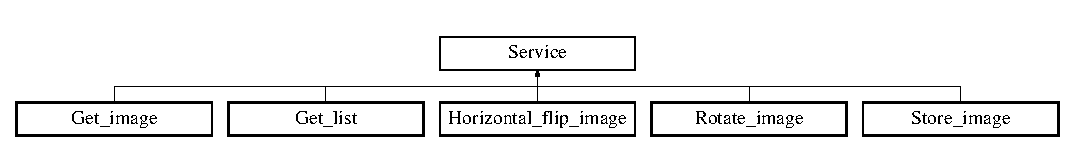
\includegraphics[height=1.588652cm]{class_service}
\end{center}
\end{figure}
\subsection*{Membri pubblici}
\begin{DoxyCompactItemize}
\item 
\hypertarget{class_service_acc246c9f7ed3c51e2d91d10fe257513f}{\hyperlink{class_service_acc246c9f7ed3c51e2d91d10fe257513f}{Service} ()}\label{class_service_acc246c9f7ed3c51e2d91d10fe257513f}

\begin{DoxyCompactList}\small\item\em Costruttore di default della classe \hyperlink{class_service}{Service}. \end{DoxyCompactList}\item 
\hyperlink{class_service_aaf16ba3725a4a48487650ed907999bfc}{Service} (string name, string address, string port)
\begin{DoxyCompactList}\small\item\em Costruttore che inizializza la classe \hyperlink{class_service}{Service} con i parametri forniti. \end{DoxyCompactList}\item 
\hyperlink{class_service_ad838a974b007483f2c43cf66b578fccc}{Service} (\hyperlink{struct_service__description}{Service\-\_\-description} $\ast$\hyperlink{class_service_a55e991ff18c0dceca202388a771283dc}{s\-\_\-description})
\begin{DoxyCompactList}\small\item\em Costruttore che inizializza la classe \hyperlink{class_service}{Service} con le informazioni ottenute dalla descrizione del servizio. \end{DoxyCompactList}\item 
\hypertarget{class_service_af6c3577b59652ac817d1d76aaccee904}{virtual \hyperlink{class_service_af6c3577b59652ac817d1d76aaccee904}{$\sim$\-Service} ()}\label{class_service_af6c3577b59652ac817d1d76aaccee904}

\begin{DoxyCompactList}\small\item\em Distruttore della classe \hyperlink{class_service}{Service}. \end{DoxyCompactList}\item 
void \hyperlink{class_service_a3905da32f595397967e7aada8300ec6c}{add\-\_\-parameter} (\hyperlink{_types_8h_a224b9163917ac32fc95a60d8c1eec3aa}{Direction} direction, \hyperlink{_types_8h_a1d1cfd8ffb84e947f82999c682b666a7}{Type} type)
\begin{DoxyCompactList}\small\item\em Aggiunge un parametro di tipo {\itshape type} alla lista dei parametri (di ingresso o uscita) del servizio. \end{DoxyCompactList}\item 
bool \hyperlink{class_service_ab475411bca62ebf3cbbcf338285f4975}{set\-\_\-input\-\_\-parameters} (vector$<$ \hyperlink{struct_parameter}{Parameter} $>$ \hyperlink{class_service_a92a0bf45e91da701d22152651d3c7907}{parameters})
\begin{DoxyCompactList}\small\item\em Setta i parametri di ingresso del servizio con il valore dei parametri forniti. \end{DoxyCompactList}\item 
void \hyperlink{class_service_a091d68c0751de158de2c2f64aeb9cdc8}{set\-\_\-name} (string name)
\begin{DoxyCompactList}\small\item\em Setta il nome del servizio con il valore passato come parametro. \end{DoxyCompactList}\item 
void \hyperlink{class_service_a69f551db5d32632d9558df9de84f023c}{set\-\_\-port} (string port)
\begin{DoxyCompactList}\small\item\em Setta la porta associata al servizio con il valore passato come parametro. \end{DoxyCompactList}\item 
void \hyperlink{class_service_abee2b18fa2bb31c31915c2cda525355b}{set\-\_\-address} (string address)
\begin{DoxyCompactList}\small\item\em Setta l'indirizzo associato al servizio con il valore passato come parametro. \end{DoxyCompactList}\item 
string \hyperlink{class_service_af7450cf76dd2c06d556b55c8555670f5}{get\-\_\-name} ()
\begin{DoxyCompactList}\small\item\em Ritorna al chiamante il nome del servizio. \end{DoxyCompactList}\item 
string \hyperlink{class_service_acc2d27605b7e2e45d28c6c18c117ee48}{get\-\_\-port} ()
\begin{DoxyCompactList}\small\item\em Ritorna al chiamante la porta associata al servizio. \end{DoxyCompactList}\item 
string \hyperlink{class_service_a4255bff226f0c507ed997d8474426cff}{get\-\_\-address} ()
\begin{DoxyCompactList}\small\item\em Ritorna al chiamante l'indirizzo associato al servizio. \end{DoxyCompactList}\item 
\hyperlink{struct_service__description}{Service\-\_\-description} $\ast$ \hyperlink{class_service_aa3b79916f4e6f1be8e8189fc1a6b02ad}{get\-\_\-description} ()
\begin{DoxyCompactList}\small\item\em Ritorna al chiamante la descrizione completa del servizio. \end{DoxyCompactList}\item 
bool \hyperlink{class_service_a4952a5f82a2c49a83fe5548c3865458b}{send\-\_\-service\-\_\-request} (int $\ast$socket)
\begin{DoxyCompactList}\small\item\em Invia sul {\itshape Socket} la richiesta di servizio al service provider che lo fornisce. \end{DoxyCompactList}\item 
bool \hyperlink{class_service_a67f01dff03c913cd0ba77cf073e829fd}{receive\-\_\-service\-\_\-request} (int socket)
\begin{DoxyCompactList}\small\item\em Riceve sul {\itshape Socket} la richiesta di servizio da parte del {\itshape Client}. \end{DoxyCompactList}\item 
bool \hyperlink{class_service_a4efee47181b839b6e03146a439f924db}{send\-\_\-service\-\_\-responce} (int socket)
\begin{DoxyCompactList}\small\item\em Invia sul {\itshape Socket} i parametri di risposta di un servizio chiamando l'omonimo servizio della classe {\ttfamily \hyperlink{class_responce}{Responce}}. \end{DoxyCompactList}\item 
bool \hyperlink{class_service_a3e86a7b9b19d5ff72c952f980b61e3d8}{receive\-\_\-service\-\_\-responce} (int socket)
\begin{DoxyCompactList}\small\item\em Riceve sul {\itshape Socket} i parametri di risposta di un servizio chiamando l'omonimo servizio della classe {\ttfamily \hyperlink{class_responce}{Responce}}. \end{DoxyCompactList}\item 
virtual bool \hyperlink{class_service_a4aed56f17af847cab41a911c1555ac2a}{responce\-\_\-decode} (string folder\-\_\-path)
\begin{DoxyCompactList}\small\item\em Crea un file al path specificato a partire dal parametro di risposta del servizio. \end{DoxyCompactList}\item 
virtual bool \hyperlink{class_service_af6bbad3f7fa3d4ee685a97f8022752e5}{responce\-\_\-decode} (vector$<$ string $>$ $\ast$file\-\_\-list)
\begin{DoxyCompactList}\small\item\em Crea la lista dei file presenti sul server di storage (in forma vettoriale) a partire dal parametro di risposta del servizio (tipo stringa). \end{DoxyCompactList}\item 
\hypertarget{class_service_aef1e4cf743a29f48b3708915f2bb2f37}{virtual bool {\bfseries execute} ()}\label{class_service_aef1e4cf743a29f48b3708915f2bb2f37}

\end{DoxyCompactItemize}
\subsection*{Attributi protetti}
\begin{DoxyCompactItemize}
\item 
\hypertarget{class_service_a55e991ff18c0dceca202388a771283dc}{\hyperlink{struct_service__description}{Service\-\_\-description} \hyperlink{class_service_a55e991ff18c0dceca202388a771283dc}{s\-\_\-description}}\label{class_service_a55e991ff18c0dceca202388a771283dc}

\begin{DoxyCompactList}\small\item\em Descrizione del servizio. \end{DoxyCompactList}\item 
\hypertarget{class_service_a92a0bf45e91da701d22152651d3c7907}{vector$<$ \hyperlink{struct_parameter}{Parameter} $>$ \hyperlink{class_service_a92a0bf45e91da701d22152651d3c7907}{parameters}}\label{class_service_a92a0bf45e91da701d22152651d3c7907}

\begin{DoxyCompactList}\small\item\em Vettore di tipo {\ttfamily \hyperlink{struct_parameter}{Parameter}} che contiene i parametri di ingresso del servizio. \end{DoxyCompactList}\item 
\hypertarget{class_service_af32489d66225d9cc691e68d1af386e9e}{\hyperlink{class_responce}{Responce} \hyperlink{class_service_af32489d66225d9cc691e68d1af386e9e}{responce}}\label{class_service_af32489d66225d9cc691e68d1af386e9e}

\begin{DoxyCompactList}\small\item\em Istanza della classe {\itshape \hyperlink{class_responce}{Responce}} associata al servizio. \end{DoxyCompactList}\end{DoxyCompactItemize}


\subsection{Descrizione dettagliata}
Classe che contiene la descrizione del servizio, l'elenco dei parametri di ingresso e un'istanza della classe {\ttfamily \hyperlink{class_responce}{Responce}}. 

Definizione alla linea 165 del file Service.\-h.



\subsection{Documentazione dei costruttori e dei distruttori}
\hypertarget{class_service_aaf16ba3725a4a48487650ed907999bfc}{\index{Service@{Service}!Service@{Service}}
\index{Service@{Service}!Service@{Service}}
\subsubsection[{Service}]{\setlength{\rightskip}{0pt plus 5cm}Service\-::\-Service (
\begin{DoxyParamCaption}
\item[{string}]{name, }
\item[{string}]{address, }
\item[{string}]{port}
\end{DoxyParamCaption}
)}}\label{class_service_aaf16ba3725a4a48487650ed907999bfc}


Costruttore che inizializza la classe \hyperlink{class_service}{Service} con i parametri forniti. 


\begin{DoxyParams}[1]{Parametri}
\mbox{\tt in}  & {\em name} & Nome del servizio. \\
\hline
\mbox{\tt in}  & {\em address} & Indirizzo I\-P del service provider che fornisce il servizio. \\
\hline
\mbox{\tt in}  & {\em port} & Porta di ascolto del service provider che fornisce il servizio. \\
\hline
\end{DoxyParams}


Definizione alla linea 5 del file Service.\-cpp.

\hypertarget{class_service_ad838a974b007483f2c43cf66b578fccc}{\index{Service@{Service}!Service@{Service}}
\index{Service@{Service}!Service@{Service}}
\subsubsection[{Service}]{\setlength{\rightskip}{0pt plus 5cm}Service\-::\-Service (
\begin{DoxyParamCaption}
\item[{{\bf Service\-\_\-description} $\ast$}]{s\-\_\-description}
\end{DoxyParamCaption}
)}}\label{class_service_ad838a974b007483f2c43cf66b578fccc}


Costruttore che inizializza la classe \hyperlink{class_service}{Service} con le informazioni ottenute dalla descrizione del servizio. 


\begin{DoxyParams}[1]{Parametri}
\mbox{\tt in}  & {\em s\-\_\-description} & Descrizione del servizio. \\
\hline
\end{DoxyParams}


Definizione alla linea 11 del file Service.\-cpp.



\subsection{Documentazione delle funzioni membro}
\hypertarget{class_service_a3905da32f595397967e7aada8300ec6c}{\index{Service@{Service}!add\-\_\-parameter@{add\-\_\-parameter}}
\index{add\-\_\-parameter@{add\-\_\-parameter}!Service@{Service}}
\subsubsection[{add\-\_\-parameter}]{\setlength{\rightskip}{0pt plus 5cm}void Service\-::add\-\_\-parameter (
\begin{DoxyParamCaption}
\item[{{\bf Direction}}]{direction, }
\item[{{\bf Type}}]{type}
\end{DoxyParamCaption}
)}}\label{class_service_a3905da32f595397967e7aada8300ec6c}


Aggiunge un parametro di tipo {\itshape type} alla lista dei parametri (di ingresso o uscita) del servizio. 


\begin{DoxyParams}[1]{Parametri}
\mbox{\tt in}  & {\em direction} & Direzione del parametro da aggiungere al servizio. \\
\hline
\mbox{\tt in}  & {\em type} & Tipo del parametro da aggiungere al servizio. \\
\hline
\end{DoxyParams}


Definizione alla linea 28 del file Service.\-cpp.

\hypertarget{class_service_a4255bff226f0c507ed997d8474426cff}{\index{Service@{Service}!get\-\_\-address@{get\-\_\-address}}
\index{get\-\_\-address@{get\-\_\-address}!Service@{Service}}
\subsubsection[{get\-\_\-address}]{\setlength{\rightskip}{0pt plus 5cm}string Service\-::get\-\_\-address (
\begin{DoxyParamCaption}
{}
\end{DoxyParamCaption}
)}}\label{class_service_a4255bff226f0c507ed997d8474426cff}


Ritorna al chiamante l'indirizzo associato al servizio. 

\begin{DoxyReturn}{Restituisce}
Indirizzo del service provider che fornisce il servizio. 
\end{DoxyReturn}


Definizione alla linea 79 del file Service.\-cpp.

\hypertarget{class_service_aa3b79916f4e6f1be8e8189fc1a6b02ad}{\index{Service@{Service}!get\-\_\-description@{get\-\_\-description}}
\index{get\-\_\-description@{get\-\_\-description}!Service@{Service}}
\subsubsection[{get\-\_\-description}]{\setlength{\rightskip}{0pt plus 5cm}{\bf Service\-\_\-description} $\ast$ Service\-::get\-\_\-description (
\begin{DoxyParamCaption}
{}
\end{DoxyParamCaption}
)}}\label{class_service_aa3b79916f4e6f1be8e8189fc1a6b02ad}


Ritorna al chiamante la descrizione completa del servizio. 

\begin{DoxyReturn}{Restituisce}
Descrizione completa del servizio. 
\end{DoxyReturn}


Definizione alla linea 83 del file Service.\-cpp.

\hypertarget{class_service_af7450cf76dd2c06d556b55c8555670f5}{\index{Service@{Service}!get\-\_\-name@{get\-\_\-name}}
\index{get\-\_\-name@{get\-\_\-name}!Service@{Service}}
\subsubsection[{get\-\_\-name}]{\setlength{\rightskip}{0pt plus 5cm}string Service\-::get\-\_\-name (
\begin{DoxyParamCaption}
{}
\end{DoxyParamCaption}
)}}\label{class_service_af7450cf76dd2c06d556b55c8555670f5}


Ritorna al chiamante il nome del servizio. 

\begin{DoxyReturn}{Restituisce}
Nome del servizio. 
\end{DoxyReturn}


Definizione alla linea 71 del file Service.\-cpp.

\hypertarget{class_service_acc2d27605b7e2e45d28c6c18c117ee48}{\index{Service@{Service}!get\-\_\-port@{get\-\_\-port}}
\index{get\-\_\-port@{get\-\_\-port}!Service@{Service}}
\subsubsection[{get\-\_\-port}]{\setlength{\rightskip}{0pt plus 5cm}string Service\-::get\-\_\-port (
\begin{DoxyParamCaption}
{}
\end{DoxyParamCaption}
)}}\label{class_service_acc2d27605b7e2e45d28c6c18c117ee48}


Ritorna al chiamante la porta associata al servizio. 

\begin{DoxyReturn}{Restituisce}
Porta di ascolto del service provider che fornisce il servizio. 
\end{DoxyReturn}


Definizione alla linea 75 del file Service.\-cpp.

\hypertarget{class_service_a67f01dff03c913cd0ba77cf073e829fd}{\index{Service@{Service}!receive\-\_\-service\-\_\-request@{receive\-\_\-service\-\_\-request}}
\index{receive\-\_\-service\-\_\-request@{receive\-\_\-service\-\_\-request}!Service@{Service}}
\subsubsection[{receive\-\_\-service\-\_\-request}]{\setlength{\rightskip}{0pt plus 5cm}bool Service\-::receive\-\_\-service\-\_\-request (
\begin{DoxyParamCaption}
\item[{int}]{socket}
\end{DoxyParamCaption}
)}}\label{class_service_a67f01dff03c913cd0ba77cf073e829fd}


Riceve sul {\itshape Socket} la richiesta di servizio da parte del {\itshape Client}. 


\begin{DoxyParams}[1]{Parametri}
\mbox{\tt in}  & {\em socket} & {\itshape Socket} sul quale ricevere la richiesta di servizio. \\
\hline
\end{DoxyParams}
\begin{DoxyReturn}{Restituisce}
Risultato della ricezione della richiesta, {\ttfamily true} in caso di successo e {\ttfamily false} altrimenti. La ricezione delle richiesta di servizio avviene nel seguente modo\-: \begin{DoxyItemize}
\item riceve il nome del servizio richiesto e rifiuta la richiesta se il servizio non viene riconosciuto dal service provider \item riceve il numero di parametri del servizio richiesto e rifiuta la richiesta se il numero non coincide con quello atteso \item per ogni parametro riceve il tipo e rifiuta la richiesta se il tipo non coincide con quello atteso \item per ogni parametro riceve il valore effettivo del parametro \end{DoxyItemize}

\end{DoxyReturn}


Definizione alla linea 122 del file Service.\-cpp.

\hypertarget{class_service_a3e86a7b9b19d5ff72c952f980b61e3d8}{\index{Service@{Service}!receive\-\_\-service\-\_\-responce@{receive\-\_\-service\-\_\-responce}}
\index{receive\-\_\-service\-\_\-responce@{receive\-\_\-service\-\_\-responce}!Service@{Service}}
\subsubsection[{receive\-\_\-service\-\_\-responce}]{\setlength{\rightskip}{0pt plus 5cm}bool Service\-::receive\-\_\-service\-\_\-responce (
\begin{DoxyParamCaption}
\item[{int}]{socket}
\end{DoxyParamCaption}
)}}\label{class_service_a3e86a7b9b19d5ff72c952f980b61e3d8}


Riceve sul {\itshape Socket} i parametri di risposta di un servizio chiamando l'omonimo servizio della classe {\ttfamily \hyperlink{class_responce}{Responce}}. 


\begin{DoxyParams}[1]{Parametri}
\mbox{\tt in}  & {\em socket} & {\itshape Socket} sul quale ricevere i parametri di risposta del servizio. \\
\hline
\end{DoxyParams}
\begin{DoxyReturn}{Restituisce}
Risultato della ricezione della risposta, {\ttfamily true} in caso di successo e {\ttfamily false} altrimenti. 
\end{DoxyReturn}


Definizione alla linea 150 del file Service.\-cpp.

\hypertarget{class_service_a4aed56f17af847cab41a911c1555ac2a}{\index{Service@{Service}!responce\-\_\-decode@{responce\-\_\-decode}}
\index{responce\-\_\-decode@{responce\-\_\-decode}!Service@{Service}}
\subsubsection[{responce\-\_\-decode}]{\setlength{\rightskip}{0pt plus 5cm}bool Service\-::responce\-\_\-decode (
\begin{DoxyParamCaption}
\item[{string}]{image\-\_\-path}
\end{DoxyParamCaption}
)\hspace{0.3cm}{\ttfamily [virtual]}}}\label{class_service_a4aed56f17af847cab41a911c1555ac2a}


Crea un file al path specificato a partire dal parametro di risposta del servizio. 


\begin{DoxyParams}[1]{Parametri}
\mbox{\tt in}  & {\em image\-\_\-path} & Path relativo all'immagine da realizzare (comprensivo di nome ed estensione del file). \\
\hline
\end{DoxyParams}
\begin{DoxyReturn}{Restituisce}
Risultato della creazione del file, {\ttfamily true} in caso di successo e {\ttfamily false} altrimenti. 
\end{DoxyReturn}


Definizione alla linea 155 del file Service.\-cpp.

\hypertarget{class_service_af6bbad3f7fa3d4ee685a97f8022752e5}{\index{Service@{Service}!responce\-\_\-decode@{responce\-\_\-decode}}
\index{responce\-\_\-decode@{responce\-\_\-decode}!Service@{Service}}
\subsubsection[{responce\-\_\-decode}]{\setlength{\rightskip}{0pt plus 5cm}bool Service\-::responce\-\_\-decode (
\begin{DoxyParamCaption}
\item[{vector$<$ string $>$ $\ast$}]{file\-\_\-list}
\end{DoxyParamCaption}
)\hspace{0.3cm}{\ttfamily [virtual]}}}\label{class_service_af6bbad3f7fa3d4ee685a97f8022752e5}


Crea la lista dei file presenti sul server di storage (in forma vettoriale) a partire dal parametro di risposta del servizio (tipo stringa). 


\begin{DoxyParams}[1]{Parametri}
\mbox{\tt out}  & {\em file\-\_\-list} & Lista di file presenti sul server di storage di immagini. \\
\hline
\end{DoxyParams}
\begin{DoxyReturn}{Restituisce}
Risultato della ricezione della risposta, {\ttfamily true} in caso di successo e {\ttfamily false} altrimenti. 
\end{DoxyReturn}


Definizione alla linea 163 del file Service.\-cpp.

\hypertarget{class_service_a4952a5f82a2c49a83fe5548c3865458b}{\index{Service@{Service}!send\-\_\-service\-\_\-request@{send\-\_\-service\-\_\-request}}
\index{send\-\_\-service\-\_\-request@{send\-\_\-service\-\_\-request}!Service@{Service}}
\subsubsection[{send\-\_\-service\-\_\-request}]{\setlength{\rightskip}{0pt plus 5cm}bool Service\-::send\-\_\-service\-\_\-request (
\begin{DoxyParamCaption}
\item[{int $\ast$}]{socket}
\end{DoxyParamCaption}
)}}\label{class_service_a4952a5f82a2c49a83fe5548c3865458b}


Invia sul {\itshape Socket} la richiesta di servizio al service provider che lo fornisce. 


\begin{DoxyParams}[1]{Parametri}
\mbox{\tt out}  & {\em socket} & {\itshape Socket} sul quale inviare la richiesta di servizio. \\
\hline
\end{DoxyParams}
\begin{DoxyReturn}{Restituisce}
Risultato dell'invio della richiesta, {\ttfamily true} in caso di successo e {\ttfamily false} altrimenti. L'invio delle richiesta di servizio avviene nel seguente modo\-: \begin{DoxyItemize}
\item invia il nome del servizio e si pone in attesa dell'accettazione della richiesta \item invia il numero di parametri del servizio e si pone in attesa della conferma \item per ogni parametro invia il tipo e si pone in attesa della conferma \item per ogni parametro invia il valore effettivo del parametro \end{DoxyItemize}

\end{DoxyReturn}


Definizione alla linea 87 del file Service.\-cpp.

\hypertarget{class_service_a4efee47181b839b6e03146a439f924db}{\index{Service@{Service}!send\-\_\-service\-\_\-responce@{send\-\_\-service\-\_\-responce}}
\index{send\-\_\-service\-\_\-responce@{send\-\_\-service\-\_\-responce}!Service@{Service}}
\subsubsection[{send\-\_\-service\-\_\-responce}]{\setlength{\rightskip}{0pt plus 5cm}bool Service\-::send\-\_\-service\-\_\-responce (
\begin{DoxyParamCaption}
\item[{int}]{socket}
\end{DoxyParamCaption}
)}}\label{class_service_a4efee47181b839b6e03146a439f924db}


Invia sul {\itshape Socket} i parametri di risposta di un servizio chiamando l'omonimo servizio della classe {\ttfamily \hyperlink{class_responce}{Responce}}. 


\begin{DoxyParams}[1]{Parametri}
\mbox{\tt in}  & {\em socket} & {\itshape Socket} sul quale inviare i parametri di risposta del servizio. \\
\hline
\end{DoxyParams}
\begin{DoxyReturn}{Restituisce}
Risultato dell'invio della risposta, {\ttfamily true} in caso di successo e {\ttfamily false} altrimenti. 
\end{DoxyReturn}


Definizione alla linea 146 del file Service.\-cpp.

\hypertarget{class_service_abee2b18fa2bb31c31915c2cda525355b}{\index{Service@{Service}!set\-\_\-address@{set\-\_\-address}}
\index{set\-\_\-address@{set\-\_\-address}!Service@{Service}}
\subsubsection[{set\-\_\-address}]{\setlength{\rightskip}{0pt plus 5cm}void Service\-::set\-\_\-address (
\begin{DoxyParamCaption}
\item[{string}]{address}
\end{DoxyParamCaption}
)}}\label{class_service_abee2b18fa2bb31c31915c2cda525355b}


Setta l'indirizzo associato al servizio con il valore passato come parametro. 


\begin{DoxyParams}[1]{Parametri}
\mbox{\tt in}  & {\em address} & Indirizzo del service provider che fornisce il servizio. \\
\hline
\end{DoxyParams}


Definizione alla linea 67 del file Service.\-cpp.

\hypertarget{class_service_ab475411bca62ebf3cbbcf338285f4975}{\index{Service@{Service}!set\-\_\-input\-\_\-parameters@{set\-\_\-input\-\_\-parameters}}
\index{set\-\_\-input\-\_\-parameters@{set\-\_\-input\-\_\-parameters}!Service@{Service}}
\subsubsection[{set\-\_\-input\-\_\-parameters}]{\setlength{\rightskip}{0pt plus 5cm}bool Service\-::set\-\_\-input\-\_\-parameters (
\begin{DoxyParamCaption}
\item[{vector$<$ {\bf Parameter} $>$}]{parameters}
\end{DoxyParamCaption}
)}}\label{class_service_ab475411bca62ebf3cbbcf338285f4975}


Setta i parametri di ingresso del servizio con il valore dei parametri forniti. 


\begin{DoxyParams}[1]{Parametri}
\mbox{\tt in}  & {\em parameters} & Vettore di parametri con cui settare i parametri di ingresso del servizio. \\
\hline
\end{DoxyParams}
\begin{DoxyReturn}{Restituisce}
Risultato dell'esecuzione, {\ttfamily true} in caso di successo e {\ttfamily false} altrimenti. 
\end{DoxyReturn}


Definizione alla linea 42 del file Service.\-cpp.

\hypertarget{class_service_a091d68c0751de158de2c2f64aeb9cdc8}{\index{Service@{Service}!set\-\_\-name@{set\-\_\-name}}
\index{set\-\_\-name@{set\-\_\-name}!Service@{Service}}
\subsubsection[{set\-\_\-name}]{\setlength{\rightskip}{0pt plus 5cm}void Service\-::set\-\_\-name (
\begin{DoxyParamCaption}
\item[{string}]{name}
\end{DoxyParamCaption}
)}}\label{class_service_a091d68c0751de158de2c2f64aeb9cdc8}


Setta il nome del servizio con il valore passato come parametro. 


\begin{DoxyParams}[1]{Parametri}
\mbox{\tt in}  & {\em name} & Nome del servizio. \\
\hline
\end{DoxyParams}


Definizione alla linea 59 del file Service.\-cpp.

\hypertarget{class_service_a69f551db5d32632d9558df9de84f023c}{\index{Service@{Service}!set\-\_\-port@{set\-\_\-port}}
\index{set\-\_\-port@{set\-\_\-port}!Service@{Service}}
\subsubsection[{set\-\_\-port}]{\setlength{\rightskip}{0pt plus 5cm}void Service\-::set\-\_\-port (
\begin{DoxyParamCaption}
\item[{string}]{port}
\end{DoxyParamCaption}
)}}\label{class_service_a69f551db5d32632d9558df9de84f023c}


Setta la porta associata al servizio con il valore passato come parametro. 


\begin{DoxyParams}[1]{Parametri}
\mbox{\tt in}  & {\em port} & Porta su cui è in ascolto il service provider che fornisce il servizio. \\
\hline
\end{DoxyParams}


Definizione alla linea 63 del file Service.\-cpp.



La documentazione per questa classe è stata generata a partire dai seguenti file\-:\begin{DoxyCompactItemize}
\item 
C\-:/\-Users/\-Matteo/\-Dropbox/\-Universita/\-Sistemi Operativi e Programmazione Distribuita/\-Progetto/\-Service\-\_\-\-Oriented\-\_\-\-Architecture/\-Sources/\-S\-O\-A\-\_\-\-Library/\hyperlink{_service_8h}{Service.\-h}\item 
C\-:/\-Users/\-Matteo/\-Dropbox/\-Universita/\-Sistemi Operativi e Programmazione Distribuita/\-Progetto/\-Service\-\_\-\-Oriented\-\_\-\-Architecture/\-Sources/\-S\-O\-A\-\_\-\-Library/Service.\-cpp\end{DoxyCompactItemize}

\hypertarget{struct_service__description}{\section{Riferimenti per la struct Service\-\_\-description}
\label{struct_service__description}\index{Service\-\_\-description@{Service\-\_\-description}}
}


Descrizione di un servizio.  




{\ttfamily \#include $<$Types.\-h$>$}

\subsection*{Attributi pubblici}
\begin{DoxyCompactItemize}
\item 
\hypertarget{struct_service__description_a6c61a7fe832b55eec7ec25db11cb6b5e}{string {\bfseries name}}\label{struct_service__description_a6c61a7fe832b55eec7ec25db11cb6b5e}

\item 
\hypertarget{struct_service__description_a20264f028c7feb764b4a010417422c81}{string {\bfseries address}}\label{struct_service__description_a20264f028c7feb764b4a010417422c81}

\item 
\hypertarget{struct_service__description_ad8c75edbd6d33704a05037774967cd96}{string {\bfseries port}}\label{struct_service__description_ad8c75edbd6d33704a05037774967cd96}

\item 
\hypertarget{struct_service__description_a0fdb676f354630feb1fc0535fff3a24d}{vector$<$ \hyperlink{struct_parameter__description}{Parameter\-\_\-description} $>$ {\bfseries p\-\_\-description}}\label{struct_service__description_a0fdb676f354630feb1fc0535fff3a24d}

\end{DoxyCompactItemize}


\subsection{Descrizione dettagliata}
Descrizione di un servizio. 

Descrizione di un servizio che comprende\-: \begin{DoxyItemize}
\item il nome del servizio \item l'indirizzo del service provider che fornisce il servizio \item la porta di ascolto del service provider che fornisce il servizio \item una descrizione di ogni parametro di ingresso uscita del servizio \end{DoxyItemize}


Definizione alla linea 162 del file Types.\-h.



La documentazione per questa struct è stata generata a partire dal seguente file\-:\begin{DoxyCompactItemize}
\item 
C\-:/\-Users/\-Matteo/\-Dropbox/\-Universita/\-Sistemi Operativi e Programmazione Distribuita/\-Progetto/\-Service\-\_\-\-Oriented\-\_\-\-Architecture/\-Sources/\-S\-O\-A\-\_\-\-Library/\hyperlink{_types_8h}{Types.\-h}\end{DoxyCompactItemize}

\hypertarget{class_service__register}{\section{Riferimenti per la classe Service\-\_\-register}
\label{class_service__register}\index{Service\-\_\-register@{Service\-\_\-register}}
}


Classe che implementa il registro dei servizi. Qui vengono registrati i servizi forniti dai vari service provider.  




{\ttfamily \#include $<$Service\-\_\-register.\-h$>$}

\subsection*{Membri pubblici}
\begin{DoxyCompactItemize}
\item 
\hypertarget{class_service__register_a5713def23a52276752bf518527b9735c}{\hyperlink{class_service__register_a5713def23a52276752bf518527b9735c}{Service\-\_\-register} ()}\label{class_service__register_a5713def23a52276752bf518527b9735c}

\begin{DoxyCompactList}\small\item\em Costruttore di default della classe \hyperlink{class_service__register}{Service\-\_\-register}. Inizializza i semafori di mutua esclusione. \end{DoxyCompactList}\item 
\hypertarget{class_service__register_a7a2d852e303fb6019871ba62eb5a9c8b}{\hyperlink{class_service__register_a7a2d852e303fb6019871ba62eb5a9c8b}{$\sim$\-Service\-\_\-register} ()}\label{class_service__register_a7a2d852e303fb6019871ba62eb5a9c8b}

\begin{DoxyCompactList}\small\item\em Distruttore della classe \hyperlink{class_service__register}{Service\-\_\-register}. \end{DoxyCompactList}\item 
bool \hyperlink{class_service__register_abf7d561090bae06f91fe8b0a9fc1f5bf}{add\-\_\-service\-\_\-provider} (string address, string port)
\begin{DoxyCompactList}\small\item\em Aggiunge al registro il service provider il cui endpoint è passato come parametro. \end{DoxyCompactList}\item 
bool \hyperlink{class_service__register_aa60c54247b649909f5f5775d62d9ae35}{remove\-\_\-service\-\_\-provider} (string address, string port)
\begin{DoxyCompactList}\small\item\em Rimuove dal registro il service provider il cui endpoint è passato come parametro. \end{DoxyCompactList}\item 
bool \hyperlink{class_service__register_a94110c8083c4cba9d20186d9f5c7ec5c}{add\-\_\-service} (\hyperlink{struct_service__description}{Service\-\_\-description} $\ast$s\-\_\-description)
\begin{DoxyCompactList}\small\item\em Aggiunge al registro il servizio i cui dati sono passati come parametro. \end{DoxyCompactList}\item 
bool \hyperlink{class_service__register_a600ffedf9bfcdf64f72aab435f3dd54f}{remove\-\_\-service} (string name, string address, string port)
\begin{DoxyCompactList}\small\item\em Rimuove dal registro il servizio i cui dati sono passati come parametro. \end{DoxyCompactList}\item 
\hyperlink{struct_service__description}{Service\-\_\-description} $\ast$ \hyperlink{class_service__register_a72fa4990209781c20e8d1d92e7b989ab}{get\-\_\-service} (string required\-\_\-service\-\_\-name)
\begin{DoxyCompactList}\small\item\em Ritorna al chiamante la descrizione completa del servizio richiesto. \end{DoxyCompactList}\item 
bool \hyperlink{class_service__register_adf027594b08fe6fea2e554bf4b17053c}{find\-\_\-service} (string name, string address, string port)
\begin{DoxyCompactList}\small\item\em Ricerca nel registro il servizio le cui informazioni sono passate come parametro. \end{DoxyCompactList}\item 
bool \hyperlink{class_service__register_aaf0f7e8d09c289bd94d9f90774836d15}{print\-\_\-register} ()
\begin{DoxyCompactList}\small\item\em Stampa a schermo il registro dei servizi ordinato secondo il nome dei servizi. \end{DoxyCompactList}\end{DoxyCompactItemize}
\subsection*{Membri privati}
\begin{DoxyCompactItemize}
\item 
\hypertarget{class_service__register_ae6797428e100cd11445045c758776068}{void {\bfseries readers\-\_\-prologue} ()}\label{class_service__register_ae6797428e100cd11445045c758776068}

\item 
\hypertarget{class_service__register_ae669771d699cb3e0f22bee094a9bcf91}{void {\bfseries readers\-\_\-epilogue} ()}\label{class_service__register_ae669771d699cb3e0f22bee094a9bcf91}

\item 
\hypertarget{class_service__register_ace8e28500462659c4bbadfca9e492a96}{void {\bfseries writers\-\_\-prologue} ()}\label{class_service__register_ace8e28500462659c4bbadfca9e492a96}

\item 
\hypertarget{class_service__register_a9f89952581ecc0cb3f97a662abefef37}{void {\bfseries writers\-\_\-epilogue} ()}\label{class_service__register_a9f89952581ecc0cb3f97a662abefef37}

\end{DoxyCompactItemize}
\subsection*{Attributi privati}
\begin{DoxyCompactItemize}
\item 
\hypertarget{class_service__register_a13985e013b173ff7eecdfdcd12b43f9e}{map$<$ string, list\\*
$<$ \hyperlink{struct_service__description}{Service\-\_\-description} $\ast$ $>$ $>$ \hyperlink{class_service__register_a13985e013b173ff7eecdfdcd12b43f9e}{service\-\_\-register}}\label{class_service__register_a13985e013b173ff7eecdfdcd12b43f9e}

\begin{DoxyCompactList}\small\item\em Registro dei servizi. \end{DoxyCompactList}\item 
\hypertarget{class_service__register_a81270bf181f27c5864ae2e7108f0cf48}{pthread\-\_\-mutex\-\_\-t {\bfseries mutex\-\_\-1}}\label{class_service__register_a81270bf181f27c5864ae2e7108f0cf48}

\item 
\hypertarget{class_service__register_a66404cee532c879f2347d7fda10712ad}{pthread\-\_\-mutex\-\_\-t \hyperlink{class_service__register_a66404cee532c879f2347d7fda10712ad}{mutex\-\_\-2}}\label{class_service__register_a66404cee532c879f2347d7fda10712ad}

\begin{DoxyCompactList}\small\item\em Semafori per la mutua esclusione nell'accesso corretto al registro. \end{DoxyCompactList}\item 
\hypertarget{class_service__register_afc9c10758a1c08b97051c01e4810da1f}{int \hyperlink{class_service__register_afc9c10758a1c08b97051c01e4810da1f}{readers\-\_\-count}}\label{class_service__register_afc9c10758a1c08b97051c01e4810da1f}

\begin{DoxyCompactList}\small\item\em Contatore dei lettori attivi. \end{DoxyCompactList}\end{DoxyCompactItemize}


\subsection{Descrizione dettagliata}
Classe che implementa il registro dei servizi. Qui vengono registrati i servizi forniti dai vari service provider. 

Definizione alla linea 111 del file Service\-\_\-register.\-h.



\subsection{Documentazione delle funzioni membro}
\hypertarget{class_service__register_a94110c8083c4cba9d20186d9f5c7ec5c}{\index{Service\-\_\-register@{Service\-\_\-register}!add\-\_\-service@{add\-\_\-service}}
\index{add\-\_\-service@{add\-\_\-service}!Service_register@{Service\-\_\-register}}
\subsubsection[{add\-\_\-service}]{\setlength{\rightskip}{0pt plus 5cm}bool Service\-\_\-register\-::add\-\_\-service (
\begin{DoxyParamCaption}
\item[{{\bf Service\-\_\-description} $\ast$}]{s\-\_\-description}
\end{DoxyParamCaption}
)}}\label{class_service__register_a94110c8083c4cba9d20186d9f5c7ec5c}


Aggiunge al registro il servizio i cui dati sono passati come parametro. 


\begin{DoxyParams}[1]{Parametri}
\mbox{\tt in}  & {\em s\-\_\-description} & Descrizione del servizio. \\
\hline
\end{DoxyParams}
\begin{DoxyReturn}{Restituisce}
Risultato dell'esecuzione, {\ttfamily true} in caso di successo e {\ttfamily false} altrimenti. 
\end{DoxyReturn}


Definizione alla linea 73 del file Service\-\_\-register.\-cpp.

\hypertarget{class_service__register_abf7d561090bae06f91fe8b0a9fc1f5bf}{\index{Service\-\_\-register@{Service\-\_\-register}!add\-\_\-service\-\_\-provider@{add\-\_\-service\-\_\-provider}}
\index{add\-\_\-service\-\_\-provider@{add\-\_\-service\-\_\-provider}!Service_register@{Service\-\_\-register}}
\subsubsection[{add\-\_\-service\-\_\-provider}]{\setlength{\rightskip}{0pt plus 5cm}bool Service\-\_\-register\-::add\-\_\-service\-\_\-provider (
\begin{DoxyParamCaption}
\item[{string}]{address, }
\item[{string}]{port}
\end{DoxyParamCaption}
)}}\label{class_service__register_abf7d561090bae06f91fe8b0a9fc1f5bf}


Aggiunge al registro il service provider il cui endpoint è passato come parametro. 


\begin{DoxyParams}[1]{Parametri}
\mbox{\tt in}  & {\em address} & Indirizzo I\-P del service provider. \\
\hline
\mbox{\tt in}  & {\em port} & Porta di ascolto del service provider. \\
\hline
\end{DoxyParams}
\begin{DoxyReturn}{Restituisce}
Risultato dell'esecuzione, {\ttfamily true} in caso di successo e {\ttfamily false} altrimenti. 
\end{DoxyReturn}


Definizione alla linea 44 del file Service\-\_\-register.\-cpp.

\hypertarget{class_service__register_adf027594b08fe6fea2e554bf4b17053c}{\index{Service\-\_\-register@{Service\-\_\-register}!find\-\_\-service@{find\-\_\-service}}
\index{find\-\_\-service@{find\-\_\-service}!Service_register@{Service\-\_\-register}}
\subsubsection[{find\-\_\-service}]{\setlength{\rightskip}{0pt plus 5cm}bool Service\-\_\-register\-::find\-\_\-service (
\begin{DoxyParamCaption}
\item[{string}]{name, }
\item[{string}]{address, }
\item[{string}]{port}
\end{DoxyParamCaption}
)}}\label{class_service__register_adf027594b08fe6fea2e554bf4b17053c}


Ricerca nel registro il servizio le cui informazioni sono passate come parametro. 


\begin{DoxyParams}[1]{Parametri}
\mbox{\tt in}  & {\em name} & Nome del servizio da ricercare nel registro. \\
\hline
\mbox{\tt in}  & {\em address} & Indirizzo I\-P del service provider che fornisce il servizio. \\
\hline
\mbox{\tt in}  & {\em port} & Porta di ascolto del service provider che fornisce il servizio. \\
\hline
\end{DoxyParams}
\begin{DoxyReturn}{Restituisce}
Risultato della ricerca, {\ttfamily true} in caso di successo e {\ttfamily false} altrimenti. 
\end{DoxyReturn}


Definizione alla linea 122 del file Service\-\_\-register.\-cpp.

\hypertarget{class_service__register_a72fa4990209781c20e8d1d92e7b989ab}{\index{Service\-\_\-register@{Service\-\_\-register}!get\-\_\-service@{get\-\_\-service}}
\index{get\-\_\-service@{get\-\_\-service}!Service_register@{Service\-\_\-register}}
\subsubsection[{get\-\_\-service}]{\setlength{\rightskip}{0pt plus 5cm}{\bf Service\-\_\-description} $\ast$ Service\-\_\-register\-::get\-\_\-service (
\begin{DoxyParamCaption}
\item[{string}]{required\-\_\-service\-\_\-name}
\end{DoxyParamCaption}
)}}\label{class_service__register_a72fa4990209781c20e8d1d92e7b989ab}


Ritorna al chiamante la descrizione completa del servizio richiesto. 


\begin{DoxyParams}[1]{Parametri}
\mbox{\tt in}  & {\em name} & Nome del servizio da richiedere. \\
\hline
\end{DoxyParams}
\begin{DoxyReturn}{Restituisce}
Descrizione del servizio fornita dal registo e {\ttfamily N\-U\-L\-L} se il servizio non è presente nel registro. 
\end{DoxyReturn}


Definizione alla linea 101 del file Service\-\_\-register.\-cpp.

\hypertarget{class_service__register_aaf0f7e8d09c289bd94d9f90774836d15}{\index{Service\-\_\-register@{Service\-\_\-register}!print\-\_\-register@{print\-\_\-register}}
\index{print\-\_\-register@{print\-\_\-register}!Service_register@{Service\-\_\-register}}
\subsubsection[{print\-\_\-register}]{\setlength{\rightskip}{0pt plus 5cm}bool Service\-\_\-register\-::print\-\_\-register (
\begin{DoxyParamCaption}
{}
\end{DoxyParamCaption}
)}}\label{class_service__register_aaf0f7e8d09c289bd94d9f90774836d15}


Stampa a schermo il registro dei servizi ordinato secondo il nome dei servizi. 

\begin{DoxyReturn}{Restituisce}
{\ttfamily false} se il registro è completamente vuoto e {\ttfamily true} altrimenti. 
\end{DoxyReturn}


Definizione alla linea 137 del file Service\-\_\-register.\-cpp.

\hypertarget{class_service__register_a600ffedf9bfcdf64f72aab435f3dd54f}{\index{Service\-\_\-register@{Service\-\_\-register}!remove\-\_\-service@{remove\-\_\-service}}
\index{remove\-\_\-service@{remove\-\_\-service}!Service_register@{Service\-\_\-register}}
\subsubsection[{remove\-\_\-service}]{\setlength{\rightskip}{0pt plus 5cm}bool Service\-\_\-register\-::remove\-\_\-service (
\begin{DoxyParamCaption}
\item[{string}]{name, }
\item[{string}]{address, }
\item[{string}]{port}
\end{DoxyParamCaption}
)}}\label{class_service__register_a600ffedf9bfcdf64f72aab435f3dd54f}


Rimuove dal registro il servizio i cui dati sono passati come parametro. 


\begin{DoxyParams}[1]{Parametri}
\mbox{\tt in}  & {\em name} & Nome del servizio. \\
\hline
\mbox{\tt in}  & {\em address} & Indirizzo I\-P del service provider che fornisce il servizio. \\
\hline
\mbox{\tt in}  & {\em port} & Porta di ascolto del service provider che fornisce il servizio. \\
\hline
\end{DoxyParams}
\begin{DoxyReturn}{Restituisce}
Risultato dell'esecuzione, {\ttfamily true} in caso di successo e {\ttfamily false} altrimenti. 
\end{DoxyReturn}


Definizione alla linea 83 del file Service\-\_\-register.\-cpp.

\hypertarget{class_service__register_aa60c54247b649909f5f5775d62d9ae35}{\index{Service\-\_\-register@{Service\-\_\-register}!remove\-\_\-service\-\_\-provider@{remove\-\_\-service\-\_\-provider}}
\index{remove\-\_\-service\-\_\-provider@{remove\-\_\-service\-\_\-provider}!Service_register@{Service\-\_\-register}}
\subsubsection[{remove\-\_\-service\-\_\-provider}]{\setlength{\rightskip}{0pt plus 5cm}bool Service\-\_\-register\-::remove\-\_\-service\-\_\-provider (
\begin{DoxyParamCaption}
\item[{string}]{address, }
\item[{string}]{port}
\end{DoxyParamCaption}
)}}\label{class_service__register_aa60c54247b649909f5f5775d62d9ae35}


Rimuove dal registro il service provider il cui endpoint è passato come parametro. 


\begin{DoxyParams}[1]{Parametri}
\mbox{\tt in}  & {\em address} & Indirizzo I\-P del service provider. \\
\hline
\mbox{\tt in}  & {\em port} & Porta di ascolto del service provider. \\
\hline
\end{DoxyParams}
\begin{DoxyReturn}{Restituisce}
Risultato dell'esecuzione, {\ttfamily true} in caso di successo e {\ttfamily false} altrimenti. 
\end{DoxyReturn}


Definizione alla linea 58 del file Service\-\_\-register.\-cpp.



La documentazione per questa classe è stata generata a partire dai seguenti file\-:\begin{DoxyCompactItemize}
\item 
C\-:/\-Users/\-Matteo/\-Dropbox/\-Universita/\-Sistemi Operativi e Programmazione Distribuita/\-Progetto/\-Service\-\_\-\-Oriented\-\_\-\-Architecture/\-Sources/\-Application/\-Service\-\_\-register\-\_\-server/\hyperlink{_service__register_8h}{Service\-\_\-register.\-h}\item 
C\-:/\-Users/\-Matteo/\-Dropbox/\-Universita/\-Sistemi Operativi e Programmazione Distribuita/\-Progetto/\-Service\-\_\-\-Oriented\-\_\-\-Architecture/\-Sources/\-Application/\-Service\-\_\-register\-\_\-server/Service\-\_\-register.\-cpp\end{DoxyCompactItemize}

\hypertarget{class_store__image}{\section{Riferimenti per la classe Store\-\_\-image}
\label{class_store__image}\index{Store\-\_\-image@{Store\-\_\-image}}
}


Classe che fornisce il servizio di memorizzazione di un immagine sul server remoto. E' una classe derivate di {\ttfamily \hyperlink{class_service}{Service}}.  




{\ttfamily \#include $<$Store\-\_\-image.\-h$>$}

Diagramma delle classi per Store\-\_\-image\begin{figure}[H]
\begin{center}
\leavevmode
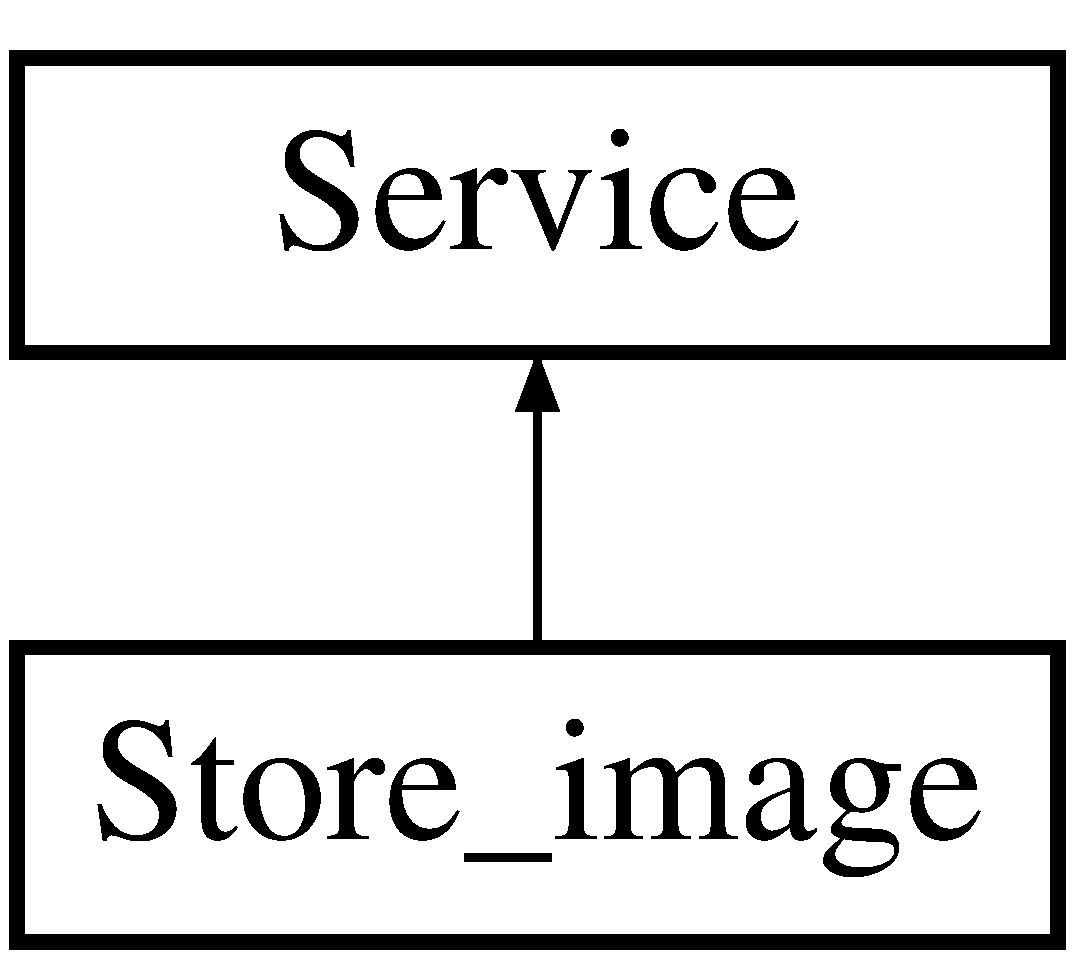
\includegraphics[height=2.000000cm]{class_store__image}
\end{center}
\end{figure}
\subsection*{Membri pubblici}
\begin{DoxyCompactItemize}
\item 
\hyperlink{class_store__image_a0aafc6c6b1b4576fe2de4d4a0feba356}{Store\-\_\-image} ()
\begin{DoxyCompactList}\small\item\em Costruttore di default della classe \hyperlink{class_store__image}{Store\-\_\-image}. \end{DoxyCompactList}\item 
\hyperlink{class_store__image_abb51b6465dd579b07268133b8c6dd8ef}{Store\-\_\-image} (string name, string address, string port)
\begin{DoxyCompactList}\small\item\em Costruttore che inizializza l'istanza della classe \hyperlink{class_store__image}{Store\-\_\-image} con i parametri forniti. \end{DoxyCompactList}\item 
\hyperlink{class_store__image_a5ac30f07f3db9fcbfc784ef79b6907c0}{Store\-\_\-image} (string name, string address, string port, string \hyperlink{class_store__image_ae7e32f8d0404e94e02a234ec54a17d70}{path})
\begin{DoxyCompactList}\small\item\em Costruttore che inizializza l'istanza della classe \hyperlink{class_store__image}{Store\-\_\-image} con i parametri forniti. \end{DoxyCompactList}\item 
\hyperlink{class_store__image_a2303ecf6c9d27ef0af198b27f924b460}{Store\-\_\-image} (\hyperlink{struct_service__description}{Service\-\_\-description} $\ast$\hyperlink{class_service_a55e991ff18c0dceca202388a771283dc}{s\-\_\-description})
\begin{DoxyCompactList}\small\item\em Costruttore che inizializza la classe \hyperlink{class_store__image}{Store\-\_\-image} con le informazioni ottenute dalla descrizione del servizio. \end{DoxyCompactList}\item 
\hyperlink{class_store__image_a89d05f2212b79d1aa5a297c217dc96cb}{Store\-\_\-image} (\hyperlink{struct_service__description}{Service\-\_\-description} $\ast$\hyperlink{class_service_a55e991ff18c0dceca202388a771283dc}{s\-\_\-description}, string \hyperlink{class_store__image_ae7e32f8d0404e94e02a234ec54a17d70}{path})
\begin{DoxyCompactList}\small\item\em Costruttore che inizializza la classe \hyperlink{class_store__image}{Store\-\_\-image} con le informazioni ottenute dalla descrizione del servizio e imposta la directory di lavoro con il path fornito in ingresso. \end{DoxyCompactList}\item 
\hypertarget{class_store__image_a8188f68bd84bf1408b1dd053392f005c}{virtual \hyperlink{class_store__image_a8188f68bd84bf1408b1dd053392f005c}{$\sim$\-Store\-\_\-image} ()}\label{class_store__image_a8188f68bd84bf1408b1dd053392f005c}

\begin{DoxyCompactList}\small\item\em Distruttore della classe \hyperlink{class_store__image}{Store\-\_\-image}. \end{DoxyCompactList}\item 
bool \hyperlink{class_store__image_a4023d6ecc72801dcbc52b30e89f17b2b}{execute} ()
\begin{DoxyCompactList}\small\item\em Genera una nuova immagine nella directory dello {\itshape Storage\-\_\-server} con nome e dati pari a quelli forniti in ingresso al servizio. \end{DoxyCompactList}\end{DoxyCompactItemize}
\subsection*{Membri privati}
\begin{DoxyCompactItemize}
\item 
void \hyperlink{class_store__image_a4156bdcb994ac460690dce12fbdeee79}{inizialize\-\_\-parameters} (string \hyperlink{class_store__image_ae7e32f8d0404e94e02a234ec54a17d70}{path})
\begin{DoxyCompactList}\small\item\em Inizializza l'istanza della classe \hyperlink{class_store__image}{Store\-\_\-image} (è chiamata da ogni costruttore). \end{DoxyCompactList}\end{DoxyCompactItemize}
\subsection*{Attributi privati}
\begin{DoxyCompactItemize}
\item 
\hypertarget{class_store__image_ae7e32f8d0404e94e02a234ec54a17d70}{string \hyperlink{class_store__image_ae7e32f8d0404e94e02a234ec54a17d70}{path}}\label{class_store__image_ae7e32f8d0404e94e02a234ec54a17d70}

\begin{DoxyCompactList}\small\item\em Directory di lavoro dello {\itshape Storage\-\_\-server} dove memorizzazione le immagini fornite dai {\itshape Clients}. \end{DoxyCompactList}\end{DoxyCompactItemize}
\subsection*{Altri membri ereditati}


\subsection{Descrizione dettagliata}
Classe che fornisce il servizio di memorizzazione di un immagine sul server remoto. E' una classe derivate di {\ttfamily \hyperlink{class_service}{Service}}. 

Definizione alla linea 97 del file Store\-\_\-image.\-h.



\subsection{Documentazione dei costruttori e dei distruttori}
\hypertarget{class_store__image_a0aafc6c6b1b4576fe2de4d4a0feba356}{\index{Store\-\_\-image@{Store\-\_\-image}!Store\-\_\-image@{Store\-\_\-image}}
\index{Store\-\_\-image@{Store\-\_\-image}!Store_image@{Store\-\_\-image}}
\subsubsection[{Store\-\_\-image}]{\setlength{\rightskip}{0pt plus 5cm}Store\-\_\-image\-::\-Store\-\_\-image (
\begin{DoxyParamCaption}
{}
\end{DoxyParamCaption}
)}}\label{class_store__image_a0aafc6c6b1b4576fe2de4d4a0feba356}


Costruttore di default della classe \hyperlink{class_store__image}{Store\-\_\-image}. 

Costruttore di default della classe \hyperlink{class_store__image}{Store\-\_\-image}. Provoca l'inizializzazione dei parametri di ingresso del servizio e setta la directory di lavoro sulla directory default. 

Definizione alla linea 5 del file Store\-\_\-image.\-cpp.

\hypertarget{class_store__image_abb51b6465dd579b07268133b8c6dd8ef}{\index{Store\-\_\-image@{Store\-\_\-image}!Store\-\_\-image@{Store\-\_\-image}}
\index{Store\-\_\-image@{Store\-\_\-image}!Store_image@{Store\-\_\-image}}
\subsubsection[{Store\-\_\-image}]{\setlength{\rightskip}{0pt plus 5cm}Store\-\_\-image\-::\-Store\-\_\-image (
\begin{DoxyParamCaption}
\item[{string}]{name, }
\item[{string}]{address, }
\item[{string}]{port}
\end{DoxyParamCaption}
)}}\label{class_store__image_abb51b6465dd579b07268133b8c6dd8ef}


Costruttore che inizializza l'istanza della classe \hyperlink{class_store__image}{Store\-\_\-image} con i parametri forniti. 


\begin{DoxyParams}[1]{Parametri}
\mbox{\tt in}  & {\em name} & Nome da assegnare al servizio. \\
\hline
\mbox{\tt in}  & {\em address} & Indirizzo I\-P del service provider che fornisce il servizio. \\
\hline
\mbox{\tt in}  & {\em port} & Porta di ascolto del service provider che fornisce il servizio. Costruttore che inizializza l'istanza della classe \hyperlink{class_store__image}{Store\-\_\-image} con nome, indirizzo e porta forniti in ingresso, inizializza i parametri di ingresso del servizio e setta la directory di lavoro sulla directory default. \\
\hline
\end{DoxyParams}


Definizione alla linea 9 del file Store\-\_\-image.\-cpp.

\hypertarget{class_store__image_a5ac30f07f3db9fcbfc784ef79b6907c0}{\index{Store\-\_\-image@{Store\-\_\-image}!Store\-\_\-image@{Store\-\_\-image}}
\index{Store\-\_\-image@{Store\-\_\-image}!Store_image@{Store\-\_\-image}}
\subsubsection[{Store\-\_\-image}]{\setlength{\rightskip}{0pt plus 5cm}Store\-\_\-image\-::\-Store\-\_\-image (
\begin{DoxyParamCaption}
\item[{string}]{name, }
\item[{string}]{address, }
\item[{string}]{port, }
\item[{string}]{path}
\end{DoxyParamCaption}
)}}\label{class_store__image_a5ac30f07f3db9fcbfc784ef79b6907c0}


Costruttore che inizializza l'istanza della classe \hyperlink{class_store__image}{Store\-\_\-image} con i parametri forniti. 


\begin{DoxyParams}[1]{Parametri}
\mbox{\tt in}  & {\em name} & Nome da assegnare al servizio. \\
\hline
\mbox{\tt in}  & {\em address} & Indirizzo I\-P del service provider che fornisce il servizio. \\
\hline
\mbox{\tt in}  & {\em port} & Porta di ascolto del service provider che fornisce il servizio. \\
\hline
\mbox{\tt in}  & {\em path} & Directory di lavoro da assegnare al servizio dove salvare i files temporanei. Costruttore che inizializza l'istanza della classe \hyperlink{class_store__image}{Store\-\_\-image} con nome, indirizzo e porta forniti in ingresso, inizializza i parametri di ingresso del servizio e imposta la directory di lavoro con il path fornito in ingresso. \\
\hline
\end{DoxyParams}


Definizione alla linea 12 del file Store\-\_\-image.\-cpp.

\hypertarget{class_store__image_a2303ecf6c9d27ef0af198b27f924b460}{\index{Store\-\_\-image@{Store\-\_\-image}!Store\-\_\-image@{Store\-\_\-image}}
\index{Store\-\_\-image@{Store\-\_\-image}!Store_image@{Store\-\_\-image}}
\subsubsection[{Store\-\_\-image}]{\setlength{\rightskip}{0pt plus 5cm}Store\-\_\-image\-::\-Store\-\_\-image (
\begin{DoxyParamCaption}
\item[{{\bf Service\-\_\-description} $\ast$}]{s\-\_\-description}
\end{DoxyParamCaption}
)}}\label{class_store__image_a2303ecf6c9d27ef0af198b27f924b460}


Costruttore che inizializza la classe \hyperlink{class_store__image}{Store\-\_\-image} con le informazioni ottenute dalla descrizione del servizio. 


\begin{DoxyParams}[1]{Parametri}
\mbox{\tt in}  & {\em s\-\_\-description} & Descrizione del servizio. \\
\hline
\end{DoxyParams}


Definizione alla linea 15 del file Store\-\_\-image.\-cpp.

\hypertarget{class_store__image_a89d05f2212b79d1aa5a297c217dc96cb}{\index{Store\-\_\-image@{Store\-\_\-image}!Store\-\_\-image@{Store\-\_\-image}}
\index{Store\-\_\-image@{Store\-\_\-image}!Store_image@{Store\-\_\-image}}
\subsubsection[{Store\-\_\-image}]{\setlength{\rightskip}{0pt plus 5cm}Store\-\_\-image\-::\-Store\-\_\-image (
\begin{DoxyParamCaption}
\item[{{\bf Service\-\_\-description} $\ast$}]{s\-\_\-description, }
\item[{string}]{path}
\end{DoxyParamCaption}
)}}\label{class_store__image_a89d05f2212b79d1aa5a297c217dc96cb}


Costruttore che inizializza la classe \hyperlink{class_store__image}{Store\-\_\-image} con le informazioni ottenute dalla descrizione del servizio e imposta la directory di lavoro con il path fornito in ingresso. 


\begin{DoxyParams}[1]{Parametri}
\mbox{\tt in}  & {\em s\-\_\-description} & Descrizione del servizio. \\
\hline
\mbox{\tt in}  & {\em path} & Directory di lavoro da assegnare al servizio dove salvare i files temporanei. \\
\hline
\end{DoxyParams}


Definizione alla linea 21 del file Store\-\_\-image.\-cpp.



\subsection{Documentazione delle funzioni membro}
\hypertarget{class_store__image_a4023d6ecc72801dcbc52b30e89f17b2b}{\index{Store\-\_\-image@{Store\-\_\-image}!execute@{execute}}
\index{execute@{execute}!Store_image@{Store\-\_\-image}}
\subsubsection[{execute}]{\setlength{\rightskip}{0pt plus 5cm}bool Store\-\_\-image\-::execute (
\begin{DoxyParamCaption}
{}
\end{DoxyParamCaption}
)\hspace{0.3cm}{\ttfamily [virtual]}}}\label{class_store__image_a4023d6ecc72801dcbc52b30e89f17b2b}


Genera una nuova immagine nella directory dello {\itshape Storage\-\_\-server} con nome e dati pari a quelli forniti in ingresso al servizio. 

\begin{DoxyReturn}{Restituisce}
Risultato dell'esecuzione, {\ttfamily true} in caso di successo e {\ttfamily false} altrimenti. 
\end{DoxyReturn}


Reimplementa \hyperlink{class_service}{Service}.



Definizione alla linea 39 del file Store\-\_\-image.\-cpp.

\hypertarget{class_store__image_a4156bdcb994ac460690dce12fbdeee79}{\index{Store\-\_\-image@{Store\-\_\-image}!inizialize\-\_\-parameters@{inizialize\-\_\-parameters}}
\index{inizialize\-\_\-parameters@{inizialize\-\_\-parameters}!Store_image@{Store\-\_\-image}}
\subsubsection[{inizialize\-\_\-parameters}]{\setlength{\rightskip}{0pt plus 5cm}Store\-\_\-image\-::inizialize\-\_\-parameters (
\begin{DoxyParamCaption}
\item[{string}]{path}
\end{DoxyParamCaption}
)\hspace{0.3cm}{\ttfamily [private]}}}\label{class_store__image_a4156bdcb994ac460690dce12fbdeee79}


Inizializza l'istanza della classe \hyperlink{class_store__image}{Store\-\_\-image} (è chiamata da ogni costruttore). 


\begin{DoxyParams}[1]{Parametri}
\mbox{\tt in}  & {\em path} & Directory di lavoro da assegnare al servizio dove salvare i files temporanei. Inizializza l'istanza della classe \hyperlink{class_store__image}{Store\-\_\-image} come segue\-: \begin{DoxyItemize}
\item genera un parametro in ingresso di tipo {\ttfamily string} che conterrà il nome con cui memorizzare l'immagine sul {\itshape Server} \item genera un parametro in ingresso di tipo {\ttfamily buffer} atto a mantenere le informazioni relative all'immagine da memorizzare \item crea la directory di lavoro del servizio se questa non esiste \end{DoxyItemize}
\\
\hline
\end{DoxyParams}


Definizione alla linea 30 del file Store\-\_\-image.\-cpp.



La documentazione per questa classe è stata generata a partire dai seguenti file\-:\begin{DoxyCompactItemize}
\item 
C\-:/\-Users/\-Matteo/\-Dropbox/\-Universita/\-Sistemi Operativi e Programmazione Distribuita/\-Progetto/\-Service\-\_\-\-Oriented\-\_\-\-Architecture/\-Sources/\-Application/\-Image\-\_\-storage\-\_\-server/\hyperlink{_store__image_8h}{Store\-\_\-image.\-h}\item 
C\-:/\-Users/\-Matteo/\-Dropbox/\-Universita/\-Sistemi Operativi e Programmazione Distribuita/\-Progetto/\-Service\-\_\-\-Oriented\-\_\-\-Architecture/\-Sources/\-Application/\-Image\-\_\-storage\-\_\-server/Store\-\_\-image.\-cpp\end{DoxyCompactItemize}

\hypertarget{class_threads}{\section{Riferimenti per la classe Threads}
\label{class_threads}\index{Threads@{Threads}}
}


Classe per la gestione dei threads di servizio e di controllo dei vari {\itshape Servers}.  




{\ttfamily \#include $<$Threads.\-h$>$}

\subsection*{Membri pubblici}
\begin{DoxyCompactItemize}
\item 
\hypertarget{class_threads_af2a22bb9473d2300df0797d0aa07e4bf}{\hyperlink{class_threads_af2a22bb9473d2300df0797d0aa07e4bf}{Threads} ()}\label{class_threads_af2a22bb9473d2300df0797d0aa07e4bf}

\begin{DoxyCompactList}\small\item\em Costruttore della classe \hyperlink{class_threads}{Threads}. Inizializza il semaforo e la variabile condition e setta il thread come attivo e libero. \end{DoxyCompactList}\item 
\hypertarget{class_threads_a2b4399a2f8fc2b507f118c27fba9eca4}{virtual \hyperlink{class_threads_a2b4399a2f8fc2b507f118c27fba9eca4}{$\sim$\-Threads} ()}\label{class_threads_a2b4399a2f8fc2b507f118c27fba9eca4}

\begin{DoxyCompactList}\small\item\em Distruttore della classe \hyperlink{class_threads}{Threads}. \end{DoxyCompactList}\item 
bool \hyperlink{class_threads_a46da5f5ed9ee3711f566dc6c4f608dd8}{test\-\_\-and\-\_\-set\-\_\-busy} ()
\begin{DoxyCompactList}\small\item\em Se il {\itshape thread} è libero lo setta come occupato altrimenti non effettua alcuna operazione e ritorna. \end{DoxyCompactList}\item 
\hypertarget{class_threads_a507afb25cd6e8b044e02150f57b43a85}{void \hyperlink{class_threads_a507afb25cd6e8b044e02150f57b43a85}{set\-\_\-busy} ()}\label{class_threads_a507afb25cd6e8b044e02150f57b43a85}

\begin{DoxyCompactList}\small\item\em Setta il {\itshape thread} su occupato. \end{DoxyCompactList}\item 
\hypertarget{class_threads_a06e59568497fd19f0fb115ffb40d25a5}{void \hyperlink{class_threads_a06e59568497fd19f0fb115ffb40d25a5}{set\-\_\-free} ()}\label{class_threads_a06e59568497fd19f0fb115ffb40d25a5}

\begin{DoxyCompactList}\small\item\em Setta il {\itshape thread} su libero. \end{DoxyCompactList}\item 
void \hyperlink{class_threads_a203c8939f82209d7d73ff4888f9de30e}{set\-\_\-socket} (int \hyperlink{class_threads_a5e30e204ecd4404d0f88514227b849a9}{client\-\_\-socket})
\begin{DoxyCompactList}\small\item\em Setta il {\itshape Socket} al valore passato come parametro. \end{DoxyCompactList}\item 
void \hyperlink{class_threads_ae976db915d6d729bf33b1368c9be191a}{set\-\_\-\-I\-D} (pthread\-\_\-t \hyperlink{class_threads_ab7e3c990d2c44c2352b4d9d682a5edaf}{thread\-\_\-\-I\-D})
\begin{DoxyCompactList}\small\item\em Setta l'identificativo del {\itshape thread} al valore passato come parametro. \end{DoxyCompactList}\item 
int \hyperlink{class_threads_a8c9867eae5ffe0142930e14f93194f82}{get\-\_\-socket} ()
\begin{DoxyCompactList}\small\item\em Ritorna al chiamante il {\itshape socket} associato al {\itshape thread}. \end{DoxyCompactList}\item 
pthread\-\_\-t \hyperlink{class_threads_ad044422afc205e16fb9104fe4cfa1a4f}{get\-\_\-\-I\-D} ()
\begin{DoxyCompactList}\small\item\em Ritorna al chiamante l'I\-D del {\itshape thread}. \end{DoxyCompactList}\item 
bool \hyperlink{class_threads_ad770694763602c65aa13388a380721c3}{is\-\_\-busy} ()
\begin{DoxyCompactList}\small\item\em Verifica se il {\itshape thread} è occupato o meno. \end{DoxyCompactList}\item 
bool \hyperlink{class_threads_ae56ff1063a0be830f73291b0e22a9c2b}{is\-\_\-active} ()
\begin{DoxyCompactList}\small\item\em Verifica se il {\itshape thread} è attivo o meno. \end{DoxyCompactList}\item 
\hypertarget{class_threads_a876bab16a1294650147391f9b294b522}{void \hyperlink{class_threads_a876bab16a1294650147391f9b294b522}{wait\-\_\-start} ()}\label{class_threads_a876bab16a1294650147391f9b294b522}

\begin{DoxyCompactList}\small\item\em Se il {\itshape thread} è libero si sospende in attesa dell'invocazione del metodo {\ttfamily \hyperlink{class_threads_aae72428047672adac8701f3986b84683}{thread\-\_\-start()}}. \end{DoxyCompactList}\item 
\hypertarget{class_threads_aae72428047672adac8701f3986b84683}{void \hyperlink{class_threads_aae72428047672adac8701f3986b84683}{thread\-\_\-start} ()}\label{class_threads_aae72428047672adac8701f3986b84683}

\begin{DoxyCompactList}\small\item\em Attiva il {\itshape thread} in attesa per servire una richiesta di un {\itshape Client}. \end{DoxyCompactList}\item 
\hypertarget{class_threads_aec60551054d334fb7d6c38471ebfd3bd}{void \hyperlink{class_threads_aec60551054d334fb7d6c38471ebfd3bd}{thread\-\_\-exit} ()}\label{class_threads_aec60551054d334fb7d6c38471ebfd3bd}

\begin{DoxyCompactList}\small\item\em Setta il {\itshape thread} su occupato e inattivo e lo sveglia per far terminare la sua esecuzione. \end{DoxyCompactList}\end{DoxyCompactItemize}
\subsection*{Attributi privati}
\begin{DoxyCompactItemize}
\item 
\hypertarget{class_threads_abed55b6a7e70edfb736b738bce7964d6}{bool \hyperlink{class_threads_abed55b6a7e70edfb736b738bce7964d6}{busy}}\label{class_threads_abed55b6a7e70edfb736b738bce7964d6}

\begin{DoxyCompactList}\small\item\em {\itshape Thread} occupato, viene impostato a {\ttfamily true} se il {\itshape thread} è stato associato ad un {\itshape Client} per rispondere ad una richiesta. \end{DoxyCompactList}\item 
\hypertarget{class_threads_a13f564c85b6bd2bc3bd39c12c612bb7a}{bool \hyperlink{class_threads_a13f564c85b6bd2bc3bd39c12c612bb7a}{active}}\label{class_threads_a13f564c85b6bd2bc3bd39c12c612bb7a}

\begin{DoxyCompactList}\small\item\em {\itshape Thread} attivo, viene impostato a {\ttfamily false} per terminare il {\itshape thread}. \end{DoxyCompactList}\item 
\hypertarget{class_threads_a5e30e204ecd4404d0f88514227b849a9}{int \hyperlink{class_threads_a5e30e204ecd4404d0f88514227b849a9}{client\-\_\-socket}}\label{class_threads_a5e30e204ecd4404d0f88514227b849a9}

\begin{DoxyCompactList}\small\item\em {\itshape Socket} associato al {\itshape thread} per dialogare con il {\itshape Client}. \end{DoxyCompactList}\item 
\hypertarget{class_threads_ab7e3c990d2c44c2352b4d9d682a5edaf}{pthread\-\_\-t \hyperlink{class_threads_ab7e3c990d2c44c2352b4d9d682a5edaf}{thread\-\_\-\-I\-D}}\label{class_threads_ab7e3c990d2c44c2352b4d9d682a5edaf}

\begin{DoxyCompactList}\small\item\em Identificativo del {\itshape thread}. \end{DoxyCompactList}\item 
\hypertarget{class_threads_afc98741291ee4f116654a90c0d26bc7b}{pthread\-\_\-mutex\-\_\-t \hyperlink{class_threads_afc98741291ee4f116654a90c0d26bc7b}{mutex}}\label{class_threads_afc98741291ee4f116654a90c0d26bc7b}

\begin{DoxyCompactList}\small\item\em {\itshape Semaforo} per l'accesso in mutua esclusione agli attributi della classe. \end{DoxyCompactList}\item 
\hypertarget{class_threads_a9ba05d7a4e514f04fd3aee99393d3c94}{pthread\-\_\-cond\-\_\-t \hyperlink{class_threads_a9ba05d7a4e514f04fd3aee99393d3c94}{condition}}\label{class_threads_a9ba05d7a4e514f04fd3aee99393d3c94}

\begin{DoxyCompactList}\small\item\em {\itshape Condizione} utilizzata per sospendere il {\itshape thread} in attesa di una richiesta da parte di un {\itshape Client}. \end{DoxyCompactList}\end{DoxyCompactItemize}


\subsection{Descrizione dettagliata}
Classe per la gestione dei threads di servizio e di controllo dei vari {\itshape Servers}. 

Definizione alla linea 101 del file Threads.\-h.



\subsection{Documentazione delle funzioni membro}
\hypertarget{class_threads_ad044422afc205e16fb9104fe4cfa1a4f}{\index{Threads@{Threads}!get\-\_\-\-I\-D@{get\-\_\-\-I\-D}}
\index{get\-\_\-\-I\-D@{get\-\_\-\-I\-D}!Threads@{Threads}}
\subsubsection[{get\-\_\-\-I\-D}]{\setlength{\rightskip}{0pt plus 5cm}pthread\-\_\-t Threads\-::get\-\_\-\-I\-D (
\begin{DoxyParamCaption}
{}
\end{DoxyParamCaption}
)}}\label{class_threads_ad044422afc205e16fb9104fe4cfa1a4f}


Ritorna al chiamante l'I\-D del {\itshape thread}. 

\begin{DoxyReturn}{Restituisce}
{\itshape Identificativo} associato al {\itshape thread}. 
\end{DoxyReturn}


Definizione alla linea 50 del file Threads.\-cpp.

\hypertarget{class_threads_a8c9867eae5ffe0142930e14f93194f82}{\index{Threads@{Threads}!get\-\_\-socket@{get\-\_\-socket}}
\index{get\-\_\-socket@{get\-\_\-socket}!Threads@{Threads}}
\subsubsection[{get\-\_\-socket}]{\setlength{\rightskip}{0pt plus 5cm}int Threads\-::get\-\_\-socket (
\begin{DoxyParamCaption}
{}
\end{DoxyParamCaption}
)}}\label{class_threads_a8c9867eae5ffe0142930e14f93194f82}


Ritorna al chiamante il {\itshape socket} associato al {\itshape thread}. 

\begin{DoxyReturn}{Restituisce}
{\itshape Socket} associato al {\itshape thread}. 
\end{DoxyReturn}


Definizione alla linea 46 del file Threads.\-cpp.

\hypertarget{class_threads_ae56ff1063a0be830f73291b0e22a9c2b}{\index{Threads@{Threads}!is\-\_\-active@{is\-\_\-active}}
\index{is\-\_\-active@{is\-\_\-active}!Threads@{Threads}}
\subsubsection[{is\-\_\-active}]{\setlength{\rightskip}{0pt plus 5cm}bool Threads\-::is\-\_\-active (
\begin{DoxyParamCaption}
{}
\end{DoxyParamCaption}
)}}\label{class_threads_ae56ff1063a0be830f73291b0e22a9c2b}


Verifica se il {\itshape thread} è attivo o meno. 

\begin{DoxyReturn}{Restituisce}
{\ttfamily true} se il {\itshape thread} è attivo e {\ttfamily false} altrimenti. 
\end{DoxyReturn}


Definizione alla linea 58 del file Threads.\-cpp.

\hypertarget{class_threads_ad770694763602c65aa13388a380721c3}{\index{Threads@{Threads}!is\-\_\-busy@{is\-\_\-busy}}
\index{is\-\_\-busy@{is\-\_\-busy}!Threads@{Threads}}
\subsubsection[{is\-\_\-busy}]{\setlength{\rightskip}{0pt plus 5cm}bool Threads\-::is\-\_\-busy (
\begin{DoxyParamCaption}
{}
\end{DoxyParamCaption}
)}}\label{class_threads_ad770694763602c65aa13388a380721c3}


Verifica se il {\itshape thread} è occupato o meno. 

\begin{DoxyReturn}{Restituisce}
{\ttfamily true} se il {\itshape thread} è occupato e {\ttfamily false} altrimenti. 
\end{DoxyReturn}


Definizione alla linea 54 del file Threads.\-cpp.

\hypertarget{class_threads_ae976db915d6d729bf33b1368c9be191a}{\index{Threads@{Threads}!set\-\_\-\-I\-D@{set\-\_\-\-I\-D}}
\index{set\-\_\-\-I\-D@{set\-\_\-\-I\-D}!Threads@{Threads}}
\subsubsection[{set\-\_\-\-I\-D}]{\setlength{\rightskip}{0pt plus 5cm}void Threads\-::set\-\_\-\-I\-D (
\begin{DoxyParamCaption}
\item[{pthread\-\_\-t}]{thread\-\_\-\-I\-D}
\end{DoxyParamCaption}
)}}\label{class_threads_ae976db915d6d729bf33b1368c9be191a}


Setta l'identificativo del {\itshape thread} al valore passato come parametro. 


\begin{DoxyParams}[1]{Parametri}
\mbox{\tt in}  & {\em thread\-\_\-\-I\-D} & I\-D da assegnare al {\itshape thread}. \\
\hline
\end{DoxyParams}


Definizione alla linea 40 del file Threads.\-cpp.

\hypertarget{class_threads_a203c8939f82209d7d73ff4888f9de30e}{\index{Threads@{Threads}!set\-\_\-socket@{set\-\_\-socket}}
\index{set\-\_\-socket@{set\-\_\-socket}!Threads@{Threads}}
\subsubsection[{set\-\_\-socket}]{\setlength{\rightskip}{0pt plus 5cm}void Threads\-::set\-\_\-socket (
\begin{DoxyParamCaption}
\item[{int}]{client\-\_\-socket}
\end{DoxyParamCaption}
)}}\label{class_threads_a203c8939f82209d7d73ff4888f9de30e}


Setta il {\itshape Socket} al valore passato come parametro. 


\begin{DoxyParams}[1]{Parametri}
\mbox{\tt in}  & {\em client\-\_\-socket} & {\itshape Socket} per l'interazione con il {\itshape Client}. \\
\hline
\end{DoxyParams}


Definizione alla linea 34 del file Threads.\-cpp.

\hypertarget{class_threads_a46da5f5ed9ee3711f566dc6c4f608dd8}{\index{Threads@{Threads}!test\-\_\-and\-\_\-set\-\_\-busy@{test\-\_\-and\-\_\-set\-\_\-busy}}
\index{test\-\_\-and\-\_\-set\-\_\-busy@{test\-\_\-and\-\_\-set\-\_\-busy}!Threads@{Threads}}
\subsubsection[{test\-\_\-and\-\_\-set\-\_\-busy}]{\setlength{\rightskip}{0pt plus 5cm}bool Threads\-::test\-\_\-and\-\_\-set\-\_\-busy (
\begin{DoxyParamCaption}
{}
\end{DoxyParamCaption}
)}}\label{class_threads_a46da5f5ed9ee3711f566dc6c4f608dd8}


Se il {\itshape thread} è libero lo setta come occupato altrimenti non effettua alcuna operazione e ritorna. 

\begin{DoxyReturn}{Restituisce}
{\ttfamily true} se il {\itshape thread} è stato settato come occupato (era libero al momento della chiamata) e {\ttfamily false} altrimenti. 
\end{DoxyReturn}


Definizione alla linea 13 del file Threads.\-cpp.



La documentazione per questa classe è stata generata a partire dai seguenti file\-:\begin{DoxyCompactItemize}
\item 
C\-:/\-Users/\-Matteo/\-Dropbox/\-Universita/\-Sistemi Operativi e Programmazione Distribuita/\-Progetto/\-Service\-\_\-\-Oriented\-\_\-\-Architecture/\-Sources/\-S\-O\-A\-\_\-\-Library/\hyperlink{_threads_8h}{Threads.\-h}\item 
C\-:/\-Users/\-Matteo/\-Dropbox/\-Universita/\-Sistemi Operativi e Programmazione Distribuita/\-Progetto/\-Service\-\_\-\-Oriented\-\_\-\-Architecture/\-Sources/\-S\-O\-A\-\_\-\-Library/Threads.\-cpp\end{DoxyCompactItemize}

\chapter{Documentazione dei file}
\hypertarget{_l_i_c_e_n_s_e_8md}{\section{Riferimenti per il file C\-:/\-Users/\-Matteo/\-Dropbox/\-Universita/\-Sistemi Operativi e Programmazione Distribuita/\-Progetto/\-Service\-\_\-\-Oriented\-\_\-\-Architecture/\-L\-I\-C\-E\-N\-S\-E.md}
\label{_l_i_c_e_n_s_e_8md}\index{C\-:/\-Users/\-Matteo/\-Dropbox/\-Universita/\-Sistemi Operativi e Programmazione Distribuita/\-Progetto/\-Service\-\_\-\-Oriented\-\_\-\-Architecture/\-L\-I\-C\-E\-N\-S\-E.\-md@{C\-:/\-Users/\-Matteo/\-Dropbox/\-Universita/\-Sistemi Operativi e Programmazione Distribuita/\-Progetto/\-Service\-\_\-\-Oriented\-\_\-\-Architecture/\-L\-I\-C\-E\-N\-S\-E.\-md}}
}


\subsection{Descrizione dettagliata}
\begin{DoxyDate}{Data}
15/05/2013 
\end{DoxyDate}
\begin{DoxyAuthor}{Autore}
Matteo Tamburini \href{mailto:mattetambu@gmail.com}{\tt mattetambu@gmail.\-com} 
\end{DoxyAuthor}
\begin{DoxyCopyright}{Copyright}
Copyright (c) 2013 Matteo Tamburini. All rights reserved. $\ast$/ 
\end{DoxyCopyright}


Definizione nel file \hyperlink{_l_i_c_e_n_s_e_8md_source}{L\-I\-C\-E\-N\-S\-E.\-md}.


\hypertarget{_horizontal__flip__image_8h}{\section{Riferimenti per il file C\-:/\-Users/\-Matteo/\-Dropbox/\-Universita/\-Sistemi Operativi e Programmazione Distribuita/\-Progetto/\-Service\-\_\-\-Oriented\-\_\-\-Architecture/\-Sources/\-Application/\-Image\-\_\-manipulation\-\_\-server/\-Horizontal\-\_\-flip\-\_\-image.h}
\label{_horizontal__flip__image_8h}\index{C\-:/\-Users/\-Matteo/\-Dropbox/\-Universita/\-Sistemi Operativi e Programmazione Distribuita/\-Progetto/\-Service\-\_\-\-Oriented\-\_\-\-Architecture/\-Sources/\-Application/\-Image\-\_\-manipulation\-\_\-server/\-Horizontal\-\_\-flip\-\_\-image.\-h@{C\-:/\-Users/\-Matteo/\-Dropbox/\-Universita/\-Sistemi Operativi e Programmazione Distribuita/\-Progetto/\-Service\-\_\-\-Oriented\-\_\-\-Architecture/\-Sources/\-Application/\-Image\-\_\-manipulation\-\_\-server/\-Horizontal\-\_\-flip\-\_\-image.\-h}}
}
{\ttfamily \#include \char`\"{}../../\-S\-O\-A\-\_\-\-Library/\-Service.\-h\char`\"{}}\\*
{\ttfamily \#include $<$Magick++.\-h$>$}\\*
{\ttfamily \#include $<$sstream$>$}\\*
\subsection*{Composti}
\begin{DoxyCompactItemize}
\item 
class \hyperlink{class_horizontal__flip__image}{Horizontal\-\_\-flip\-\_\-image}
\begin{DoxyCompactList}\small\item\em Classe che fornisce il servizio di riflessione di un immagine. E' una classe derivate di {\ttfamily \hyperlink{class_service}{Service}}. \end{DoxyCompactList}\end{DoxyCompactItemize}
\subsection*{Definizioni}
\begin{DoxyCompactItemize}
\item 
\hypertarget{_horizontal__flip__image_8h_a10c19941600f2d5487d3d0b9a4690b5e}{\#define \hyperlink{_horizontal__flip__image_8h_a10c19941600f2d5487d3d0b9a4690b5e}{F\-L\-I\-P\-\_\-\-I\-M\-A\-G\-E\-\_\-\-D\-I\-R\-E\-C\-T\-O\-R\-Y}~\char`\"{}./Work\-\_\-directories/Servers/Image\-\_\-manipulation\-\_\-server/\hyperlink{class_horizontal__flip__image}{Horizontal\-\_\-flip\-\_\-image}/\char`\"{}}\label{_horizontal__flip__image_8h_a10c19941600f2d5487d3d0b9a4690b5e}

\begin{DoxyCompactList}\small\item\em Directory di lavoro di default dove salvare i files temporanei (immagine sorgente e risultato della riflessione). \end{DoxyCompactList}\item 
\hypertarget{_horizontal__flip__image_8h_ad1680bda7ed4b6871b29ee99d7f3347b}{\#define \hyperlink{_horizontal__flip__image_8h_ad1680bda7ed4b6871b29ee99d7f3347b}{R\-E\-M\-O\-V\-E\-\_\-\-I\-M\-A\-G\-E\-S}~true}\label{_horizontal__flip__image_8h_ad1680bda7ed4b6871b29ee99d7f3347b}

\begin{DoxyCompactList}\small\item\em Se impostata a {\ttfamily true} provoca la rimozione dei files temporanei (immagine sorgente e risultato della riflessione) del {\itshape Server}. \end{DoxyCompactList}\end{DoxyCompactItemize}

\hypertarget{_image__manipulation__server__functions_8h}{\section{Riferimenti per il file C\-:/\-Users/\-Matteo/\-Dropbox/\-Universita/\-Sistemi Operativi e Programmazione Distribuita/\-Progetto/\-Service\-\_\-\-Oriented\-\_\-\-Architecture/\-Sources/\-Application/\-Image\-\_\-manipulation\-\_\-server/\-Image\-\_\-manipulation\-\_\-server\-\_\-functions.h}
\label{_image__manipulation__server__functions_8h}\index{C\-:/\-Users/\-Matteo/\-Dropbox/\-Universita/\-Sistemi Operativi e Programmazione Distribuita/\-Progetto/\-Service\-\_\-\-Oriented\-\_\-\-Architecture/\-Sources/\-Application/\-Image\-\_\-manipulation\-\_\-server/\-Image\-\_\-manipulation\-\_\-server\-\_\-functions.\-h@{C\-:/\-Users/\-Matteo/\-Dropbox/\-Universita/\-Sistemi Operativi e Programmazione Distribuita/\-Progetto/\-Service\-\_\-\-Oriented\-\_\-\-Architecture/\-Sources/\-Application/\-Image\-\_\-manipulation\-\_\-server/\-Image\-\_\-manipulation\-\_\-server\-\_\-functions.\-h}}
}
{\ttfamily \#include \char`\"{}../../\-S\-O\-A\-\_\-\-Library/\-Interface.\-h\char`\"{}}\\*
{\ttfamily \#include \char`\"{}../../\-S\-O\-A\-\_\-\-Library/\-Threads.\-h\char`\"{}}\\*
{\ttfamily \#include \char`\"{}./\-Horizontal\-\_\-flip\-\_\-image.\-h\char`\"{}}\\*
{\ttfamily \#include \char`\"{}./\-Rotate\-\_\-image.\-h\char`\"{}}\\*
\subsection*{Definizioni}
\begin{DoxyCompactItemize}
\item 
\hypertarget{_image__manipulation__server__functions_8h_ab60b5074c740fd36061f48f90d1a0b21}{\#define \hyperlink{_image__manipulation__server__functions_8h_ab60b5074c740fd36061f48f90d1a0b21}{N\-\_\-\-T\-H\-R\-E\-A\-D\-S}~5}\label{_image__manipulation__server__functions_8h_ab60b5074c740fd36061f48f90d1a0b21}

\begin{DoxyCompactList}\small\item\em Numero di {\itshape threads} di servizio da avviare. \end{DoxyCompactList}\item 
\hypertarget{_image__manipulation__server__functions_8h_a0e06fd5133b564b00c6cf5179b0c7dae}{\#define \hyperlink{_image__manipulation__server__functions_8h_a0e06fd5133b564b00c6cf5179b0c7dae}{B\-A\-C\-K\-L\-O\-G\-\_\-\-Q\-U\-E\-U\-E}~5}\label{_image__manipulation__server__functions_8h_a0e06fd5133b564b00c6cf5179b0c7dae}

\begin{DoxyCompactList}\small\item\em Dimensione della {\itshape backlog} {\itshape queue} associatta al {\itshape listen\-\_\-socket}. \end{DoxyCompactList}\end{DoxyCompactItemize}
\subsection*{Funzioni}
\begin{DoxyCompactItemize}
\item 
bool \hyperlink{_image__manipulation__server__functions_8h_a925117a2338469d636cae90df0071bca}{check\-\_\-server\-\_\-arguments} (int n\-\_\-args, char $\ast$$\ast$args)
\begin{DoxyCompactList}\small\item\em Controllo dei parametri della funzione main del {\itshape Server}. \end{DoxyCompactList}\item 
bool \hyperlink{_image__manipulation__server__functions_8h_a906def4577c8de63bd7e69ab67544b25}{assign\-\_\-execution\-\_\-thread} (int client\-\_\-socket)
\begin{DoxyCompactList}\small\item\em Cerca fra i {\itshape threads} di servizio un {\itshape thread} libero e lo assegna all'esecuzione della richiesta. \end{DoxyCompactList}\item 
\hypertarget{_image__manipulation__server__functions_8h_a63aac0df64e5330e61c9073bd0599b5a}{bool \hyperlink{_image__manipulation__server__functions_8h_a63aac0df64e5330e61c9073bd0599b5a}{Image\-\_\-manipulation\-\_\-server\-\_\-help} ()}\label{_image__manipulation__server__functions_8h_a63aac0df64e5330e61c9073bd0599b5a}

\begin{DoxyCompactList}\small\item\em Fornisce l'elenco dei comandi accettati dal {\itshape Server}. \end{DoxyCompactList}\item 
void $\ast$ \hyperlink{_image__manipulation__server__functions_8h_a6425f50e0cbc135c5c3d408150e75a10}{thread\-\_\-body} (void $\ast$thread\-\_\-\-I\-D)
\begin{DoxyCompactList}\small\item\em Corpo di tutti i {\itshape threads} di servizio dell' {\itshape Image\-\_\-manipulation\-\_\-server}. \end{DoxyCompactList}\item 
void $\ast$ \hyperlink{_image__manipulation__server__functions_8h_a784d39059165dac03a7efb9647721638}{control\-\_\-thread\-\_\-body} (void $\ast$)
\begin{DoxyCompactList}\small\item\em Corpo del {\itshape thread} di controllo dell' {\itshape Image\-\_\-manipulation\-\_\-server}. \end{DoxyCompactList}\end{DoxyCompactItemize}
\subsection*{Variabili}
\begin{DoxyCompactItemize}
\item 
\hypertarget{_image__manipulation__server__functions_8h_aca9046eb50925905ee659f62165684a8}{\hyperlink{class_rotate__image}{Rotate\-\_\-image} $\ast$ {\bfseries rotate\-\_\-image}}\label{_image__manipulation__server__functions_8h_aca9046eb50925905ee659f62165684a8}

\item 
\hypertarget{_image__manipulation__server__functions_8h_a13fcd89c5446b2b2fb0396dda88e1f2f}{\hyperlink{class_horizontal__flip__image}{Horizontal\-\_\-flip\-\_\-image} $\ast$ {\bfseries horizontal\-\_\-flip\-\_\-image}}\label{_image__manipulation__server__functions_8h_a13fcd89c5446b2b2fb0396dda88e1f2f}

\item 
\hypertarget{_image__manipulation__server__functions_8h_a0ed034ec7ce91872d20ac23938717979}{\hyperlink{class_threads}{Threads} {\bfseries thread} \mbox{[}\hyperlink{_service__register__server__functions_8h_ab60b5074c740fd36061f48f90d1a0b21}{N\-\_\-\-T\-H\-R\-E\-A\-D\-S}\mbox{]}}\label{_image__manipulation__server__functions_8h_a0ed034ec7ce91872d20ac23938717979}

\item 
\hypertarget{_image__manipulation__server__functions_8h_abfdf383881624687ed194172e80bcf24}{\hyperlink{class_threads}{Threads} {\bfseries control\-\_\-thread}}\label{_image__manipulation__server__functions_8h_abfdf383881624687ed194172e80bcf24}

\item 
\hypertarget{_image__manipulation__server__functions_8h_a559eb01bc152bcd6033e52d64f6e7c41}{pthread\-\_\-mutex\-\_\-t {\bfseries mutex\-\_\-thread\-\_\-free}}\label{_image__manipulation__server__functions_8h_a559eb01bc152bcd6033e52d64f6e7c41}

\item 
\hypertarget{_image__manipulation__server__functions_8h_a8b905b65075946d1d9fcaa813c86b9b3}{pthread\-\_\-cond\-\_\-t {\bfseries cond\-\_\-thread\-\_\-free}}\label{_image__manipulation__server__functions_8h_a8b905b65075946d1d9fcaa813c86b9b3}

\item 
\hypertarget{_image__manipulation__server__functions_8h_a943218f30384a427b7bd8da5ae257de3}{string {\bfseries S\-P\-\_\-address}}\label{_image__manipulation__server__functions_8h_a943218f30384a427b7bd8da5ae257de3}

\item 
\hypertarget{_image__manipulation__server__functions_8h_a6bc5fae6d25ed705c56d65ef46151964}{string {\bfseries S\-R\-\_\-address}}\label{_image__manipulation__server__functions_8h_a6bc5fae6d25ed705c56d65ef46151964}

\item 
\hypertarget{_image__manipulation__server__functions_8h_a37f86869479ef17f2f082e5d6dee8dbf}{string {\bfseries S\-P\-\_\-port}}\label{_image__manipulation__server__functions_8h_a37f86869479ef17f2f082e5d6dee8dbf}

\item 
\hypertarget{_image__manipulation__server__functions_8h_a1f02378765d968db00d5126f213e9038}{string {\bfseries S\-R\-\_\-port}}\label{_image__manipulation__server__functions_8h_a1f02378765d968db00d5126f213e9038}

\item 
\hypertarget{_image__manipulation__server__functions_8h_a28ab6dd809db802c37f5e6ab8a95db79}{int {\bfseries listen\-\_\-socket}}\label{_image__manipulation__server__functions_8h_a28ab6dd809db802c37f5e6ab8a95db79}

\end{DoxyCompactItemize}


\subsection{Documentazione delle funzioni}
\hypertarget{_image__manipulation__server__functions_8h_a906def4577c8de63bd7e69ab67544b25}{\index{Image\-\_\-manipulation\-\_\-server\-\_\-functions.\-h@{Image\-\_\-manipulation\-\_\-server\-\_\-functions.\-h}!assign\-\_\-execution\-\_\-thread@{assign\-\_\-execution\-\_\-thread}}
\index{assign\-\_\-execution\-\_\-thread@{assign\-\_\-execution\-\_\-thread}!Image_manipulation_server_functions.h@{Image\-\_\-manipulation\-\_\-server\-\_\-functions.\-h}}
\subsubsection[{assign\-\_\-execution\-\_\-thread}]{\setlength{\rightskip}{0pt plus 5cm}bool assign\-\_\-execution\-\_\-thread (
\begin{DoxyParamCaption}
\item[{int}]{client\-\_\-socket}
\end{DoxyParamCaption}
)}}\label{_image__manipulation__server__functions_8h_a906def4577c8de63bd7e69ab67544b25}


Cerca fra i {\itshape threads} di servizio un {\itshape thread} libero e lo assegna all'esecuzione della richiesta. 

\begin{DoxyReturn}{Restituisce}
{\ttfamily true} in caso di assegnamento eseguito con successo, {\ttfamily false} altrimenti (tutti i {\itshape threads} sono occupati). 
\end{DoxyReturn}


Definizione alla linea 117 del file Image\-\_\-manipulation\-\_\-server\-\_\-functions.\-h.

\hypertarget{_image__manipulation__server__functions_8h_a925117a2338469d636cae90df0071bca}{\index{Image\-\_\-manipulation\-\_\-server\-\_\-functions.\-h@{Image\-\_\-manipulation\-\_\-server\-\_\-functions.\-h}!check\-\_\-server\-\_\-arguments@{check\-\_\-server\-\_\-arguments}}
\index{check\-\_\-server\-\_\-arguments@{check\-\_\-server\-\_\-arguments}!Image_manipulation_server_functions.h@{Image\-\_\-manipulation\-\_\-server\-\_\-functions.\-h}}
\subsubsection[{check\-\_\-server\-\_\-arguments}]{\setlength{\rightskip}{0pt plus 5cm}bool check\-\_\-server\-\_\-arguments (
\begin{DoxyParamCaption}
\item[{int}]{n\-\_\-args, }
\item[{char $\ast$$\ast$}]{args}
\end{DoxyParamCaption}
)}}\label{_image__manipulation__server__functions_8h_a925117a2338469d636cae90df0071bca}


Controllo dei parametri della funzione main del {\itshape Server}. 


\begin{DoxyParams}[1]{Parametri}
\mbox{\tt in}  & {\em n\-\_\-args} & Numero di argomenti in ingresso al {\itshape Server}. \\
\hline
\mbox{\tt in}  & {\em args} & Array di argomenti in ingresso al {\itshape Server}. \\
\hline
\end{DoxyParams}
\begin{DoxyReturn}{Restituisce}
Risultato della verifica, {\ttfamily true} in caso di successo e {\ttfamily false} altrimenti. Al {\itshape Server} sono necessari tre parametri per la sua esecuzione e se viene invocato con un numero inferiore di argomenti questa funzione richiede l'inserimento di quelli mancanti. Il controllo sui parametri necessari al {\itshape Server} viene effettuato nel seguente modo\-: \begin{DoxyItemize}
\item il primo deve essere un intero nell'intervallo \mbox{[}1024-\/65535\mbox{]} e rappresenta la porta di ascolto dell' {\itshape Image\-\_\-manipulation\-\_\-server} \item il secondo deve essere un indirizzo I\-P e rappresenta l'indirizzo I\-P del {\itshape Service\-\_\-register\-\_\-server} \item il terzo deve essere un intero nell'intervallo \mbox{[}1024-\/65535\mbox{]} e rappresenta la porta di ascolto del {\itshape Service\-\_\-register\-\_\-server} \end{DoxyItemize}

\end{DoxyReturn}

\begin{DoxyParams}[1]{Parametri}
\mbox{\tt in}  & {\em n\-\_\-args} & Numero di argomenti in ingresso al {\itshape Server}. \\
\hline
\mbox{\tt in}  & {\em args} & Array di argomenti in ingresso al {\itshape Server}. \\
\hline
\end{DoxyParams}
\begin{DoxyReturn}{Restituisce}
Risultato della verifica, {\ttfamily true} in caso di successo e {\ttfamily false} altrimenti. Al {\itshape Server} sono necessari tre parametri per la sua esecuzione e se viene invocato con un numero inferiore di argomenti questa funzione richiede l'inserimento di quelli mancanti. Il controllo sui parametri necessari al {\itshape Server} viene effettuato nel seguente modo\-: \begin{DoxyItemize}
\item il primo deve essere un intero nell'intervallo \mbox{[}1024-\/65535\mbox{]} e rappresenta la porta di ascolto dell' {\itshape Image\-\_\-storage\-\_\-server} \item il secondo deve essere un indirizzo I\-P e rappresenta l'indirizzo I\-P del {\itshape Service\-\_\-register\-\_\-server} \item il terzo deve essere un intero nell'intervallo \mbox{[}1024-\/65535\mbox{]} e rappresenta la porta di ascolto del {\itshape Service\-\_\-register\-\_\-server} \end{DoxyItemize}

\end{DoxyReturn}

\begin{DoxyParams}[1]{Parametri}
\mbox{\tt in}  & {\em n\-\_\-args} & Numero di argomenti in ingresso al {\itshape Server}. \\
\hline
\mbox{\tt in}  & {\em args} & Array di argomenti in ingresso al {\itshape Server}. \\
\hline
\end{DoxyParams}
\begin{DoxyReturn}{Restituisce}
Risultato della verifica, {\ttfamily true} in caso di successo e {\ttfamily false} altrimenti. Al {\itshape Server} è necessario un solo parametro per la corretta esecuzione e se viene invocato privo di argomenti questa funzione ne richiede l'inserimento. Il parametro necessario al {\itshape Server} è un intero nell'intervallo \mbox{[}1024-\/65535\mbox{]} e rappresenta la porta di ascolto del {\itshape Service\-\_\-register\-\_\-server}. 
\end{DoxyReturn}


Definizione alla linea 90 del file Image\-\_\-manipulation\-\_\-server\-\_\-functions.\-h.

\hypertarget{_image__manipulation__server__functions_8h_a784d39059165dac03a7efb9647721638}{\index{Image\-\_\-manipulation\-\_\-server\-\_\-functions.\-h@{Image\-\_\-manipulation\-\_\-server\-\_\-functions.\-h}!control\-\_\-thread\-\_\-body@{control\-\_\-thread\-\_\-body}}
\index{control\-\_\-thread\-\_\-body@{control\-\_\-thread\-\_\-body}!Image_manipulation_server_functions.h@{Image\-\_\-manipulation\-\_\-server\-\_\-functions.\-h}}
\subsubsection[{control\-\_\-thread\-\_\-body}]{\setlength{\rightskip}{0pt plus 5cm}void $\ast$ control\-\_\-thread\-\_\-body (
\begin{DoxyParamCaption}
\item[{void $\ast$}]{}
\end{DoxyParamCaption}
)}}\label{_image__manipulation__server__functions_8h_a784d39059165dac03a7efb9647721638}


Corpo del {\itshape thread} di controllo dell' {\itshape Image\-\_\-manipulation\-\_\-server}. 

Corpo del {\itshape thread} di controllo del {\itshape Service\-\_\-register\-\_\-server}.

Corpo del {\itshape thread} di controllo dell' {\itshape Image\-\_\-storage\-\_\-server}.

Il {\itshape thread} di controllo, fino alla ricezione del comando di terminazione, esegue ciclicamente le seguenti operazioni\-: \begin{DoxyItemize}
\item si pone in attesa di essere attivato (manualmente) per eseguire un comando \item richiede l'inserimento del comando e verifica se è in grado di eseguirlo (altrimenti lo rifiuta) \item se il comando viene accettato esegue l'operazione corrispondente \end{DoxyItemize}


Definizione alla linea 184 del file Image\-\_\-manipulation\-\_\-server\-\_\-functions.\-h.

\hypertarget{_image__manipulation__server__functions_8h_a6425f50e0cbc135c5c3d408150e75a10}{\index{Image\-\_\-manipulation\-\_\-server\-\_\-functions.\-h@{Image\-\_\-manipulation\-\_\-server\-\_\-functions.\-h}!thread\-\_\-body@{thread\-\_\-body}}
\index{thread\-\_\-body@{thread\-\_\-body}!Image_manipulation_server_functions.h@{Image\-\_\-manipulation\-\_\-server\-\_\-functions.\-h}}
\subsubsection[{thread\-\_\-body}]{\setlength{\rightskip}{0pt plus 5cm}void $\ast$ thread\-\_\-body (
\begin{DoxyParamCaption}
\item[{void $\ast$}]{thread\-\_\-\-I\-D}
\end{DoxyParamCaption}
)}}\label{_image__manipulation__server__functions_8h_a6425f50e0cbc135c5c3d408150e75a10}


Corpo di tutti i {\itshape threads} di servizio dell' {\itshape Image\-\_\-manipulation\-\_\-server}. 

Corpo di tutti i {\itshape threads} di servizio del {\itshape Service\-\_\-register\-\_\-server}.

Corpo di tutti i {\itshape threads} di servizio dell' {\itshape Image\-\_\-storage\-\_\-server}.


\begin{DoxyParams}[1]{Parametri}
\mbox{\tt out}  & {\em thread\-\_\-\-I\-D} & Intero che identifica il {\itshape thread} a cui è associata l'istanza della funzione. Ogni {\itshape thread} di servizio, fino alla ricezione del comando di terminazione, esegue ciclicamente le seguenti operazioni\-: \begin{DoxyItemize}
\item segnala la sua disponibilità a ricevere connessioni e si pone in attesa di essere attivato per servire un {\itshape Client} \item riceve il nome del servizio richiesto dal {\itshape Client} e se questo non corrisponde ad un servizio fornito rifiuta al richiesta \item se la richiesta del {\itshape Client} viene accettata riceve i parametri necessari per l'esecuzione del servizio \item richiama il servizio richiesto (rotazione o riflessione dell'immagine) ottenendo il risultato della manipolazione \item invia al {\itshape Client} il risultato dell'esecuzione del servizio\end{DoxyItemize}
\\
\hline
\mbox{\tt in}  & {\em thread\-\_\-\-I\-D} & Intero che identifica il {\itshape thread} a cui è associata l'istanza della funzione. Ogni {\itshape thread} di servizio, fino alla ricezione del comando di terminazione, esegue ciclicamente le seguenti operazioni\-: \begin{DoxyItemize}
\item segnala la sua disponibilità a ricevere connessioni e si pone in attesa di essere attivato per servire un {\itshape Client} \item riceve il nome del servizio richiesto dal {\itshape Client} e se questo non corrisponde ad un servizio fornito rifiuta al richiesta \item se la richiesta del {\itshape Client} viene accettata riceve i parametri necessari per l'esecuzione del servizio \item richiama il servizio richiesto ed invia al {\itshape Client} il risultato dell'esecuzione\end{DoxyItemize}
\\
\hline
\mbox{\tt in}  & {\em thread\-\_\-\-I\-D} & Intero che identifica il {\itshape thread} a cui è associata l'istanza della funzione. Ogni {\itshape thread} di servizio, fino alla ricezione del comando di terminazione, esegue ciclicamente le seguenti operazioni\-: \begin{DoxyItemize}
\item segnala la sua disponibilità a ricevere connessioni e si pone in attesa di essere attivato per servire un {\itshape Client} \item riceve il nome del servizio richiesto dal {\itshape Client} e se questo non corrisponde ad un servizio fornito rifiuta al richiesta \item se la richiesta del {\itshape Client} viene accettata riceve i parametri necessari per l'esecuzione del servizio \item richiama il servizio richiesto e, se necessario, invia al {\itshape Client} il risultato dell'esecuzione \end{DoxyItemize}
\\
\hline
\end{DoxyParams}


Definizione alla linea 147 del file Image\-\_\-manipulation\-\_\-server\-\_\-functions.\-h.


\hypertarget{_rotate__image_8h}{\section{Riferimenti per il file C\-:/\-Users/\-Matteo/\-Dropbox/\-Universita/\-Sistemi Operativi e Programmazione Distribuita/\-Progetto/\-Service\-\_\-\-Oriented\-\_\-\-Architecture/\-Sources/\-Application/\-Image\-\_\-manipulation\-\_\-server/\-Rotate\-\_\-image.h}
\label{_rotate__image_8h}\index{C\-:/\-Users/\-Matteo/\-Dropbox/\-Universita/\-Sistemi Operativi e Programmazione Distribuita/\-Progetto/\-Service\-\_\-\-Oriented\-\_\-\-Architecture/\-Sources/\-Application/\-Image\-\_\-manipulation\-\_\-server/\-Rotate\-\_\-image.\-h@{C\-:/\-Users/\-Matteo/\-Dropbox/\-Universita/\-Sistemi Operativi e Programmazione Distribuita/\-Progetto/\-Service\-\_\-\-Oriented\-\_\-\-Architecture/\-Sources/\-Application/\-Image\-\_\-manipulation\-\_\-server/\-Rotate\-\_\-image.\-h}}
}
{\ttfamily \#include \char`\"{}../../\-S\-O\-A\-\_\-\-Library/\-Service.\-h\char`\"{}}\\*
{\ttfamily \#include $<$Magick++.\-h$>$}\\*
{\ttfamily \#include $<$sstream$>$}\\*
\subsection*{Composti}
\begin{DoxyCompactItemize}
\item 
class \hyperlink{class_rotate__image}{Rotate\-\_\-image}
\begin{DoxyCompactList}\small\item\em Classe che fornisce il servizio di rotazione di un immagine. E' una classe derivate di {\ttfamily \hyperlink{class_service}{Service}}. \end{DoxyCompactList}\end{DoxyCompactItemize}
\subsection*{Definizioni}
\begin{DoxyCompactItemize}
\item 
\hypertarget{_rotate__image_8h_a9954c3d0f9edeca7510d876320149261}{\#define \hyperlink{_rotate__image_8h_a9954c3d0f9edeca7510d876320149261}{R\-O\-T\-A\-T\-E\-\_\-\-I\-M\-A\-G\-E\-\_\-\-D\-I\-R\-E\-C\-T\-O\-R\-Y}~\char`\"{}./Work\-\_\-directories/Servers/Image\-\_\-manipulation\-\_\-server/\hyperlink{class_rotate__image}{Rotate\-\_\-image}/\char`\"{}}\label{_rotate__image_8h_a9954c3d0f9edeca7510d876320149261}

\begin{DoxyCompactList}\small\item\em Directory di lavoro di default dove salvare i files temporanei (immagine sorgente e risultato della rotazione). \end{DoxyCompactList}\item 
\hypertarget{_rotate__image_8h_ad1680bda7ed4b6871b29ee99d7f3347b}{\#define \hyperlink{_rotate__image_8h_ad1680bda7ed4b6871b29ee99d7f3347b}{R\-E\-M\-O\-V\-E\-\_\-\-I\-M\-A\-G\-E\-S}~true}\label{_rotate__image_8h_ad1680bda7ed4b6871b29ee99d7f3347b}

\begin{DoxyCompactList}\small\item\em Se impostata a {\ttfamily true} provoca la rimozione dei files temporanei (immagine sorgente e risultato della rotazione) del {\itshape Server}. \end{DoxyCompactList}\end{DoxyCompactItemize}

\hypertarget{_get__image_8h}{\section{Riferimenti per il file C\-:/\-Users/\-Matteo/\-Dropbox/\-Universita/\-Sistemi Operativi e Programmazione Distribuita/\-Progetto/\-Service\-\_\-\-Oriented\-\_\-\-Architecture/\-Sources/\-Application/\-Image\-\_\-storage\-\_\-server/\-Get\-\_\-image.h}
\label{_get__image_8h}\index{C\-:/\-Users/\-Matteo/\-Dropbox/\-Universita/\-Sistemi Operativi e Programmazione Distribuita/\-Progetto/\-Service\-\_\-\-Oriented\-\_\-\-Architecture/\-Sources/\-Application/\-Image\-\_\-storage\-\_\-server/\-Get\-\_\-image.\-h@{C\-:/\-Users/\-Matteo/\-Dropbox/\-Universita/\-Sistemi Operativi e Programmazione Distribuita/\-Progetto/\-Service\-\_\-\-Oriented\-\_\-\-Architecture/\-Sources/\-Application/\-Image\-\_\-storage\-\_\-server/\-Get\-\_\-image.\-h}}
}
{\ttfamily \#include \char`\"{}../../\-S\-O\-A\-\_\-\-Library/\-Service.\-h\char`\"{}}\\*
\subsection*{Composti}
\begin{DoxyCompactItemize}
\item 
class \hyperlink{class_get__image}{Get\-\_\-image}
\begin{DoxyCompactList}\small\item\em Classe che fornisce al richiedente un'immagine presente sul server remoto. E' una classe derivate di {\ttfamily \hyperlink{class_service}{Service}}. \end{DoxyCompactList}\end{DoxyCompactItemize}
\subsection*{Definizioni}
\begin{DoxyCompactItemize}
\item 
\hypertarget{_get__image_8h_ad46916667ab94241a554de462695aa06}{\#define \hyperlink{_get__image_8h_ad46916667ab94241a554de462695aa06}{G\-E\-T\-\_\-\-I\-M\-A\-G\-E\-\_\-\-D\-I\-R\-E\-C\-T\-O\-R\-Y}~\char`\"{}./Work\-\_\-directories/Servers/Image\-\_\-storage\-\_\-server/\char`\"{}}\label{_get__image_8h_ad46916667ab94241a554de462695aa06}

\begin{DoxyCompactList}\small\item\em Directory di default dello {\itshape Storage\-\_\-server} dove ricercare le immagini da fornire ai {\itshape Clients}. \end{DoxyCompactList}\end{DoxyCompactItemize}

\hypertarget{_get__list_8h}{\section{Riferimenti per il file C\-:/\-Users/\-Matteo/\-Dropbox/\-Universita/\-Sistemi Operativi e Programmazione Distribuita/\-Progetto/\-Service\-\_\-\-Oriented\-\_\-\-Architecture/\-Sources/\-Application/\-Image\-\_\-storage\-\_\-server/\-Get\-\_\-list.h}
\label{_get__list_8h}\index{C\-:/\-Users/\-Matteo/\-Dropbox/\-Universita/\-Sistemi Operativi e Programmazione Distribuita/\-Progetto/\-Service\-\_\-\-Oriented\-\_\-\-Architecture/\-Sources/\-Application/\-Image\-\_\-storage\-\_\-server/\-Get\-\_\-list.\-h@{C\-:/\-Users/\-Matteo/\-Dropbox/\-Universita/\-Sistemi Operativi e Programmazione Distribuita/\-Progetto/\-Service\-\_\-\-Oriented\-\_\-\-Architecture/\-Sources/\-Application/\-Image\-\_\-storage\-\_\-server/\-Get\-\_\-list.\-h}}
}
{\ttfamily \#include \char`\"{}../../\-S\-O\-A\-\_\-\-Library/\-Service.\-h\char`\"{}}\\*
\subsection*{Composti}
\begin{DoxyCompactItemize}
\item 
class \hyperlink{class_get__list}{Get\-\_\-list}
\begin{DoxyCompactList}\small\item\em Classe che fornisce la lista dei files presenti sul server remoto. E' una classe derivate di {\ttfamily \hyperlink{class_service}{Service}}. \end{DoxyCompactList}\end{DoxyCompactItemize}
\subsection*{Definizioni}
\begin{DoxyCompactItemize}
\item 
\hypertarget{_get__list_8h_a72b35caf6eb21053c326d497dc04f2a5}{\#define \hyperlink{_get__list_8h_a72b35caf6eb21053c326d497dc04f2a5}{G\-E\-T\-\_\-\-L\-I\-S\-T\-\_\-\-D\-I\-R\-E\-C\-T\-O\-R\-Y}~\char`\"{}./Work\-\_\-directories/Servers/Image\-\_\-storage\-\_\-server/\char`\"{}}\label{_get__list_8h_a72b35caf6eb21053c326d497dc04f2a5}

\begin{DoxyCompactList}\small\item\em Directory di default dello {\itshape Storage\-\_\-server} dove ricercare le immagini con cui creare la lista. \end{DoxyCompactList}\end{DoxyCompactItemize}

\hypertarget{_image__storage__server__functions_8h}{\section{Riferimenti per il file C\-:/\-Users/\-Matteo/\-Dropbox/\-Universita/\-Sistemi Operativi e Programmazione Distribuita/\-Progetto/\-Service\-\_\-\-Oriented\-\_\-\-Architecture/\-Sources/\-Application/\-Image\-\_\-storage\-\_\-server/\-Image\-\_\-storage\-\_\-server\-\_\-functions.h}
\label{_image__storage__server__functions_8h}\index{C\-:/\-Users/\-Matteo/\-Dropbox/\-Universita/\-Sistemi Operativi e Programmazione Distribuita/\-Progetto/\-Service\-\_\-\-Oriented\-\_\-\-Architecture/\-Sources/\-Application/\-Image\-\_\-storage\-\_\-server/\-Image\-\_\-storage\-\_\-server\-\_\-functions.\-h@{C\-:/\-Users/\-Matteo/\-Dropbox/\-Universita/\-Sistemi Operativi e Programmazione Distribuita/\-Progetto/\-Service\-\_\-\-Oriented\-\_\-\-Architecture/\-Sources/\-Application/\-Image\-\_\-storage\-\_\-server/\-Image\-\_\-storage\-\_\-server\-\_\-functions.\-h}}
}
{\ttfamily \#include \char`\"{}../../\-S\-O\-A\-\_\-\-Library/\-Interface.\-h\char`\"{}}\\*
{\ttfamily \#include \char`\"{}../../\-S\-O\-A\-\_\-\-Library/\-Threads.\-h\char`\"{}}\\*
{\ttfamily \#include \char`\"{}./\-Store\-\_\-image.\-h\char`\"{}}\\*
{\ttfamily \#include \char`\"{}./\-Get\-\_\-image.\-h\char`\"{}}\\*
{\ttfamily \#include \char`\"{}./\-Get\-\_\-list.\-h\char`\"{}}\\*
\subsection*{Definizioni}
\begin{DoxyCompactItemize}
\item 
\hypertarget{_image__storage__server__functions_8h_ab60b5074c740fd36061f48f90d1a0b21}{\#define \hyperlink{_image__storage__server__functions_8h_ab60b5074c740fd36061f48f90d1a0b21}{N\-\_\-\-T\-H\-R\-E\-A\-D\-S}~5}\label{_image__storage__server__functions_8h_ab60b5074c740fd36061f48f90d1a0b21}

\begin{DoxyCompactList}\small\item\em Numero di {\itshape threads} di servizio da avviare. \end{DoxyCompactList}\item 
\hypertarget{_image__storage__server__functions_8h_a0e06fd5133b564b00c6cf5179b0c7dae}{\#define \hyperlink{_image__storage__server__functions_8h_a0e06fd5133b564b00c6cf5179b0c7dae}{B\-A\-C\-K\-L\-O\-G\-\_\-\-Q\-U\-E\-U\-E}~5}\label{_image__storage__server__functions_8h_a0e06fd5133b564b00c6cf5179b0c7dae}

\begin{DoxyCompactList}\small\item\em Dimensione della {\itshape backlog} {\itshape queue} associatta al {\itshape listen\-\_\-socket}. \end{DoxyCompactList}\end{DoxyCompactItemize}
\subsection*{Funzioni}
\begin{DoxyCompactItemize}
\item 
\hypertarget{_image__storage__server__functions_8h_a925117a2338469d636cae90df0071bca}{bool {\bfseries check\-\_\-server\-\_\-arguments} (int n\-\_\-args, char $\ast$$\ast$args)}\label{_image__storage__server__functions_8h_a925117a2338469d636cae90df0071bca}

\item 
\hypertarget{_image__storage__server__functions_8h_a4718029e9211d4bf5cde09494f6de797}{void \hyperlink{_image__storage__server__functions_8h_a4718029e9211d4bf5cde09494f6de797}{readers\-\_\-prologue} ()}\label{_image__storage__server__functions_8h_a4718029e9211d4bf5cde09494f6de797}

\begin{DoxyCompactList}\small\item\em Se i files sono occupati da uno scrittore attende il turno dei lettori, altrimenti occupa i files permettendone l'accesso ai soli i lettori. \end{DoxyCompactList}\item 
\hypertarget{_image__storage__server__functions_8h_ac415b039a370332fef36036b0dd726fe}{void \hyperlink{_image__storage__server__functions_8h_ac415b039a370332fef36036b0dd726fe}{readers\-\_\-epilogue} ()}\label{_image__storage__server__functions_8h_ac415b039a370332fef36036b0dd726fe}

\begin{DoxyCompactList}\small\item\em Segnala la fine dell'elaborazione del {\itshape thread} lettore e se questo è l'ultimo lettore attivo rilascia la mutua esclusione. \end{DoxyCompactList}\item 
\hypertarget{_image__storage__server__functions_8h_a6864397834edf8a9c125a41696807340}{void \hyperlink{_image__storage__server__functions_8h_a6864397834edf8a9c125a41696807340}{writers\-\_\-prologue} ()}\label{_image__storage__server__functions_8h_a6864397834edf8a9c125a41696807340}

\begin{DoxyCompactList}\small\item\em Attende il proprio turno per l'accesso ai files che deve avvenire in mutua esclusione. \end{DoxyCompactList}\item 
\hypertarget{_image__storage__server__functions_8h_ab254aa378de15eb906ec5bf94dad0d02}{void \hyperlink{_image__storage__server__functions_8h_ab254aa378de15eb906ec5bf94dad0d02}{writers\-\_\-epilogue} ()}\label{_image__storage__server__functions_8h_ab254aa378de15eb906ec5bf94dad0d02}

\begin{DoxyCompactList}\small\item\em Segnala la fine dell'elaborazione del {\itshape thread} scrittore e rilascia la mutua esclusione. \end{DoxyCompactList}\item 
\hypertarget{_image__storage__server__functions_8h_a906def4577c8de63bd7e69ab67544b25}{bool {\bfseries assign\-\_\-execution\-\_\-thread} (int client\-\_\-socket)}\label{_image__storage__server__functions_8h_a906def4577c8de63bd7e69ab67544b25}

\item 
\hypertarget{_image__storage__server__functions_8h_a7ab376e8d3c9b090ad457f3a415d9bd9}{bool \hyperlink{_image__storage__server__functions_8h_a7ab376e8d3c9b090ad457f3a415d9bd9}{Image\-\_\-storage\-\_\-server\-\_\-help} ()}\label{_image__storage__server__functions_8h_a7ab376e8d3c9b090ad457f3a415d9bd9}

\begin{DoxyCompactList}\small\item\em Fornisce l'elenco dei comandi accettati dal {\itshape Server}. \end{DoxyCompactList}\item 
\hypertarget{_image__storage__server__functions_8h_ac4398e0b3dfc60215e7e66059d0cc3b8}{void $\ast$ {\bfseries thread\-\_\-body} (void $\ast$thread\-\_\-\-I\-D)}\label{_image__storage__server__functions_8h_ac4398e0b3dfc60215e7e66059d0cc3b8}

\item 
\hypertarget{_image__storage__server__functions_8h_ac158e4ccedf3add20952c9028e337631}{void $\ast$ {\bfseries control\-\_\-thread\-\_\-body} (void $\ast$)}\label{_image__storage__server__functions_8h_ac158e4ccedf3add20952c9028e337631}

\end{DoxyCompactItemize}
\subsection*{Variabili}
\begin{DoxyCompactItemize}
\item 
\hypertarget{_image__storage__server__functions_8h_a1b208f3b84c6035fee37ebb830538840}{\hyperlink{class_store__image}{Store\-\_\-image} $\ast$ {\bfseries store\-\_\-image}}\label{_image__storage__server__functions_8h_a1b208f3b84c6035fee37ebb830538840}

\item 
\hypertarget{_image__storage__server__functions_8h_abb59c88a9792d304c55184cc7cc0f52b}{\hyperlink{class_get__image}{Get\-\_\-image} $\ast$ {\bfseries get\-\_\-image}}\label{_image__storage__server__functions_8h_abb59c88a9792d304c55184cc7cc0f52b}

\item 
\hypertarget{_image__storage__server__functions_8h_a2a0da763f6570be9ef5ec17bb5dfb3a8}{\hyperlink{class_get__list}{Get\-\_\-list} $\ast$ {\bfseries get\-\_\-list}}\label{_image__storage__server__functions_8h_a2a0da763f6570be9ef5ec17bb5dfb3a8}

\item 
\hypertarget{_image__storage__server__functions_8h_a0ed034ec7ce91872d20ac23938717979}{\hyperlink{class_threads}{Threads} {\bfseries thread} \mbox{[}\hyperlink{_service__register__server__functions_8h_ab60b5074c740fd36061f48f90d1a0b21}{N\-\_\-\-T\-H\-R\-E\-A\-D\-S}\mbox{]}}\label{_image__storage__server__functions_8h_a0ed034ec7ce91872d20ac23938717979}

\item 
\hypertarget{_image__storage__server__functions_8h_abfdf383881624687ed194172e80bcf24}{\hyperlink{class_threads}{Threads} {\bfseries control\-\_\-thread}}\label{_image__storage__server__functions_8h_abfdf383881624687ed194172e80bcf24}

\item 
\hypertarget{_image__storage__server__functions_8h_a76f671dd42a5d3616c3b7ddb567fa49f}{pthread\-\_\-mutex\-\_\-t {\bfseries mutex\-\_\-1}}\label{_image__storage__server__functions_8h_a76f671dd42a5d3616c3b7ddb567fa49f}

\item 
\hypertarget{_image__storage__server__functions_8h_ab2169e1ab92dbdce252b6780691d5bab}{pthread\-\_\-mutex\-\_\-t {\bfseries mutex\-\_\-2}}\label{_image__storage__server__functions_8h_ab2169e1ab92dbdce252b6780691d5bab}

\item 
\hypertarget{_image__storage__server__functions_8h_a559eb01bc152bcd6033e52d64f6e7c41}{pthread\-\_\-mutex\-\_\-t {\bfseries mutex\-\_\-thread\-\_\-free}}\label{_image__storage__server__functions_8h_a559eb01bc152bcd6033e52d64f6e7c41}

\item 
\hypertarget{_image__storage__server__functions_8h_a8b905b65075946d1d9fcaa813c86b9b3}{pthread\-\_\-cond\-\_\-t {\bfseries cond\-\_\-thread\-\_\-free}}\label{_image__storage__server__functions_8h_a8b905b65075946d1d9fcaa813c86b9b3}

\item 
\hypertarget{_image__storage__server__functions_8h_a943218f30384a427b7bd8da5ae257de3}{string {\bfseries S\-P\-\_\-address}}\label{_image__storage__server__functions_8h_a943218f30384a427b7bd8da5ae257de3}

\item 
\hypertarget{_image__storage__server__functions_8h_a6bc5fae6d25ed705c56d65ef46151964}{string {\bfseries S\-R\-\_\-address}}\label{_image__storage__server__functions_8h_a6bc5fae6d25ed705c56d65ef46151964}

\item 
\hypertarget{_image__storage__server__functions_8h_a37f86869479ef17f2f082e5d6dee8dbf}{string {\bfseries S\-P\-\_\-port}}\label{_image__storage__server__functions_8h_a37f86869479ef17f2f082e5d6dee8dbf}

\item 
\hypertarget{_image__storage__server__functions_8h_a1f02378765d968db00d5126f213e9038}{string {\bfseries S\-R\-\_\-port}}\label{_image__storage__server__functions_8h_a1f02378765d968db00d5126f213e9038}

\item 
\hypertarget{_image__storage__server__functions_8h_a28ab6dd809db802c37f5e6ab8a95db79}{int {\bfseries listen\-\_\-socket}}\label{_image__storage__server__functions_8h_a28ab6dd809db802c37f5e6ab8a95db79}

\item 
\hypertarget{_image__storage__server__functions_8h_afd6c40de3c12fd6c40c3b32883e5605f}{int {\bfseries readers\-\_\-count} = 0}\label{_image__storage__server__functions_8h_afd6c40de3c12fd6c40c3b32883e5605f}

\end{DoxyCompactItemize}

\hypertarget{_store__image_8h}{\section{Riferimenti per il file C\-:/\-Users/\-Matteo/\-Dropbox/\-Universita/\-Sistemi Operativi e Programmazione Distribuita/\-Progetto/\-Service\-\_\-\-Oriented\-\_\-\-Architecture/\-Sources/\-Application/\-Image\-\_\-storage\-\_\-server/\-Store\-\_\-image.h}
\label{_store__image_8h}\index{C\-:/\-Users/\-Matteo/\-Dropbox/\-Universita/\-Sistemi Operativi e Programmazione Distribuita/\-Progetto/\-Service\-\_\-\-Oriented\-\_\-\-Architecture/\-Sources/\-Application/\-Image\-\_\-storage\-\_\-server/\-Store\-\_\-image.\-h@{C\-:/\-Users/\-Matteo/\-Dropbox/\-Universita/\-Sistemi Operativi e Programmazione Distribuita/\-Progetto/\-Service\-\_\-\-Oriented\-\_\-\-Architecture/\-Sources/\-Application/\-Image\-\_\-storage\-\_\-server/\-Store\-\_\-image.\-h}}
}
{\ttfamily \#include \char`\"{}../../\-S\-O\-A\-\_\-\-Library/\-Service.\-h\char`\"{}}\\*
\subsection*{Composti}
\begin{DoxyCompactItemize}
\item 
class \hyperlink{class_store__image}{Store\-\_\-image}
\begin{DoxyCompactList}\small\item\em Classe che fornisce il servizio di memorizzazione di un immagine sul server remoto. E' una classe derivate di {\ttfamily \hyperlink{class_service}{Service}}. \end{DoxyCompactList}\end{DoxyCompactItemize}
\subsection*{Definizioni}
\begin{DoxyCompactItemize}
\item 
\hypertarget{_store__image_8h_a77418f1a67c49011707a52b4699d1e01}{\#define \hyperlink{_store__image_8h_a77418f1a67c49011707a52b4699d1e01}{S\-T\-O\-R\-E\-\_\-\-I\-M\-A\-G\-E\-\_\-\-D\-I\-R\-E\-C\-T\-O\-R\-Y}~\char`\"{}./Work\-\_\-directories/Servers/Image\-\_\-storage\-\_\-server/\char`\"{}}\label{_store__image_8h_a77418f1a67c49011707a52b4699d1e01}

\begin{DoxyCompactList}\small\item\em Directory di default dello {\itshape Storage\-\_\-server} dove memorizzazione le immagini fornite dai {\itshape Clients}. \end{DoxyCompactList}\end{DoxyCompactItemize}

\hypertarget{_service__register_8h}{\section{Riferimenti per il file C\-:/\-Users/\-Matteo/\-Dropbox/\-Universita/\-Sistemi Operativi e Programmazione Distribuita/\-Progetto/\-Service\-\_\-\-Oriented\-\_\-\-Architecture/\-Sources/\-Application/\-Service\-\_\-register\-\_\-server/\-Service\-\_\-register.h}
\label{_service__register_8h}\index{C\-:/\-Users/\-Matteo/\-Dropbox/\-Universita/\-Sistemi Operativi e Programmazione Distribuita/\-Progetto/\-Service\-\_\-\-Oriented\-\_\-\-Architecture/\-Sources/\-Application/\-Service\-\_\-register\-\_\-server/\-Service\-\_\-register.\-h@{C\-:/\-Users/\-Matteo/\-Dropbox/\-Universita/\-Sistemi Operativi e Programmazione Distribuita/\-Progetto/\-Service\-\_\-\-Oriented\-\_\-\-Architecture/\-Sources/\-Application/\-Service\-\_\-register\-\_\-server/\-Service\-\_\-register.\-h}}
}
{\ttfamily \#include \char`\"{}../../\-S\-O\-A\-\_\-\-Library/\-Types.\-h\char`\"{}}\\*
{\ttfamily \#include $<$map$>$}\\*
{\ttfamily \#include $<$list$>$}\\*
{\ttfamily \#include $<$utility$>$}\\*
\subsection*{Composti}
\begin{DoxyCompactItemize}
\item 
class \hyperlink{class_service__register}{Service\-\_\-register}
\begin{DoxyCompactList}\small\item\em Classe che implementa il registro dei servizi. Qui vengono registrati i servizi forniti dai vari service provider. \end{DoxyCompactList}\end{DoxyCompactItemize}

\hypertarget{_service__register__server__functions_8h}{\section{Riferimenti per il file C\-:/\-Users/\-Matteo/\-Dropbox/\-Universita/\-Sistemi Operativi e Programmazione Distribuita/\-Progetto/\-Service\-\_\-\-Oriented\-\_\-\-Architecture/\-Sources/\-Application/\-Service\-\_\-register\-\_\-server/\-Service\-\_\-register\-\_\-server\-\_\-functions.h}
\label{_service__register__server__functions_8h}\index{C\-:/\-Users/\-Matteo/\-Dropbox/\-Universita/\-Sistemi Operativi e Programmazione Distribuita/\-Progetto/\-Service\-\_\-\-Oriented\-\_\-\-Architecture/\-Sources/\-Application/\-Service\-\_\-register\-\_\-server/\-Service\-\_\-register\-\_\-server\-\_\-functions.\-h@{C\-:/\-Users/\-Matteo/\-Dropbox/\-Universita/\-Sistemi Operativi e Programmazione Distribuita/\-Progetto/\-Service\-\_\-\-Oriented\-\_\-\-Architecture/\-Sources/\-Application/\-Service\-\_\-register\-\_\-server/\-Service\-\_\-register\-\_\-server\-\_\-functions.\-h}}
}
{\ttfamily \#include \char`\"{}../../\-S\-O\-A\-\_\-\-Library/\-Interface.\-h\char`\"{}}\\*
{\ttfamily \#include \char`\"{}../../\-S\-O\-A\-\_\-\-Library/\-Threads.\-h\char`\"{}}\\*
{\ttfamily \#include \char`\"{}./\-Service\-\_\-register.\-h\char`\"{}}\\*
\subsection*{Definizioni}
\begin{DoxyCompactItemize}
\item 
\hypertarget{_service__register__server__functions_8h_ab60b5074c740fd36061f48f90d1a0b21}{\#define \hyperlink{_service__register__server__functions_8h_ab60b5074c740fd36061f48f90d1a0b21}{N\-\_\-\-T\-H\-R\-E\-A\-D\-S}~5}\label{_service__register__server__functions_8h_ab60b5074c740fd36061f48f90d1a0b21}

\begin{DoxyCompactList}\small\item\em Numero di {\itshape threads} di servizio da avviare. \end{DoxyCompactList}\item 
\hypertarget{_service__register__server__functions_8h_a0e06fd5133b564b00c6cf5179b0c7dae}{\#define \hyperlink{_service__register__server__functions_8h_a0e06fd5133b564b00c6cf5179b0c7dae}{B\-A\-C\-K\-L\-O\-G\-\_\-\-Q\-U\-E\-U\-E}~5}\label{_service__register__server__functions_8h_a0e06fd5133b564b00c6cf5179b0c7dae}

\begin{DoxyCompactList}\small\item\em Dimensione della {\itshape backlog} {\itshape queue} associatta al {\itshape listen\-\_\-socket}. \end{DoxyCompactList}\end{DoxyCompactItemize}
\subsection*{Funzioni}
\begin{DoxyCompactItemize}
\item 
\hypertarget{_service__register__server__functions_8h_a925117a2338469d636cae90df0071bca}{bool {\bfseries check\-\_\-server\-\_\-arguments} (int n\-\_\-args, char $\ast$$\ast$args)}\label{_service__register__server__functions_8h_a925117a2338469d636cae90df0071bca}

\item 
\hypertarget{_service__register__server__functions_8h_a906def4577c8de63bd7e69ab67544b25}{bool {\bfseries assign\-\_\-execution\-\_\-thread} (int client\-\_\-socket)}\label{_service__register__server__functions_8h_a906def4577c8de63bd7e69ab67544b25}

\item 
\hypertarget{_service__register__server__functions_8h_aaf8bc61fa2ce7a323870c122834c2fbc}{bool \hyperlink{_service__register__server__functions_8h_aaf8bc61fa2ce7a323870c122834c2fbc}{Service\-\_\-register\-\_\-server\-\_\-help} ()}\label{_service__register__server__functions_8h_aaf8bc61fa2ce7a323870c122834c2fbc}

\begin{DoxyCompactList}\small\item\em Fornisce l'elenco dei comandi accettati dal {\itshape Server}. \end{DoxyCompactList}\item 
\hypertarget{_service__register__server__functions_8h_ac4398e0b3dfc60215e7e66059d0cc3b8}{void $\ast$ {\bfseries thread\-\_\-body} (void $\ast$thread\-\_\-\-I\-D)}\label{_service__register__server__functions_8h_ac4398e0b3dfc60215e7e66059d0cc3b8}

\item 
\hypertarget{_service__register__server__functions_8h_ac158e4ccedf3add20952c9028e337631}{void $\ast$ {\bfseries control\-\_\-thread\-\_\-body} (void $\ast$)}\label{_service__register__server__functions_8h_ac158e4ccedf3add20952c9028e337631}

\end{DoxyCompactItemize}
\subsection*{Variabili}
\begin{DoxyCompactItemize}
\item 
\hypertarget{_service__register__server__functions_8h_abe67addcb34733b89b2cca51e0ef5df7}{\hyperlink{class_service__register}{Service\-\_\-register} $\ast$ {\bfseries service\-\_\-register} = new \hyperlink{class_service__register}{Service\-\_\-register}()}\label{_service__register__server__functions_8h_abe67addcb34733b89b2cca51e0ef5df7}

\item 
\hypertarget{_service__register__server__functions_8h_a0ed034ec7ce91872d20ac23938717979}{\hyperlink{class_threads}{Threads} {\bfseries thread} \mbox{[}\hyperlink{_service__register__server__functions_8h_ab60b5074c740fd36061f48f90d1a0b21}{N\-\_\-\-T\-H\-R\-E\-A\-D\-S}\mbox{]}}\label{_service__register__server__functions_8h_a0ed034ec7ce91872d20ac23938717979}

\item 
\hypertarget{_service__register__server__functions_8h_abfdf383881624687ed194172e80bcf24}{\hyperlink{class_threads}{Threads} {\bfseries control\-\_\-thread}}\label{_service__register__server__functions_8h_abfdf383881624687ed194172e80bcf24}

\item 
\hypertarget{_service__register__server__functions_8h_a559eb01bc152bcd6033e52d64f6e7c41}{pthread\-\_\-mutex\-\_\-t {\bfseries mutex\-\_\-thread\-\_\-free}}\label{_service__register__server__functions_8h_a559eb01bc152bcd6033e52d64f6e7c41}

\item 
\hypertarget{_service__register__server__functions_8h_a8b905b65075946d1d9fcaa813c86b9b3}{pthread\-\_\-cond\-\_\-t {\bfseries cond\-\_\-thread\-\_\-free}}\label{_service__register__server__functions_8h_a8b905b65075946d1d9fcaa813c86b9b3}

\item 
\hypertarget{_service__register__server__functions_8h_a6bc5fae6d25ed705c56d65ef46151964}{string {\bfseries S\-R\-\_\-address}}\label{_service__register__server__functions_8h_a6bc5fae6d25ed705c56d65ef46151964}

\item 
\hypertarget{_service__register__server__functions_8h_a1f02378765d968db00d5126f213e9038}{string {\bfseries S\-R\-\_\-port}}\label{_service__register__server__functions_8h_a1f02378765d968db00d5126f213e9038}

\item 
\hypertarget{_service__register__server__functions_8h_a28ab6dd809db802c37f5e6ab8a95db79}{int {\bfseries listen\-\_\-socket}}\label{_service__register__server__functions_8h_a28ab6dd809db802c37f5e6ab8a95db79}

\end{DoxyCompactItemize}

\hypertarget{_client_8cpp}{\section{Riferimenti per il file C\-:/\-Users/\-Matteo/\-Dropbox/\-Universita/\-Sistemi Operativi e Programmazione Distribuita/\-Progetto/\-Service\-\_\-\-Oriented\-\_\-\-Architecture/\-Sources/\-Client.cpp}
\label{_client_8cpp}\index{C\-:/\-Users/\-Matteo/\-Dropbox/\-Universita/\-Sistemi Operativi e Programmazione Distribuita/\-Progetto/\-Service\-\_\-\-Oriented\-\_\-\-Architecture/\-Sources/\-Client.\-cpp@{C\-:/\-Users/\-Matteo/\-Dropbox/\-Universita/\-Sistemi Operativi e Programmazione Distribuita/\-Progetto/\-Service\-\_\-\-Oriented\-\_\-\-Architecture/\-Sources/\-Client.\-cpp}}
}
{\ttfamily \#include \char`\"{}./\-Application/\-Clients/\-Clients\-\_\-functions.\-h\char`\"{}}\\*
\subsection*{Funzioni}
\begin{DoxyCompactItemize}
\item 
int \hyperlink{_client_8cpp_a22577c6525b3f2fefecc0c741ba46a9a}{main} (int n\-\_\-args, char $\ast$$\ast$args)
\begin{DoxyCompactList}\small\item\em Corpo del {\itshape Client}. \end{DoxyCompactList}\end{DoxyCompactItemize}


\subsection{Documentazione delle funzioni}
\hypertarget{_client_8cpp_a22577c6525b3f2fefecc0c741ba46a9a}{\index{Client.\-cpp@{Client.\-cpp}!main@{main}}
\index{main@{main}!Client.cpp@{Client.\-cpp}}
\subsubsection[{main}]{\setlength{\rightskip}{0pt plus 5cm}int main (
\begin{DoxyParamCaption}
\item[{int}]{n\-\_\-args, }
\item[{char $\ast$$\ast$}]{args}
\end{DoxyParamCaption}
)}}\label{_client_8cpp_a22577c6525b3f2fefecc0c741ba46a9a}


Corpo del {\itshape Client}. 

Corpo del {\itshape Service\-\_\-register\-\_\-server}.

Corpo dell' {\itshape Image\-\_\-storage\-\_\-server}.

Corpo dell' {\itshape Image\-\_\-manipulation\-\_\-server}.


\begin{DoxyParams}[1]{Parametri}
\mbox{\tt in}  & {\em n\-\_\-args} & Numero di argomenti in ingresso al {\itshape Client}. \\
\hline
\mbox{\tt in}  & {\em args} & Array di argomenti in ingresso al {\itshape Client}. \\
\hline
\end{DoxyParams}
\begin{DoxyReturn}{Restituisce}
Risultato dell'esecuzione, {\ttfamily 0} in caso di successo e {\ttfamily -\/1} altrimenti. Il {\itshape Client} ciclicamente esegue le seguenti operazioni\-: \begin{DoxyItemize}
\item sceglie a caso un'immagine da disco o la richiede al service provider \item sceglie a caso un servizio di manipolazione da applicare all'immagine (rotazione o riflessione) e lo richiede al server \item invia il risultato della manipolazione al service provider per il salvataggio.\end{DoxyItemize}

\end{DoxyReturn}

\begin{DoxyParams}[1]{Parametri}
\mbox{\tt in}  & {\em n\-\_\-args} & Numero di argomenti in ingresso. \\
\hline
\mbox{\tt in}  & {\em args} & Array di argomenti in ingresso. \\
\hline
\end{DoxyParams}
\begin{DoxyReturn}{Restituisce}
Risultato dell'esecuzione, {\ttfamily 0} in caso di successo e {\ttfamily -\/1} altrimenti. L' {\itshape Image\-\_\-manipulation\-\_\-server} esegue le seguenti operazioni\-: \begin{DoxyItemize}
\item inizializza e crea un {\itshape socket} sul quale attendere le richieste di servizio \item registra i servizi offerti al {\itshape Service\-\_\-register\-\_\-server} \item inizializza e crea un insieme di {\itshape threads} di servizio che si occuperanno dell'esecuzione dei servizi richiesti \item inizializza e crea un {\itshape thread} di controllo che permette la gestione manuale del server attraverso appositi comandi \item ciclicamente si pone in attesa di richieste di servizio che, una volta accettate, assegna ad uno dei {\itshape threads} di servizio liberi \item ricevuto il comando di terminazione chiude le comunicazioni, deregistra i servizi e termina i threads precedentemente avviati, quindi termina a sua volta\end{DoxyItemize}

\end{DoxyReturn}

\begin{DoxyParams}[1]{Parametri}
\mbox{\tt in}  & {\em n\-\_\-args} & Numero di argomenti in ingresso. \\
\hline
\mbox{\tt in}  & {\em args} & Array di argomenti in ingresso. \\
\hline
\end{DoxyParams}
\begin{DoxyReturn}{Restituisce}
Risultato dell'esecuzione, {\ttfamily 0} in caso di successo e {\ttfamily -\/1} altrimenti. L' {\itshape Image\-\_\-storage\-\_\-server} esegue le seguenti operazioni\-: \begin{DoxyItemize}
\item inizializza e crea un {\itshape socket} sul quale attendere le richieste di servizio \item registra i servizi offerti al {\itshape Service\-\_\-register\-\_\-server} \item inizializza e crea un insieme di {\itshape threads} di servizio che si occuperanno dell'esecuzione dei servizi richiesti \item inizializza e crea un {\itshape thread} di controllo che permette la gestione manuale del server attraverso appositi comandi \item ciclicamente si pone in attesa di richieste di servizio che, una volta accettate, assegna ad uno dei {\itshape threads} di servizio liberi \item ricevuto il comando di terminazione chiude le comunicazioni, deregistra i servizi e termina i threads precedentemente avviati, quindi termina a sua volta\end{DoxyItemize}

\end{DoxyReturn}

\begin{DoxyParams}[1]{Parametri}
\mbox{\tt in}  & {\em n\-\_\-args} & Numero di argomenti in ingresso. \\
\hline
\mbox{\tt in}  & {\em args} & Array di argomenti in ingresso. \\
\hline
\end{DoxyParams}
\begin{DoxyReturn}{Restituisce}
Risultato dell'esecuzione, {\ttfamily 0} in caso di successo e {\ttfamily -\/1} altrimenti. Il {\itshape Service\-\_\-register\-\_\-server} esegue le seguenti operazioni\-: \begin{DoxyItemize}
\item inizializza e crea un {\itshape socket} sul quale attendere le richieste di servizio \item inizializza e crea un insieme di {\itshape threads} di servizio che si occuperanno dell'esecuzione dei servizi richiesti \item inizializza e crea un {\itshape thread} di controllo che permette la gestione manuale del server attraverso appositi comandi \item ciclicamente si pone in attesa di richieste di servizio che, una volta accettate, assegna ad uno dei {\itshape threads} di servizio liberi \item ricevuto il comando di terminazione chiude le comunicazioni e termina i threads precedentemente avviati, quindi termina a sua volta \end{DoxyItemize}

\end{DoxyReturn}


Definizione alla linea 27 del file Client.\-cpp.


\hypertarget{_image__manipulation__server_8cpp}{\section{Riferimenti per il file C\-:/\-Users/\-Matteo/\-Dropbox/\-Universita/\-Sistemi Operativi e Programmazione Distribuita/\-Progetto/\-Service\-\_\-\-Oriented\-\_\-\-Architecture/\-Sources/\-Image\-\_\-manipulation\-\_\-server.cpp}
\label{_image__manipulation__server_8cpp}\index{C\-:/\-Users/\-Matteo/\-Dropbox/\-Universita/\-Sistemi Operativi e Programmazione Distribuita/\-Progetto/\-Service\-\_\-\-Oriented\-\_\-\-Architecture/\-Sources/\-Image\-\_\-manipulation\-\_\-server.\-cpp@{C\-:/\-Users/\-Matteo/\-Dropbox/\-Universita/\-Sistemi Operativi e Programmazione Distribuita/\-Progetto/\-Service\-\_\-\-Oriented\-\_\-\-Architecture/\-Sources/\-Image\-\_\-manipulation\-\_\-server.\-cpp}}
}
{\ttfamily \#include \char`\"{}./\-Application/\-Image\-\_\-manipulation\-\_\-server/\-Image\-\_\-manipulation\-\_\-server\-\_\-functions.\-h\char`\"{}}\\*
\subsection*{Funzioni}
\begin{DoxyCompactItemize}
\item 
\hypertarget{_image__manipulation__server_8cpp_a22577c6525b3f2fefecc0c741ba46a9a}{int {\bfseries main} (int n\-\_\-args, char $\ast$$\ast$args)}\label{_image__manipulation__server_8cpp_a22577c6525b3f2fefecc0c741ba46a9a}

\end{DoxyCompactItemize}

\hypertarget{_image__storage__server_8cpp}{\section{Riferimenti per il file C\-:/\-Users/\-Matteo/\-Dropbox/\-Universita/\-Sistemi Operativi e Programmazione Distribuita/\-Progetto/\-Service\-\_\-\-Oriented\-\_\-\-Architecture/\-Sources/\-Image\-\_\-storage\-\_\-server.cpp}
\label{_image__storage__server_8cpp}\index{C\-:/\-Users/\-Matteo/\-Dropbox/\-Universita/\-Sistemi Operativi e Programmazione Distribuita/\-Progetto/\-Service\-\_\-\-Oriented\-\_\-\-Architecture/\-Sources/\-Image\-\_\-storage\-\_\-server.\-cpp@{C\-:/\-Users/\-Matteo/\-Dropbox/\-Universita/\-Sistemi Operativi e Programmazione Distribuita/\-Progetto/\-Service\-\_\-\-Oriented\-\_\-\-Architecture/\-Sources/\-Image\-\_\-storage\-\_\-server.\-cpp}}
}
{\ttfamily \#include \char`\"{}./\-Application/\-Image\-\_\-storage\-\_\-server/\-Image\-\_\-storage\-\_\-server\-\_\-functions.\-h\char`\"{}}\\*
\subsection*{Funzioni}
\begin{DoxyCompactItemize}
\item 
\hypertarget{_image__storage__server_8cpp_a22577c6525b3f2fefecc0c741ba46a9a}{int {\bfseries main} (int n\-\_\-args, char $\ast$$\ast$args)}\label{_image__storage__server_8cpp_a22577c6525b3f2fefecc0c741ba46a9a}

\end{DoxyCompactItemize}

\hypertarget{_service__register__server_8cpp}{\section{Riferimenti per il file C\-:/\-Users/\-Matteo/\-Dropbox/\-Universita/\-Sistemi Operativi e Programmazione Distribuita/\-Progetto/\-Service\-\_\-\-Oriented\-\_\-\-Architecture/\-Sources/\-Service\-\_\-register\-\_\-server.cpp}
\label{_service__register__server_8cpp}\index{C\-:/\-Users/\-Matteo/\-Dropbox/\-Universita/\-Sistemi Operativi e Programmazione Distribuita/\-Progetto/\-Service\-\_\-\-Oriented\-\_\-\-Architecture/\-Sources/\-Service\-\_\-register\-\_\-server.\-cpp@{C\-:/\-Users/\-Matteo/\-Dropbox/\-Universita/\-Sistemi Operativi e Programmazione Distribuita/\-Progetto/\-Service\-\_\-\-Oriented\-\_\-\-Architecture/\-Sources/\-Service\-\_\-register\-\_\-server.\-cpp}}
}
{\ttfamily \#include \char`\"{}./\-Application/\-Service\-\_\-register\-\_\-server/\-Service\-\_\-register\-\_\-server\-\_\-functions.\-h\char`\"{}}\\*
\subsection*{Funzioni}
\begin{DoxyCompactItemize}
\item 
\hypertarget{_service__register__server_8cpp_a22577c6525b3f2fefecc0c741ba46a9a}{int {\bfseries main} (int n\-\_\-args, char $\ast$$\ast$args)}\label{_service__register__server_8cpp_a22577c6525b3f2fefecc0c741ba46a9a}

\end{DoxyCompactItemize}

\hypertarget{_files__manager_8h}{\section{Riferimenti per il file C\-:/\-Users/\-Matteo/\-Dropbox/\-Universita/\-Sistemi Operativi e Programmazione Distribuita/\-Progetto/\-Service\-\_\-\-Oriented\-\_\-\-Architecture/\-Sources/\-S\-O\-A\-\_\-\-Library/\-Files\-\_\-manager.h}
\label{_files__manager_8h}\index{C\-:/\-Users/\-Matteo/\-Dropbox/\-Universita/\-Sistemi Operativi e Programmazione Distribuita/\-Progetto/\-Service\-\_\-\-Oriented\-\_\-\-Architecture/\-Sources/\-S\-O\-A\-\_\-\-Library/\-Files\-\_\-manager.\-h@{C\-:/\-Users/\-Matteo/\-Dropbox/\-Universita/\-Sistemi Operativi e Programmazione Distribuita/\-Progetto/\-Service\-\_\-\-Oriented\-\_\-\-Architecture/\-Sources/\-S\-O\-A\-\_\-\-Library/\-Files\-\_\-manager.\-h}}
}
{\ttfamily \#include \char`\"{}Types.\-h\char`\"{}}\\*
{\ttfamily \#include $<$dirent.\-h$>$}\\*
{\ttfamily \#include $<$sys/stat.\-h$>$}\\*
{\ttfamily \#include $<$sstream$>$}\\*
\subsection*{Funzioni}
\begin{DoxyCompactItemize}
\item 
string \hyperlink{_files__manager_8h_ab928e3f4581e827eef587ce75513837f}{make\-\_\-client\-\_\-working\-\_\-directory} (string path)
\begin{DoxyCompactList}\small\item\em Creazione della directory privata del {\itshape Client}. \end{DoxyCompactList}\item 
bool \hyperlink{_files__manager_8h_a8f124bfa05f27b19ac6c18911f7675bb}{make\-\_\-file\-\_\-list} (string path, vector$<$ string $>$ $\ast$file\-\_\-list)
\begin{DoxyCompactList}\small\item\em Crea una lista dei files presenti nella cartella specificata (tralasciando sottocartelle e files nascosti). \end{DoxyCompactList}\item 
bool \hyperlink{_files__manager_8h_a875101f39b6c8689c42787721893083c}{make\-\_\-image\-\_\-from\-\_\-buffer} (string image\-\_\-path, \hyperlink{structbuffer}{buffer} $\ast$image\-\_\-buffer)
\begin{DoxyCompactList}\small\item\em Crea un file al path specificato a partire dal buffer passato come parametro. \end{DoxyCompactList}\item 
bool \hyperlink{_files__manager_8h_af5f86e4f5008dadde00a35bfc0fd9e82}{get\-\_\-buffer\-\_\-from\-\_\-image} (string image\-\_\-path, \hyperlink{structbuffer}{buffer} $\ast$image\-\_\-buffer)
\begin{DoxyCompactList}\small\item\em Realizza un buffer a partire dal corpo di un file il cui path è passato come parametro. \end{DoxyCompactList}\end{DoxyCompactItemize}


\subsection{Documentazione delle funzioni}
\hypertarget{_files__manager_8h_af5f86e4f5008dadde00a35bfc0fd9e82}{\index{Files\-\_\-manager.\-h@{Files\-\_\-manager.\-h}!get\-\_\-buffer\-\_\-from\-\_\-image@{get\-\_\-buffer\-\_\-from\-\_\-image}}
\index{get\-\_\-buffer\-\_\-from\-\_\-image@{get\-\_\-buffer\-\_\-from\-\_\-image}!Files_manager.h@{Files\-\_\-manager.\-h}}
\subsubsection[{get\-\_\-buffer\-\_\-from\-\_\-image}]{\setlength{\rightskip}{0pt plus 5cm}bool get\-\_\-buffer\-\_\-from\-\_\-image (
\begin{DoxyParamCaption}
\item[{string}]{image\-\_\-path, }
\item[{{\bf buffer} $\ast$}]{image\-\_\-buffer}
\end{DoxyParamCaption}
)}}\label{_files__manager_8h_af5f86e4f5008dadde00a35bfc0fd9e82}


Realizza un buffer a partire dal corpo di un file il cui path è passato come parametro. 


\begin{DoxyParams}[1]{Parametri}
\mbox{\tt in}  & {\em image\-\_\-path} & Path relativo all'immagine da analizzare (comprensivo di nome ed estensione del file). \\
\hline
\mbox{\tt out}  & {\em image\-\_\-buffer} & Buffer che dovrà contenere il corpo del file. \\
\hline
\end{DoxyParams}
\begin{DoxyReturn}{Restituisce}
Risultato della lettura del file, {\ttfamily true} in caso di successo e {\ttfamily false} altrimenti. I dati relativi alla lettura del file il cui path (che contiene anche il nome e l'estensione del file) è passato come parametro sono inseriti all'interno del buffer specificato dal chiamante. 
\end{DoxyReturn}


Definizione alla linea 68 del file Files\-\_\-manager.\-cpp.

\hypertarget{_files__manager_8h_ab928e3f4581e827eef587ce75513837f}{\index{Files\-\_\-manager.\-h@{Files\-\_\-manager.\-h}!make\-\_\-client\-\_\-working\-\_\-directory@{make\-\_\-client\-\_\-working\-\_\-directory}}
\index{make\-\_\-client\-\_\-working\-\_\-directory@{make\-\_\-client\-\_\-working\-\_\-directory}!Files_manager.h@{Files\-\_\-manager.\-h}}
\subsubsection[{make\-\_\-client\-\_\-working\-\_\-directory}]{\setlength{\rightskip}{0pt plus 5cm}string make\-\_\-client\-\_\-working\-\_\-directory (
\begin{DoxyParamCaption}
\item[{string}]{path}
\end{DoxyParamCaption}
)}}\label{_files__manager_8h_ab928e3f4581e827eef587ce75513837f}


Creazione della directory privata del {\itshape Client}. 


\begin{DoxyParams}[1]{Parametri}
\mbox{\tt in}  & {\em path} & Directory di lavoro dei {\itshape Clients} all'interno della deve essere creata la directory privata. \\
\hline
\end{DoxyParams}
\begin{DoxyReturn}{Restituisce}
Indice identificativo del {\itshape Client} in caso di successo e una stringa vuota altrimenti. 
\end{DoxyReturn}


Definizione alla linea 4 del file Files\-\_\-manager.\-cpp.

\hypertarget{_files__manager_8h_a8f124bfa05f27b19ac6c18911f7675bb}{\index{Files\-\_\-manager.\-h@{Files\-\_\-manager.\-h}!make\-\_\-file\-\_\-list@{make\-\_\-file\-\_\-list}}
\index{make\-\_\-file\-\_\-list@{make\-\_\-file\-\_\-list}!Files_manager.h@{Files\-\_\-manager.\-h}}
\subsubsection[{make\-\_\-file\-\_\-list}]{\setlength{\rightskip}{0pt plus 5cm}bool make\-\_\-file\-\_\-list (
\begin{DoxyParamCaption}
\item[{string}]{path, }
\item[{vector$<$ string $>$ $\ast$}]{file\-\_\-list}
\end{DoxyParamCaption}
)}}\label{_files__manager_8h_a8f124bfa05f27b19ac6c18911f7675bb}


Crea una lista dei files presenti nella cartella specificata (tralasciando sottocartelle e files nascosti). 


\begin{DoxyParams}[1]{Parametri}
\mbox{\tt in}  & {\em path} & Directory di cui si richiede la lista di files. \\
\hline
\mbox{\tt out}  & {\em file\-\_\-list} & Vettore in cui inserire la lista di files. \\
\hline
\end{DoxyParams}
\begin{DoxyReturn}{Restituisce}
Risultato dell'esecuzione, {\ttfamily true} in caso di successo e {\ttfamily false} altrimenti. 
\end{DoxyReturn}


Definizione alla linea 23 del file Files\-\_\-manager.\-cpp.

\hypertarget{_files__manager_8h_a875101f39b6c8689c42787721893083c}{\index{Files\-\_\-manager.\-h@{Files\-\_\-manager.\-h}!make\-\_\-image\-\_\-from\-\_\-buffer@{make\-\_\-image\-\_\-from\-\_\-buffer}}
\index{make\-\_\-image\-\_\-from\-\_\-buffer@{make\-\_\-image\-\_\-from\-\_\-buffer}!Files_manager.h@{Files\-\_\-manager.\-h}}
\subsubsection[{make\-\_\-image\-\_\-from\-\_\-buffer}]{\setlength{\rightskip}{0pt plus 5cm}bool make\-\_\-image\-\_\-from\-\_\-buffer (
\begin{DoxyParamCaption}
\item[{string}]{image\-\_\-path, }
\item[{{\bf buffer} $\ast$}]{image\-\_\-buffer}
\end{DoxyParamCaption}
)}}\label{_files__manager_8h_a875101f39b6c8689c42787721893083c}


Crea un file al path specificato a partire dal buffer passato come parametro. 


\begin{DoxyParams}[1]{Parametri}
\mbox{\tt in}  & {\em image\-\_\-path} & Path relativo all'immagine da realizzare (comprensivo di nome ed estensione del file). \\
\hline
\mbox{\tt in}  & {\em image\-\_\-buffer} & Buffer contenente i dati dell'immagine da realizzare. \\
\hline
\end{DoxyParams}
\begin{DoxyReturn}{Restituisce}
Risultato della creazione del file, {\ttfamily true} in caso di successo e {\ttfamily false} altrimenti. Il buffer passato come parametro è utilizzato per dar corpo al file da realizzare che viene creato nella directory specificata dall'attributo path (che contiene anche il nome e l'estensione del file da creare) 
\end{DoxyReturn}


Definizione alla linea 40 del file Files\-\_\-manager.\-cpp.


\hypertarget{_interface_8h}{\section{Riferimenti per il file C\-:/\-Users/\-Matteo/\-Dropbox/\-Universita/\-Sistemi Operativi e Programmazione Distribuita/\-Progetto/\-Service\-\_\-\-Oriented\-\_\-\-Architecture/\-Sources/\-S\-O\-A\-\_\-\-Library/\-Interface.h}
\label{_interface_8h}\index{C\-:/\-Users/\-Matteo/\-Dropbox/\-Universita/\-Sistemi Operativi e Programmazione Distribuita/\-Progetto/\-Service\-\_\-\-Oriented\-\_\-\-Architecture/\-Sources/\-S\-O\-A\-\_\-\-Library/\-Interface.\-h@{C\-:/\-Users/\-Matteo/\-Dropbox/\-Universita/\-Sistemi Operativi e Programmazione Distribuita/\-Progetto/\-Service\-\_\-\-Oriented\-\_\-\-Architecture/\-Sources/\-S\-O\-A\-\_\-\-Library/\-Interface.\-h}}
}
{\ttfamily \#include \char`\"{}./\-Service.\-h\char`\"{}}\\*
{\ttfamily \#include $<$dirent.\-h$>$}\\*
\subsection*{Funzioni}
\begin{DoxyCompactItemize}
\item 
bool \hyperlink{_interface_8h_a664f405058a7a05a7a88837566fbe36f}{register\-\_\-service\-\_\-provider} (string address, string port)
\begin{DoxyCompactList}\small\item\em Registrazione del service provider nel registro del {\itshape Service\-\_\-register\-\_\-server}. \end{DoxyCompactList}\item 
bool \hyperlink{_interface_8h_ac7e6cf7c8d896a9bde8f4e665cb2edca}{unregister\-\_\-service\-\_\-provider} (string address, string port)
\begin{DoxyCompactList}\small\item\em Cancellazione del service provider dal registro del {\itshape Service\-\_\-register\-\_\-server}. \end{DoxyCompactList}\item 
bool \hyperlink{_interface_8h_ad09364bb2eb542d1e0ffe6a75bba993a}{register\-\_\-service} (\hyperlink{struct_service__description}{Service\-\_\-description} $\ast$s\-\_\-description)
\begin{DoxyCompactList}\small\item\em Registrazione del servizio offerto dal service provider nel registro del {\itshape Service\-\_\-register\-\_\-server}. \end{DoxyCompactList}\item 
bool \hyperlink{_interface_8h_ad3e4b9f56e03fa6d402e55042da3218b}{unregister\-\_\-service} (\hyperlink{struct_service__description}{Service\-\_\-description} $\ast$s\-\_\-description)
\begin{DoxyCompactList}\small\item\em Cancellazione del servizio dal registro del {\itshape Service\-\_\-register\-\_\-server}. \end{DoxyCompactList}\item 
\hyperlink{class_service}{Service} $\ast$ \hyperlink{_interface_8h_aad7255d385e06e092ce9242a18faeddb}{service\-\_\-request} (string service)
\begin{DoxyCompactList}\small\item\em Richiesta effettuata per ottenere le informazioni relative a un servizio registrato al {\itshape Service\-\_\-register\-\_\-server}. \end{DoxyCompactList}\end{DoxyCompactItemize}
\subsection*{Variabili}
\begin{DoxyCompactItemize}
\item 
\hypertarget{_interface_8h_a6bc5fae6d25ed705c56d65ef46151964}{string {\bfseries S\-R\-\_\-address}}\label{_interface_8h_a6bc5fae6d25ed705c56d65ef46151964}

\item 
\hypertarget{_interface_8h_a1f02378765d968db00d5126f213e9038}{string {\bfseries S\-R\-\_\-port}}\label{_interface_8h_a1f02378765d968db00d5126f213e9038}

\end{DoxyCompactItemize}


\subsection{Documentazione delle funzioni}
\hypertarget{_interface_8h_ad09364bb2eb542d1e0ffe6a75bba993a}{\index{Interface.\-h@{Interface.\-h}!register\-\_\-service@{register\-\_\-service}}
\index{register\-\_\-service@{register\-\_\-service}!Interface.h@{Interface.\-h}}
\subsubsection[{register\-\_\-service}]{\setlength{\rightskip}{0pt plus 5cm}bool register\-\_\-service (
\begin{DoxyParamCaption}
\item[{{\bf Service\-\_\-description} $\ast$}]{s\-\_\-description}
\end{DoxyParamCaption}
)}}\label{_interface_8h_ad09364bb2eb542d1e0ffe6a75bba993a}


Registrazione del servizio offerto dal service provider nel registro del {\itshape Service\-\_\-register\-\_\-server}. 


\begin{DoxyParams}[1]{Parametri}
\mbox{\tt in}  & {\em s\-\_\-description} & Descrizione del servizio da registrare al {\itshape Service\-\_\-register\-\_\-server}. \\
\hline
\end{DoxyParams}
\begin{DoxyReturn}{Restituisce}
Risultato della registrazione del servizio, {\ttfamily true} in caso di successo e {\ttfamily false} altrimenti. Le azioni intraprese per la registrazione del servizio offerto dal service provider al {\itshape Service\-\_\-register\-\_\-server} risultano\-: \begin{DoxyItemize}
\item instaurare una connessione con il {\itshape Service\-\_\-register\-\_\-server} \item inviare la richiesta di registrazione e attendere la conferma dell'avvenuta accettazione della richiesta \item inviare la descrizione del servizio offerto da inserire nel registro del {\itshape Service\-\_\-register\-\_\-server} \item chiudere la connessione con il {\itshape Service\-\_\-register\-\_\-server} \end{DoxyItemize}

\end{DoxyReturn}


Definizione alla linea 36 del file Interface.\-cpp.

\hypertarget{_interface_8h_a664f405058a7a05a7a88837566fbe36f}{\index{Interface.\-h@{Interface.\-h}!register\-\_\-service\-\_\-provider@{register\-\_\-service\-\_\-provider}}
\index{register\-\_\-service\-\_\-provider@{register\-\_\-service\-\_\-provider}!Interface.h@{Interface.\-h}}
\subsubsection[{register\-\_\-service\-\_\-provider}]{\setlength{\rightskip}{0pt plus 5cm}bool register\-\_\-service\-\_\-provider (
\begin{DoxyParamCaption}
\item[{string}]{address, }
\item[{string}]{port}
\end{DoxyParamCaption}
)}}\label{_interface_8h_a664f405058a7a05a7a88837566fbe36f}


Registrazione del service provider nel registro del {\itshape Service\-\_\-register\-\_\-server}. 


\begin{DoxyParams}[1]{Parametri}
\mbox{\tt in}  & {\em address} & Indirizzo I\-P del {\itshape Service\-\_\-register\-\_\-server}. \\
\hline
\mbox{\tt in}  & {\em port} & Porta di ascolto del {\itshape Service\-\_\-register\-\_\-server}. \\
\hline
\end{DoxyParams}
\begin{DoxyReturn}{Restituisce}
Risultato della registrazione del service provider, {\ttfamily true} in caso di successo e {\ttfamily false} altrimenti. Le azioni intraprese dal service provider per la registrazione al {\itshape Service\-\_\-register\-\_\-server} risultano\-: \begin{DoxyItemize}
\item instaurare una connessione con il {\itshape Service\-\_\-register\-\_\-server} \item inviare la richiesta di registrazione e attendere la conferma dell'avvenuta accettazione della richiesta \item inviare l'indirizzo I\-P e la porta di ascolto del service provider stesso \item chiudere la connessione con il {\itshape Service\-\_\-register\-\_\-server} \end{DoxyItemize}

\end{DoxyReturn}


Definizione alla linea 4 del file Interface.\-cpp.

\hypertarget{_interface_8h_aad7255d385e06e092ce9242a18faeddb}{\index{Interface.\-h@{Interface.\-h}!service\-\_\-request@{service\-\_\-request}}
\index{service\-\_\-request@{service\-\_\-request}!Interface.h@{Interface.\-h}}
\subsubsection[{service\-\_\-request}]{\setlength{\rightskip}{0pt plus 5cm}{\bf Service}$\ast$ service\-\_\-request (
\begin{DoxyParamCaption}
\item[{string}]{service\-\_\-name}
\end{DoxyParamCaption}
)}}\label{_interface_8h_aad7255d385e06e092ce9242a18faeddb}


Richiesta effettuata per ottenere le informazioni relative a un servizio registrato al {\itshape Service\-\_\-register\-\_\-server}. 


\begin{DoxyParams}[1]{Parametri}
\mbox{\tt in}  & {\em service} & Nome del servizio da richiedere al {\itshape Service\-\_\-register\-\_\-server}. \\
\hline
\end{DoxyParams}
\begin{DoxyReturn}{Restituisce}
Servizio inizializzato con la descrizione fornita dal registro del {\itshape Service\-\_\-register\-\_\-server} ( {\ttfamily N\-U\-L\-L} se il servizio non è presente nel registro). Le azioni intraprese dal {\itshape Client} per richiedere le informazioni relative a un servizio registrato al {\itshape Service\-\_\-register\-\_\-server} risultano\-: \begin{DoxyItemize}
\item instaurare una connessione con il {\itshape Service\-\_\-register\-\_\-server} \item inviare la richiesta di informazioni relative al servizio e attendere la conferma dell'avvenuta accettazione della richiesta \item inviare il nome del servizio ricercato e ricevere la descrizione del servizio stesso \item chiudere la connessione con il {\itshape Service\-\_\-register\-\_\-server} \end{DoxyItemize}

\end{DoxyReturn}


Definizione alla linea 67 del file Interface.\-cpp.

\hypertarget{_interface_8h_ad3e4b9f56e03fa6d402e55042da3218b}{\index{Interface.\-h@{Interface.\-h}!unregister\-\_\-service@{unregister\-\_\-service}}
\index{unregister\-\_\-service@{unregister\-\_\-service}!Interface.h@{Interface.\-h}}
\subsubsection[{unregister\-\_\-service}]{\setlength{\rightskip}{0pt plus 5cm}bool unregister\-\_\-service (
\begin{DoxyParamCaption}
\item[{{\bf Service\-\_\-description} $\ast$}]{s\-\_\-description}
\end{DoxyParamCaption}
)}}\label{_interface_8h_ad3e4b9f56e03fa6d402e55042da3218b}


Cancellazione del servizio dal registro del {\itshape Service\-\_\-register\-\_\-server}. 


\begin{DoxyParams}[1]{Parametri}
\mbox{\tt in}  & {\em s\-\_\-description} & Descrizione del servizio da cancellare dal {\itshape Service\-\_\-register\-\_\-server}. \\
\hline
\end{DoxyParams}
\begin{DoxyReturn}{Restituisce}
Risultato della cancellazione del servizio, {\ttfamily true} in caso di successo e {\ttfamily false} altrimenti. Le azioni intraprese per la cancellazione del servizio dal registro del {\itshape Service\-\_\-register\-\_\-server} risultano\-: \begin{DoxyItemize}
\item instaurare una connessione con il {\itshape Service\-\_\-register\-\_\-server} \item inviare la richiesta di cancellazione e attendere la conferma dell'avvenuta accettazione della richiesta \item inviare la descrizione del servizio da cancellare dal registro del {\itshape Service\-\_\-register\-\_\-server} \item chiudere la connessione con il {\itshape Service\-\_\-register\-\_\-server} \end{DoxyItemize}

\end{DoxyReturn}


Definizione alla linea 50 del file Interface.\-cpp.

\hypertarget{_interface_8h_ac7e6cf7c8d896a9bde8f4e665cb2edca}{\index{Interface.\-h@{Interface.\-h}!unregister\-\_\-service\-\_\-provider@{unregister\-\_\-service\-\_\-provider}}
\index{unregister\-\_\-service\-\_\-provider@{unregister\-\_\-service\-\_\-provider}!Interface.h@{Interface.\-h}}
\subsubsection[{unregister\-\_\-service\-\_\-provider}]{\setlength{\rightskip}{0pt plus 5cm}bool unregister\-\_\-service\-\_\-provider (
\begin{DoxyParamCaption}
\item[{string}]{address, }
\item[{string}]{port}
\end{DoxyParamCaption}
)}}\label{_interface_8h_ac7e6cf7c8d896a9bde8f4e665cb2edca}


Cancellazione del service provider dal registro del {\itshape Service\-\_\-register\-\_\-server}. 


\begin{DoxyParams}[1]{Parametri}
\mbox{\tt in}  & {\em address} & Indirizzo I\-P del {\itshape Service\-\_\-register\-\_\-server}. \\
\hline
\mbox{\tt in}  & {\em port} & Porta di ascolto del {\itshape Service\-\_\-register\-\_\-server}. \\
\hline
\end{DoxyParams}
\begin{DoxyReturn}{Restituisce}
Risultato della cancellazione del service provider, {\ttfamily true} in caso di successo e {\ttfamily false} altrimenti. Le azioni intraprese dal service provider per la cancellazione dal registro del {\itshape Service\-\_\-register\-\_\-server} (che comporta la cancellazione dal registro dei servizi di tutti i servizi offerti dal service provider) risultano\-: \begin{DoxyItemize}
\item instaurare una connessione con il {\itshape Service\-\_\-register\-\_\-server} \item inviare la richiesta di cancellazione e attendere la conferma dell'avvenuta accettazione della richiesta \item inviare l'indirizzo I\-P e la porta di ascolto del service provider stesso \item chiudere la connessione con il {\itshape Service\-\_\-register\-\_\-server} \end{DoxyItemize}

\end{DoxyReturn}


Definizione alla linea 20 del file Interface.\-cpp.


\hypertarget{_responce_8h}{\section{Riferimenti per il file C\-:/\-Users/\-Matteo/\-Dropbox/\-Universita/\-Sistemi Operativi e Programmazione Distribuita/\-Progetto/\-Service\-\_\-\-Oriented\-\_\-\-Architecture/\-Sources/\-S\-O\-A\-\_\-\-Library/\-Responce.h}
\label{_responce_8h}\index{C\-:/\-Users/\-Matteo/\-Dropbox/\-Universita/\-Sistemi Operativi e Programmazione Distribuita/\-Progetto/\-Service\-\_\-\-Oriented\-\_\-\-Architecture/\-Sources/\-S\-O\-A\-\_\-\-Library/\-Responce.\-h@{C\-:/\-Users/\-Matteo/\-Dropbox/\-Universita/\-Sistemi Operativi e Programmazione Distribuita/\-Progetto/\-Service\-\_\-\-Oriented\-\_\-\-Architecture/\-Sources/\-S\-O\-A\-\_\-\-Library/\-Responce.\-h}}
}
{\ttfamily \#include \char`\"{}./\-Socket\-\_\-io.\-h\char`\"{}}\\*
\subsection*{Composti}
\begin{DoxyCompactItemize}
\item 
class \hyperlink{class_responce}{Responce}
\begin{DoxyCompactList}\small\item\em Classe che contiene i parametri di risposta di un servizio (se presenti). \end{DoxyCompactList}\end{DoxyCompactItemize}

\hypertarget{_service_8h}{\section{Riferimenti per il file C\-:/\-Users/\-Matteo/\-Dropbox/\-Universita/\-Sistemi Operativi e Programmazione Distribuita/\-Progetto/\-Service\-\_\-\-Oriented\-\_\-\-Architecture/\-Sources/\-S\-O\-A\-\_\-\-Library/\-Service.h}
\label{_service_8h}\index{C\-:/\-Users/\-Matteo/\-Dropbox/\-Universita/\-Sistemi Operativi e Programmazione Distribuita/\-Progetto/\-Service\-\_\-\-Oriented\-\_\-\-Architecture/\-Sources/\-S\-O\-A\-\_\-\-Library/\-Service.\-h@{C\-:/\-Users/\-Matteo/\-Dropbox/\-Universita/\-Sistemi Operativi e Programmazione Distribuita/\-Progetto/\-Service\-\_\-\-Oriented\-\_\-\-Architecture/\-Sources/\-S\-O\-A\-\_\-\-Library/\-Service.\-h}}
}
{\ttfamily \#include \char`\"{}./\-Socket\-\_\-io.\-h\char`\"{}}\\*
{\ttfamily \#include \char`\"{}./\-Responce.\-h\char`\"{}}\\*
{\ttfamily \#include \char`\"{}./\-Files\-\_\-manager.\-h\char`\"{}}\\*
\subsection*{Composti}
\begin{DoxyCompactItemize}
\item 
class \hyperlink{class_service}{Service}
\begin{DoxyCompactList}\small\item\em Classe che contiene la descrizione del servizio, l'elenco dei parametri di ingresso e un'istanza della classe {\ttfamily \hyperlink{class_responce}{Responce}}. \end{DoxyCompactList}\end{DoxyCompactItemize}

\hypertarget{_socket__io_8h}{\section{Riferimenti per il file C\-:/\-Users/\-Matteo/\-Dropbox/\-Universita/\-Sistemi Operativi e Programmazione Distribuita/\-Progetto/\-Service\-\_\-\-Oriented\-\_\-\-Architecture/\-Sources/\-S\-O\-A\-\_\-\-Library/\-Socket\-\_\-io.h}
\label{_socket__io_8h}\index{C\-:/\-Users/\-Matteo/\-Dropbox/\-Universita/\-Sistemi Operativi e Programmazione Distribuita/\-Progetto/\-Service\-\_\-\-Oriented\-\_\-\-Architecture/\-Sources/\-S\-O\-A\-\_\-\-Library/\-Socket\-\_\-io.\-h@{C\-:/\-Users/\-Matteo/\-Dropbox/\-Universita/\-Sistemi Operativi e Programmazione Distribuita/\-Progetto/\-Service\-\_\-\-Oriented\-\_\-\-Architecture/\-Sources/\-S\-O\-A\-\_\-\-Library/\-Socket\-\_\-io.\-h}}
}
{\ttfamily \#include \char`\"{}Types.\-h\char`\"{}}\\*
{\ttfamily \#include $<$netdb.\-h$>$}\\*
{\ttfamily \#include $<$sys/types.\-h$>$}\\*
{\ttfamily \#include $<$sys/socket.\-h$>$}\\*
{\ttfamily \#include $<$netinet/in.\-h$>$}\\*
{\ttfamily \#include $<$arpa/inet.\-h$>$}\\*
\subsection*{Funzioni}
\begin{DoxyCompactItemize}
\item 
bool \hyperlink{_socket__io_8h_ae28b3e797db544ee71fc2c1ab8c0e070}{socket\-\_\-initialization\-\_\-client} (int $\ast$client\-\_\-socket, string address, string port)
\begin{DoxyCompactList}\small\item\em Crea un {\itshape Socket} di tipo S\-O\-C\-K\-\_\-\-S\-T\-R\-E\-A\-M e lo utilizza per connettersi al {\itshape Server} il cui endpoint è passato come parametro. \end{DoxyCompactList}\item 
bool \hyperlink{_socket__io_8h_aeb101eab2938035d5279e56d2b2b3276}{socket\-\_\-initialization\-\_\-server} (int $\ast$listen\-\_\-socket, string port, int backlog\-\_\-queue\-\_\-length)
\begin{DoxyCompactList}\small\item\em Crea un {\itshape Socket} di tipo S\-O\-C\-K\-\_\-\-S\-T\-R\-E\-A\-M e lo utilizza per le primitive {\ttfamily bind} e {\ttfamily listen}. \end{DoxyCompactList}\item 
int \hyperlink{_socket__io_8h_a989085d5366bf3befdc3d795b89c305d}{accept\-\_\-client\-\_\-connection} (int listen\-\_\-socket)
\begin{DoxyCompactList}\small\item\em Esegue la primitiva {\ttfamily accept} sul {\itshape Socket} passato come parametro. \end{DoxyCompactList}\item 
bool \hyperlink{_socket__io_8h_afe5a5cdd73329fce72b0e6c26441411e}{check\-\_\-address} (string address)
\begin{DoxyCompactList}\small\item\em Testa se la stringa passata come parametro rappresenta un indirizzo I\-P valido. \end{DoxyCompactList}\item 
string \hyperlink{_socket__io_8h_a88a7a2bbdde29a2845874a6b2808900c}{get\-\_\-my\-\_\-ip} ()
\begin{DoxyCompactList}\small\item\em Restituisce l'indirizzo I\-P del chiamante. \end{DoxyCompactList}\item 
bool \hyperlink{_socket__io_8h_acfbe4821c62ebd77c3968ccfc2254e74}{send\-\_\-int} (int socket, int data)
\begin{DoxyCompactList}\small\item\em Invia l'intero passato come parametro sul {\itshape Socket} specificato. \end{DoxyCompactList}\item 
bool \hyperlink{_socket__io_8h_a5348a1bb758d79d682d75ee3381e6c91}{send\-\_\-double} (int socket, double data)
\begin{DoxyCompactList}\small\item\em Invia il double passato come parametro sul {\itshape Socket} specificato. \end{DoxyCompactList}\item 
bool \hyperlink{_socket__io_8h_aa856f465a08736a4d3e84e8ae7ece4c4}{send\-\_\-string} (int socket, string data)
\begin{DoxyCompactList}\small\item\em Invia la stringa passata come parametro sul {\itshape Socket} specificato. \end{DoxyCompactList}\item 
bool \hyperlink{_socket__io_8h_a150f97491074a5036f10554ccc55f5b1}{send\-\_\-buffer} (int socket, \hyperlink{structbuffer}{buffer} $\ast$data)
\begin{DoxyCompactList}\small\item\em Invia il buffer passato come parametro sul {\itshape Socket} specificato. \end{DoxyCompactList}\item 
bool \hyperlink{_socket__io_8h_a6d06636c3bbb6720d7512d8b7db23d67}{send\-\_\-service\-\_\-description} (int socket, \hyperlink{struct_service__description}{Service\-\_\-description} $\ast$s\-\_\-description)
\begin{DoxyCompactList}\small\item\em Invia la descrizione del servizio passata come parametro sul {\itshape Socket} specificato. \end{DoxyCompactList}\item 
int \hyperlink{_socket__io_8h_ad3c9b2a61bc7d4c49ed52b301e71a91c}{receive\-\_\-int} (int socket)
\begin{DoxyCompactList}\small\item\em Riceve un intero sul {\itshape Socket} specificato. \end{DoxyCompactList}\item 
double \hyperlink{_socket__io_8h_aa552405de8229faa8f21c14863106d3f}{receive\-\_\-double} (int socket)
\begin{DoxyCompactList}\small\item\em Riceve un double sul {\itshape Socket} specificato. \end{DoxyCompactList}\item 
string \hyperlink{_socket__io_8h_ab9d7e4f1850dcf7f36c550785f047d00}{receive\-\_\-string} (int socket)
\begin{DoxyCompactList}\small\item\em Riceve una stringa sul {\itshape Socket} specificato. \end{DoxyCompactList}\item 
\hyperlink{structbuffer}{buffer} $\ast$ \hyperlink{_socket__io_8h_ae69c0fda59e028a7f3421a31857b89fd}{receive\-\_\-buffer} (int socket)
\begin{DoxyCompactList}\small\item\em Riceve un buffer sul {\itshape Socket} specificato. \end{DoxyCompactList}\item 
\hyperlink{struct_service__description}{Service\-\_\-description} $\ast$ \hyperlink{_socket__io_8h_a45887cc76771b4c1f93f9facd9c0ad8a}{receive\-\_\-service\-\_\-description} (int socket)
\begin{DoxyCompactList}\small\item\em Riceve la descrizione del servizio sul {\itshape Socket} specificato e la ritorna al chiamante. \end{DoxyCompactList}\end{DoxyCompactItemize}


\subsection{Documentazione delle funzioni}
\hypertarget{_socket__io_8h_a989085d5366bf3befdc3d795b89c305d}{\index{Socket\-\_\-io.\-h@{Socket\-\_\-io.\-h}!accept\-\_\-client\-\_\-connection@{accept\-\_\-client\-\_\-connection}}
\index{accept\-\_\-client\-\_\-connection@{accept\-\_\-client\-\_\-connection}!Socket_io.h@{Socket\-\_\-io.\-h}}
\subsubsection[{accept\-\_\-client\-\_\-connection}]{\setlength{\rightskip}{0pt plus 5cm}int accept\-\_\-client\-\_\-connection (
\begin{DoxyParamCaption}
\item[{int}]{listen\-\_\-socket}
\end{DoxyParamCaption}
)}}\label{_socket__io_8h_a989085d5366bf3befdc3d795b89c305d}


Esegue la primitiva {\ttfamily accept} sul {\itshape Socket} passato come parametro. 


\begin{DoxyParams}[1]{Parametri}
\mbox{\tt in}  & {\em listen\-\_\-socket} & {\itshape Socket} di ascolto del {\itshape Server}. \\
\hline
\end{DoxyParams}
\begin{DoxyReturn}{Restituisce}
Risultato della primitiva {\ttfamily accept} effettuata sul {\itshape Socket} passato come parametro. 
\end{DoxyReturn}


Definizione alla linea 38 del file Socket\-\_\-io.\-cpp.

\hypertarget{_socket__io_8h_afe5a5cdd73329fce72b0e6c26441411e}{\index{Socket\-\_\-io.\-h@{Socket\-\_\-io.\-h}!check\-\_\-address@{check\-\_\-address}}
\index{check\-\_\-address@{check\-\_\-address}!Socket_io.h@{Socket\-\_\-io.\-h}}
\subsubsection[{check\-\_\-address}]{\setlength{\rightskip}{0pt plus 5cm}bool check\-\_\-address (
\begin{DoxyParamCaption}
\item[{string}]{address}
\end{DoxyParamCaption}
)}}\label{_socket__io_8h_afe5a5cdd73329fce72b0e6c26441411e}


Testa se la stringa passata come parametro rappresenta un indirizzo I\-P valido. 


\begin{DoxyParams}[1]{Parametri}
\mbox{\tt in}  & {\em address} & Stringa da testare per verificare se rispetta il formato di un indirizzo I\-P. \\
\hline
\end{DoxyParams}
\begin{DoxyReturn}{Restituisce}
Risultato del test, {\ttfamily true} se la stringa rappresenta un indirizzo I\-P valido e {\ttfamily false} altrimenti. 
\end{DoxyReturn}


Definizione alla linea 47 del file Socket\-\_\-io.\-cpp.

\hypertarget{_socket__io_8h_a88a7a2bbdde29a2845874a6b2808900c}{\index{Socket\-\_\-io.\-h@{Socket\-\_\-io.\-h}!get\-\_\-my\-\_\-ip@{get\-\_\-my\-\_\-ip}}
\index{get\-\_\-my\-\_\-ip@{get\-\_\-my\-\_\-ip}!Socket_io.h@{Socket\-\_\-io.\-h}}
\subsubsection[{get\-\_\-my\-\_\-ip}]{\setlength{\rightskip}{0pt plus 5cm}string get\-\_\-my\-\_\-ip (
\begin{DoxyParamCaption}
{}
\end{DoxyParamCaption}
)}}\label{_socket__io_8h_a88a7a2bbdde29a2845874a6b2808900c}


Restituisce l'indirizzo I\-P del chiamante. 

\begin{DoxyReturn}{Restituisce}
Stringa che rappresenta l'indirizzo I\-P del chiamante. 
\end{DoxyReturn}


Definizione alla linea 54 del file Socket\-\_\-io.\-cpp.

\hypertarget{_socket__io_8h_ae69c0fda59e028a7f3421a31857b89fd}{\index{Socket\-\_\-io.\-h@{Socket\-\_\-io.\-h}!receive\-\_\-buffer@{receive\-\_\-buffer}}
\index{receive\-\_\-buffer@{receive\-\_\-buffer}!Socket_io.h@{Socket\-\_\-io.\-h}}
\subsubsection[{receive\-\_\-buffer}]{\setlength{\rightskip}{0pt plus 5cm}{\bf buffer}$\ast$ receive\-\_\-buffer (
\begin{DoxyParamCaption}
\item[{int}]{socket}
\end{DoxyParamCaption}
)}}\label{_socket__io_8h_ae69c0fda59e028a7f3421a31857b89fd}


Riceve un buffer sul {\itshape Socket} specificato. 


\begin{DoxyParams}[1]{Parametri}
\mbox{\tt in}  & {\em socket} & {\itshape Socket} per la ricezione del dato. \\
\hline
\end{DoxyParams}
\begin{DoxyReturn}{Restituisce}
Risultato della ricezione, dato di tipo buffer in caso di successo e {\ttfamily N\-U\-L\-L} altrimenti. 
\end{DoxyReturn}


Definizione alla linea 167 del file Socket\-\_\-io.\-cpp.

\hypertarget{_socket__io_8h_aa552405de8229faa8f21c14863106d3f}{\index{Socket\-\_\-io.\-h@{Socket\-\_\-io.\-h}!receive\-\_\-double@{receive\-\_\-double}}
\index{receive\-\_\-double@{receive\-\_\-double}!Socket_io.h@{Socket\-\_\-io.\-h}}
\subsubsection[{receive\-\_\-double}]{\setlength{\rightskip}{0pt plus 5cm}double receive\-\_\-double (
\begin{DoxyParamCaption}
\item[{int}]{socket}
\end{DoxyParamCaption}
)}}\label{_socket__io_8h_aa552405de8229faa8f21c14863106d3f}


Riceve un double sul {\itshape Socket} specificato. 


\begin{DoxyParams}[1]{Parametri}
\mbox{\tt in}  & {\em socket} & {\itshape Socket} per la ricezione del dato. \\
\hline
\end{DoxyParams}
\begin{DoxyReturn}{Restituisce}
Risultato della ricezione, dato di tipo double in caso di successo e {\ttfamily -\/1} altrimenti. 
\end{DoxyReturn}


Definizione alla linea 141 del file Socket\-\_\-io.\-cpp.

\hypertarget{_socket__io_8h_ad3c9b2a61bc7d4c49ed52b301e71a91c}{\index{Socket\-\_\-io.\-h@{Socket\-\_\-io.\-h}!receive\-\_\-int@{receive\-\_\-int}}
\index{receive\-\_\-int@{receive\-\_\-int}!Socket_io.h@{Socket\-\_\-io.\-h}}
\subsubsection[{receive\-\_\-int}]{\setlength{\rightskip}{0pt plus 5cm}int receive\-\_\-int (
\begin{DoxyParamCaption}
\item[{int}]{socket}
\end{DoxyParamCaption}
)}}\label{_socket__io_8h_ad3c9b2a61bc7d4c49ed52b301e71a91c}


Riceve un intero sul {\itshape Socket} specificato. 


\begin{DoxyParams}[1]{Parametri}
\mbox{\tt in}  & {\em socket} & {\itshape Socket} per la ricezione del dato. \\
\hline
\end{DoxyParams}
\begin{DoxyReturn}{Restituisce}
Risultato della ricezione, dato di tipo intero in caso di successo e {\ttfamily -\/1} altrimenti. 
\end{DoxyReturn}


Definizione alla linea 132 del file Socket\-\_\-io.\-cpp.

\hypertarget{_socket__io_8h_a45887cc76771b4c1f93f9facd9c0ad8a}{\index{Socket\-\_\-io.\-h@{Socket\-\_\-io.\-h}!receive\-\_\-service\-\_\-description@{receive\-\_\-service\-\_\-description}}
\index{receive\-\_\-service\-\_\-description@{receive\-\_\-service\-\_\-description}!Socket_io.h@{Socket\-\_\-io.\-h}}
\subsubsection[{receive\-\_\-service\-\_\-description}]{\setlength{\rightskip}{0pt plus 5cm}{\bf Service\-\_\-description}$\ast$ receive\-\_\-service\-\_\-description (
\begin{DoxyParamCaption}
\item[{int}]{socket}
\end{DoxyParamCaption}
)}}\label{_socket__io_8h_a45887cc76771b4c1f93f9facd9c0ad8a}


Riceve la descrizione del servizio sul {\itshape Socket} specificato e la ritorna al chiamante. 


\begin{DoxyParams}[1]{Parametri}
\mbox{\tt in}  & {\em socket} & {\itshape Socket} per la ricezione della descrizione di un servizio. \\
\hline
\end{DoxyParams}
\begin{DoxyReturn}{Restituisce}
Descrizione del servizio ricevuta true in caso di successo e {\ttfamily N\-U\-L\-L} altrimenti. La ricezione della descrizione del servizio avviene nel seguente modo\-: \begin{DoxyItemize}
\item ricezione del nome del servizio \item ricezione dell'indirizzo del service provider che offre il servizio descritto \item ricezione della porta di ascolto del service provider che offre il servizio descritto \item ricezione del numero di parametri necessari al servizio (sia di ingresso che di uscita) \item Per ogni parametro riceve la direzione \mbox{[}I\-N/\-O\-U\-T\mbox{]} e il tipo \end{DoxyItemize}

\end{DoxyReturn}


Definizione alla linea 180 del file Socket\-\_\-io.\-cpp.

\hypertarget{_socket__io_8h_ab9d7e4f1850dcf7f36c550785f047d00}{\index{Socket\-\_\-io.\-h@{Socket\-\_\-io.\-h}!receive\-\_\-string@{receive\-\_\-string}}
\index{receive\-\_\-string@{receive\-\_\-string}!Socket_io.h@{Socket\-\_\-io.\-h}}
\subsubsection[{receive\-\_\-string}]{\setlength{\rightskip}{0pt plus 5cm}string receive\-\_\-string (
\begin{DoxyParamCaption}
\item[{int}]{socket}
\end{DoxyParamCaption}
)}}\label{_socket__io_8h_ab9d7e4f1850dcf7f36c550785f047d00}


Riceve una stringa sul {\itshape Socket} specificato. 


\begin{DoxyParams}[1]{Parametri}
\mbox{\tt in}  & {\em socket} & {\itshape Socket} per la ricezione del dato. \\
\hline
\end{DoxyParams}
\begin{DoxyReturn}{Restituisce}
Risultato della ricezione, dato di tipo stringa in caso di successo e una stringa vuota altrimenti. 
\end{DoxyReturn}


Definizione alla linea 151 del file Socket\-\_\-io.\-cpp.

\hypertarget{_socket__io_8h_a150f97491074a5036f10554ccc55f5b1}{\index{Socket\-\_\-io.\-h@{Socket\-\_\-io.\-h}!send\-\_\-buffer@{send\-\_\-buffer}}
\index{send\-\_\-buffer@{send\-\_\-buffer}!Socket_io.h@{Socket\-\_\-io.\-h}}
\subsubsection[{send\-\_\-buffer}]{\setlength{\rightskip}{0pt plus 5cm}bool send\-\_\-buffer (
\begin{DoxyParamCaption}
\item[{int}]{socket, }
\item[{{\bf buffer} $\ast$}]{data}
\end{DoxyParamCaption}
)}}\label{_socket__io_8h_a150f97491074a5036f10554ccc55f5b1}


Invia il buffer passato come parametro sul {\itshape Socket} specificato. 


\begin{DoxyParams}[1]{Parametri}
\mbox{\tt in}  & {\em socket} & {\itshape Socket} per l'invio del dato. \\
\hline
\mbox{\tt in}  & {\em data} & Dato di tipo buffer da inviare sul {\itshape Socket}. \\
\hline
\end{DoxyParams}
\begin{DoxyReturn}{Restituisce}
Risultato dell'invio del dato, {\ttfamily true} in caso di successo e {\ttfamily false} altrimenti. 
\end{DoxyReturn}


Definizione alla linea 102 del file Socket\-\_\-io.\-cpp.

\hypertarget{_socket__io_8h_a5348a1bb758d79d682d75ee3381e6c91}{\index{Socket\-\_\-io.\-h@{Socket\-\_\-io.\-h}!send\-\_\-double@{send\-\_\-double}}
\index{send\-\_\-double@{send\-\_\-double}!Socket_io.h@{Socket\-\_\-io.\-h}}
\subsubsection[{send\-\_\-double}]{\setlength{\rightskip}{0pt plus 5cm}bool send\-\_\-double (
\begin{DoxyParamCaption}
\item[{int}]{socket, }
\item[{double}]{data}
\end{DoxyParamCaption}
)}}\label{_socket__io_8h_a5348a1bb758d79d682d75ee3381e6c91}


Invia il double passato come parametro sul {\itshape Socket} specificato. 


\begin{DoxyParams}[1]{Parametri}
\mbox{\tt in}  & {\em socket} & {\itshape Socket} per l'invio del dato. \\
\hline
\mbox{\tt in}  & {\em data} & Dato di tipo double da inviare sul {\itshape Socket}. \\
\hline
\end{DoxyParams}
\begin{DoxyReturn}{Restituisce}
Risultato dell'invio del dato, {\ttfamily true} in caso di successo e {\ttfamily false} altrimenti. 
\end{DoxyReturn}


Definizione alla linea 81 del file Socket\-\_\-io.\-cpp.

\hypertarget{_socket__io_8h_acfbe4821c62ebd77c3968ccfc2254e74}{\index{Socket\-\_\-io.\-h@{Socket\-\_\-io.\-h}!send\-\_\-int@{send\-\_\-int}}
\index{send\-\_\-int@{send\-\_\-int}!Socket_io.h@{Socket\-\_\-io.\-h}}
\subsubsection[{send\-\_\-int}]{\setlength{\rightskip}{0pt plus 5cm}bool send\-\_\-int (
\begin{DoxyParamCaption}
\item[{int}]{socket, }
\item[{int}]{data}
\end{DoxyParamCaption}
)}}\label{_socket__io_8h_acfbe4821c62ebd77c3968ccfc2254e74}


Invia l'intero passato come parametro sul {\itshape Socket} specificato. 


\begin{DoxyParams}[1]{Parametri}
\mbox{\tt in}  & {\em socket} & {\itshape Socket} per l'invio del dato. \\
\hline
\mbox{\tt in}  & {\em data} & Dato di tipo intero da inviare sul {\itshape Socket}. \\
\hline
\end{DoxyParams}
\begin{DoxyReturn}{Restituisce}
Risultato dell'invio del dato, {\ttfamily true} in caso di successo e {\ttfamily false} altrimenti. 
\end{DoxyReturn}


Definizione alla linea 72 del file Socket\-\_\-io.\-cpp.

\hypertarget{_socket__io_8h_a6d06636c3bbb6720d7512d8b7db23d67}{\index{Socket\-\_\-io.\-h@{Socket\-\_\-io.\-h}!send\-\_\-service\-\_\-description@{send\-\_\-service\-\_\-description}}
\index{send\-\_\-service\-\_\-description@{send\-\_\-service\-\_\-description}!Socket_io.h@{Socket\-\_\-io.\-h}}
\subsubsection[{send\-\_\-service\-\_\-description}]{\setlength{\rightskip}{0pt plus 5cm}bool send\-\_\-service\-\_\-description (
\begin{DoxyParamCaption}
\item[{int}]{socket, }
\item[{{\bf Service\-\_\-description} $\ast$}]{s\-\_\-description}
\end{DoxyParamCaption}
)}}\label{_socket__io_8h_a6d06636c3bbb6720d7512d8b7db23d67}


Invia la descrizione del servizio passata come parametro sul {\itshape Socket} specificato. 


\begin{DoxyParams}[1]{Parametri}
\mbox{\tt in}  & {\em socket} & {\itshape Socket} per l'invio della descrizione di un servizio. \\
\hline
\mbox{\tt in}  & {\em s\-\_\-description} & Descrizione del servizio da inviare sul {\itshape Socket}. \\
\hline
\end{DoxyParams}
\begin{DoxyReturn}{Restituisce}
Risultato dell'invio della descrizione, {\ttfamily true} in caso di successo e {\ttfamily false} altrimenti. L'invio della descrizione del servizio passata come parametro avviene nel seguente modo\-: \begin{DoxyItemize}
\item invio del nome del servizio \item invio dell'indirizzo del service provider che offre il servizio descritto \item invio della porta di ascolto del service provider che offre il servizio descritto \item invio del numero di parametri necessari al servizio (sia di ingresso che di uscita) \item per ogni parametro invia la direzione \mbox{[}I\-N/\-O\-U\-T\mbox{]} e il tipo \end{DoxyItemize}

\end{DoxyReturn}


Definizione alla linea 114 del file Socket\-\_\-io.\-cpp.

\hypertarget{_socket__io_8h_aa856f465a08736a4d3e84e8ae7ece4c4}{\index{Socket\-\_\-io.\-h@{Socket\-\_\-io.\-h}!send\-\_\-string@{send\-\_\-string}}
\index{send\-\_\-string@{send\-\_\-string}!Socket_io.h@{Socket\-\_\-io.\-h}}
\subsubsection[{send\-\_\-string}]{\setlength{\rightskip}{0pt plus 5cm}bool send\-\_\-string (
\begin{DoxyParamCaption}
\item[{int}]{socket, }
\item[{string}]{data}
\end{DoxyParamCaption}
)}}\label{_socket__io_8h_aa856f465a08736a4d3e84e8ae7ece4c4}


Invia la stringa passata come parametro sul {\itshape Socket} specificato. 


\begin{DoxyParams}[1]{Parametri}
\mbox{\tt in}  & {\em socket} & {\itshape Socket} per l'invio del dato. \\
\hline
\mbox{\tt in}  & {\em data} & Dato di tipo stringa da inviare sul {\itshape Socket}. \\
\hline
\end{DoxyParams}
\begin{DoxyReturn}{Restituisce}
Risultato dell'invio del dato, {\ttfamily true} in caso di successo e {\ttfamily false} altrimenti. 
\end{DoxyReturn}


Definizione alla linea 90 del file Socket\-\_\-io.\-cpp.

\hypertarget{_socket__io_8h_ae28b3e797db544ee71fc2c1ab8c0e070}{\index{Socket\-\_\-io.\-h@{Socket\-\_\-io.\-h}!socket\-\_\-initialization\-\_\-client@{socket\-\_\-initialization\-\_\-client}}
\index{socket\-\_\-initialization\-\_\-client@{socket\-\_\-initialization\-\_\-client}!Socket_io.h@{Socket\-\_\-io.\-h}}
\subsubsection[{socket\-\_\-initialization\-\_\-client}]{\setlength{\rightskip}{0pt plus 5cm}bool socket\-\_\-initialization\-\_\-client (
\begin{DoxyParamCaption}
\item[{int $\ast$}]{client\-\_\-socket, }
\item[{string}]{address, }
\item[{string}]{port}
\end{DoxyParamCaption}
)}}\label{_socket__io_8h_ae28b3e797db544ee71fc2c1ab8c0e070}


Crea un {\itshape Socket} di tipo S\-O\-C\-K\-\_\-\-S\-T\-R\-E\-A\-M e lo utilizza per connettersi al {\itshape Server} il cui endpoint è passato come parametro. 


\begin{DoxyParams}[1]{Parametri}
\mbox{\tt out}  & {\em client\-\_\-socket} & {\itshape Socket} da utilizzare per effettuare la connessione con il {\itshape Server} \\
\hline
\mbox{\tt in}  & {\em address} & Indirizzo I\-P del {\itshape Server} al quale si intende connettersi \\
\hline
\mbox{\tt in}  & {\em port} & Porta di ascolto del {\itshape Server} al quale si intende connettersi \\
\hline
\end{DoxyParams}
\begin{DoxyReturn}{Restituisce}
Risultato della connessione, {\ttfamily true} in caso di successo e {\ttfamily false} altrimenti. 
\end{DoxyReturn}


Definizione alla linea 4 del file Socket\-\_\-io.\-cpp.

\hypertarget{_socket__io_8h_aeb101eab2938035d5279e56d2b2b3276}{\index{Socket\-\_\-io.\-h@{Socket\-\_\-io.\-h}!socket\-\_\-initialization\-\_\-server@{socket\-\_\-initialization\-\_\-server}}
\index{socket\-\_\-initialization\-\_\-server@{socket\-\_\-initialization\-\_\-server}!Socket_io.h@{Socket\-\_\-io.\-h}}
\subsubsection[{socket\-\_\-initialization\-\_\-server}]{\setlength{\rightskip}{0pt plus 5cm}bool socket\-\_\-initialization\-\_\-server (
\begin{DoxyParamCaption}
\item[{int $\ast$}]{listen\-\_\-socket, }
\item[{string}]{port, }
\item[{int}]{backlog\-\_\-queue\-\_\-length}
\end{DoxyParamCaption}
)}}\label{_socket__io_8h_aeb101eab2938035d5279e56d2b2b3276}


Crea un {\itshape Socket} di tipo S\-O\-C\-K\-\_\-\-S\-T\-R\-E\-A\-M e lo utilizza per le primitive {\ttfamily bind} e {\ttfamily listen}. 


\begin{DoxyParams}[1]{Parametri}
\mbox{\tt out}  & {\em listen\-\_\-socket} & {\itshape Socket} di ascolto da utilizzare per accettare la connessione dei {\itshape Clients} \\
\hline
\mbox{\tt in}  & {\em port} & Porta di ascolto del {\itshape Server} \\
\hline
\mbox{\tt in}  & {\em backlog\-\_\-queue\-\_\-length} & Dimensione della coda di backlog da usare come parametro per la primitiva {\ttfamily listen} \\
\hline
\end{DoxyParams}
\begin{DoxyReturn}{Restituisce}
Risultato della creazione del {\itshape Socket} di ascolto, {\ttfamily true} in caso di successo e {\ttfamily false} altrimenti. 
\end{DoxyReturn}


Definizione alla linea 22 del file Socket\-\_\-io.\-cpp.


\hypertarget{_threads_8h}{\section{Riferimenti per il file C\-:/\-Users/\-Matteo/\-Dropbox/\-Universita/\-Sistemi Operativi e Programmazione Distribuita/\-Progetto/\-Service\-\_\-\-Oriented\-\_\-\-Architecture/\-Sources/\-S\-O\-A\-\_\-\-Library/\-Threads.h}
\label{_threads_8h}\index{C\-:/\-Users/\-Matteo/\-Dropbox/\-Universita/\-Sistemi Operativi e Programmazione Distribuita/\-Progetto/\-Service\-\_\-\-Oriented\-\_\-\-Architecture/\-Sources/\-S\-O\-A\-\_\-\-Library/\-Threads.\-h@{C\-:/\-Users/\-Matteo/\-Dropbox/\-Universita/\-Sistemi Operativi e Programmazione Distribuita/\-Progetto/\-Service\-\_\-\-Oriented\-\_\-\-Architecture/\-Sources/\-S\-O\-A\-\_\-\-Library/\-Threads.\-h}}
}
{\ttfamily \#include $<$pthread.\-h$>$}\\*
\subsection*{Composti}
\begin{DoxyCompactItemize}
\item 
class \hyperlink{class_threads}{Threads}
\begin{DoxyCompactList}\small\item\em Classe per la gestione dei threads di servizio e di controllo dei vari {\itshape Servers}. \end{DoxyCompactList}\end{DoxyCompactItemize}

\hypertarget{_types_8h}{\section{Riferimenti per il file C\-:/\-Users/\-Matteo/\-Dropbox/\-Universita/\-Sistemi Operativi e Programmazione Distribuita/\-Progetto/\-Service\-\_\-\-Oriented\-\_\-\-Architecture/\-Sources/\-S\-O\-A\-\_\-\-Library/\-Types.h}
\label{_types_8h}\index{C\-:/\-Users/\-Matteo/\-Dropbox/\-Universita/\-Sistemi Operativi e Programmazione Distribuita/\-Progetto/\-Service\-\_\-\-Oriented\-\_\-\-Architecture/\-Sources/\-S\-O\-A\-\_\-\-Library/\-Types.\-h@{C\-:/\-Users/\-Matteo/\-Dropbox/\-Universita/\-Sistemi Operativi e Programmazione Distribuita/\-Progetto/\-Service\-\_\-\-Oriented\-\_\-\-Architecture/\-Sources/\-S\-O\-A\-\_\-\-Library/\-Types.\-h}}
}
{\ttfamily \#include $<$stdio.\-h$>$}\\*
{\ttfamily \#include $<$stdlib.\-h$>$}\\*
{\ttfamily \#include $<$iostream$>$}\\*
{\ttfamily \#include $<$string$>$}\\*
{\ttfamily \#include $<$string.\-h$>$}\\*
{\ttfamily \#include $<$vector$>$}\\*
\subsection*{Composti}
\begin{DoxyCompactItemize}
\item 
struct \hyperlink{structbuffer}{buffer}
\begin{DoxyCompactList}\small\item\em Definizione del tipo buffer. \end{DoxyCompactList}\item 
struct \hyperlink{struct_parameter}{Parameter}
\begin{DoxyCompactList}\small\item\em Valore di un parametro di un servizio. \end{DoxyCompactList}\item 
struct \hyperlink{struct_parameter__description}{Parameter\-\_\-description}
\begin{DoxyCompactList}\small\item\em Descrizione di un parametro di un servizio. \end{DoxyCompactList}\item 
struct \hyperlink{struct_service__description}{Service\-\_\-description}
\begin{DoxyCompactList}\small\item\em Descrizione di un servizio. \end{DoxyCompactList}\end{DoxyCompactItemize}
\subsection*{Definizioni}
\begin{DoxyCompactItemize}
\item 
\hypertarget{_types_8h_a34f990a91f8bde3acb64da09eed8a48b}{\#define {\bfseries S\-P\-A\-C\-E\-R}~\char`\"{}   \char`\"{}}\label{_types_8h_a34f990a91f8bde3acb64da09eed8a48b}

\item 
\hypertarget{_types_8h_af1d85e139cc2903156fae3cc5f8c66a8}{\#define \hyperlink{_types_8h_af1d85e139cc2903156fae3cc5f8c66a8}{R\-E\-Q\-U\-E\-S\-T\-\_\-\-N\-O\-T\-\_\-\-A\-C\-C\-E\-P\-T\-E\-D}~0}\label{_types_8h_af1d85e139cc2903156fae3cc5f8c66a8}

\begin{DoxyCompactList}\small\item\em Costante che un {\itshape Server} invia per notificare il rifiuto di una connessione. \end{DoxyCompactList}\item 
\hypertarget{_types_8h_acc0b9b938e70643d262655e5e50fcda9}{\#define \hyperlink{_types_8h_acc0b9b938e70643d262655e5e50fcda9}{R\-E\-Q\-U\-E\-S\-T\-\_\-\-A\-C\-C\-E\-P\-T\-E\-D}~1}\label{_types_8h_acc0b9b938e70643d262655e5e50fcda9}

\begin{DoxyCompactList}\small\item\em Costante che un {\itshape Server} invia per notificare l'accettazione di una connessione. \end{DoxyCompactList}\end{DoxyCompactItemize}
\subsection*{Tipi enumerati (enum)}
\begin{DoxyCompactItemize}
\item 
enum \hyperlink{_types_8h_a1d1cfd8ffb84e947f82999c682b666a7}{Type} \{ \hyperlink{_types_8h_a1d1cfd8ffb84e947f82999c682b666a7aca25f0861a7b7ea6af8ae8aef7f6d977}{Integer}, 
\hyperlink{_types_8h_a1d1cfd8ffb84e947f82999c682b666a7a67712f090f8c18a2de65a31a26762315}{Double}, 
\hyperlink{_types_8h_a1d1cfd8ffb84e947f82999c682b666a7a885998dfc6e5d332a56835c0dd92d8fd}{String}, 
\hyperlink{_types_8h_a1d1cfd8ffb84e947f82999c682b666a7a2ca8d49388b453cfd1eea9db06f4e927}{Buffer}
 \}
\item 
enum \hyperlink{_types_8h_a224b9163917ac32fc95a60d8c1eec3aa}{Direction} \{ \hyperlink{_types_8h_a224b9163917ac32fc95a60d8c1eec3aaa9272bcbf44cfcc2eb05bfefaaca82ba9}{I\-N}, 
\hyperlink{_types_8h_a224b9163917ac32fc95a60d8c1eec3aaa354044fd8e96b8529056c4a6421531dc}{O\-U\-T}
 \}
\end{DoxyCompactItemize}


\subsection{Documentazione dei tipi enumerati}
\hypertarget{_types_8h_a224b9163917ac32fc95a60d8c1eec3aa}{\index{Types.\-h@{Types.\-h}!Direction@{Direction}}
\index{Direction@{Direction}!Types.h@{Types.\-h}}
\subsubsection[{Direction}]{\setlength{\rightskip}{0pt plus 5cm}enum {\bf Direction}}}\label{_types_8h_a224b9163917ac32fc95a60d8c1eec3aa}
Enumeratore che la direzione di un parametro di un servizio {\ttfamily }\mbox{[}I\-N/\-O\-U\-T\mbox{]}. \begin{Desc}
\item[Valori del tipo enumerato]\par
\begin{description}
\index{I\-N@{I\-N}!Types.\-h@{Types.\-h}}\index{Types.\-h@{Types.\-h}!I\-N@{I\-N}}\item[{\em 
\hypertarget{_types_8h_a224b9163917ac32fc95a60d8c1eec3aaa9272bcbf44cfcc2eb05bfefaaca82ba9}{I\-N}\label{_types_8h_a224b9163917ac32fc95a60d8c1eec3aaa9272bcbf44cfcc2eb05bfefaaca82ba9}
}]Stabilisce che il parametro è un parametro di ingresso. \index{O\-U\-T@{O\-U\-T}!Types.\-h@{Types.\-h}}\index{Types.\-h@{Types.\-h}!O\-U\-T@{O\-U\-T}}\item[{\em 
\hypertarget{_types_8h_a224b9163917ac32fc95a60d8c1eec3aaa354044fd8e96b8529056c4a6421531dc}{O\-U\-T}\label{_types_8h_a224b9163917ac32fc95a60d8c1eec3aaa354044fd8e96b8529056c4a6421531dc}
}]Stabilisce che il parametro è un parametro di uscita. \end{description}
\end{Desc}


Definizione alla linea 137 del file Types.\-h.

\hypertarget{_types_8h_a1d1cfd8ffb84e947f82999c682b666a7}{\index{Types.\-h@{Types.\-h}!Type@{Type}}
\index{Type@{Type}!Types.h@{Types.\-h}}
\subsubsection[{Type}]{\setlength{\rightskip}{0pt plus 5cm}enum {\bf Type}}}\label{_types_8h_a1d1cfd8ffb84e947f82999c682b666a7}
Enumeratore che rappresenta i quattro tipi di parametro necessari ai servizi (integer, double, string o buffer). \begin{Desc}
\item[Valori del tipo enumerato]\par
\begin{description}
\index{Integer@{Integer}!Types.\-h@{Types.\-h}}\index{Types.\-h@{Types.\-h}!Integer@{Integer}}\item[{\em 
\hypertarget{_types_8h_a1d1cfd8ffb84e947f82999c682b666a7aca25f0861a7b7ea6af8ae8aef7f6d977}{Integer}\label{_types_8h_a1d1cfd8ffb84e947f82999c682b666a7aca25f0861a7b7ea6af8ae8aef7f6d977}
}]Rappresenta il tipo intero {\ttfamily integer}. \index{Double@{Double}!Types.\-h@{Types.\-h}}\index{Types.\-h@{Types.\-h}!Double@{Double}}\item[{\em 
\hypertarget{_types_8h_a1d1cfd8ffb84e947f82999c682b666a7a67712f090f8c18a2de65a31a26762315}{Double}\label{_types_8h_a1d1cfd8ffb84e947f82999c682b666a7a67712f090f8c18a2de65a31a26762315}
}]Rappresenta il tipo reale {\ttfamily double}. \index{String@{String}!Types.\-h@{Types.\-h}}\index{Types.\-h@{Types.\-h}!String@{String}}\item[{\em 
\hypertarget{_types_8h_a1d1cfd8ffb84e947f82999c682b666a7a885998dfc6e5d332a56835c0dd92d8fd}{String}\label{_types_8h_a1d1cfd8ffb84e947f82999c682b666a7a885998dfc6e5d332a56835c0dd92d8fd}
}]Rappresenta il tipo stringa {\ttfamily string}. \index{Buffer@{Buffer}!Types.\-h@{Types.\-h}}\index{Types.\-h@{Types.\-h}!Buffer@{Buffer}}\item[{\em 
\hypertarget{_types_8h_a1d1cfd8ffb84e947f82999c682b666a7a2ca8d49388b453cfd1eea9db06f4e927}{Buffer}\label{_types_8h_a1d1cfd8ffb84e947f82999c682b666a7a2ca8d49388b453cfd1eea9db06f4e927}
}]Rappresenta il tipo buffer definito nell'omonima struttura. \end{description}
\end{Desc}


Definizione alla linea 130 del file Types.\-h.


\addcontentsline{toc}{part}{Indice}
\printindex
\end{document}
